\documentclass{beamer}
\usepackage{mathspec}
\usepackage{xeCJK}
\usetheme{DarkConsole}

\usepackage{graphicx} % allows for working with images
\DeclareGraphicsExtensions{.pdf,.png,.jpg,.mp4} % configures latex to look for the following image extensions
\usepackage[export]{adjustbox}
\usepackage{subfig}
\usepackage{media9}
%\usepackage[dvipdfmx]{media9}  %latex+dvipdfmx
\usepackage{hyperref}


\setbeamertemplate{theorems}[normal font]

\title{\texttt{IoT Workshop}}
\subtitle{Arclabs}
\author{South East Makerspace \footnote{\texttt{info@southeastmakerspace.org}}}

\begin{document}

\begin{frame}
  \maketitle
\end{frame}


\begin{frame}{Table of Contents}
  \tableofcontents
\end{frame}

\section{Introduction}
\begin{frame}{Introduction}
%
\begin{figure}
	\centering
	
\includegraphics[width=5cm]{images/test}
%	\caption{ABC}
	\label{fig:logo}
\end{figure}
%

The South East Makerspace (SEMS est. 2013) is a club, with a shared workspace where creative practitioners can meet and gather to work on individual or group projects, while sharing knowledge, ideas and equipment.
\end{frame}


\section{Location}
\begin{frame}{Location}
	%
	\begin{figure}
		\centering
		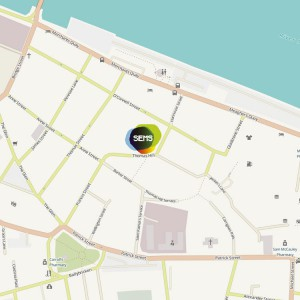
\includegraphics[width=5cm]{images/sems_1}
		%	\caption{ABC}
		\label{fig:logo1}
	\end{figure}
	%
	
	Address: South East Makerspace, Old Printworks, Thomas Hill, Waterford City, Ireland, X91 TW63. (info@southeastmakerspace.org)
\end{frame}


\section{Projects}
\begin{frame}{Projects}
Sample of the projects completed/inprogress by members at SEMS
\begin{itemize}
	\item Billberry Goats
	\item Digistreets (Magical Mushrooms, Trash Talk)
	\item Floppy Drive Midi Player
	\item 3D Printer
	\item Quadcopter Drone
	\item 4x4x4 LED Cube
	\item Red Phone
	\item Bartop Game Arcade
	\item Jigsaw Dinosaurs
\end{itemize}
\end{frame}

\section{Bilberry Goats Exhibition}
\begin{frame}{Bilberry Goats Exhibition}
	\begin{figure}
		\begin{tabular}{ccc}
			\subfloat{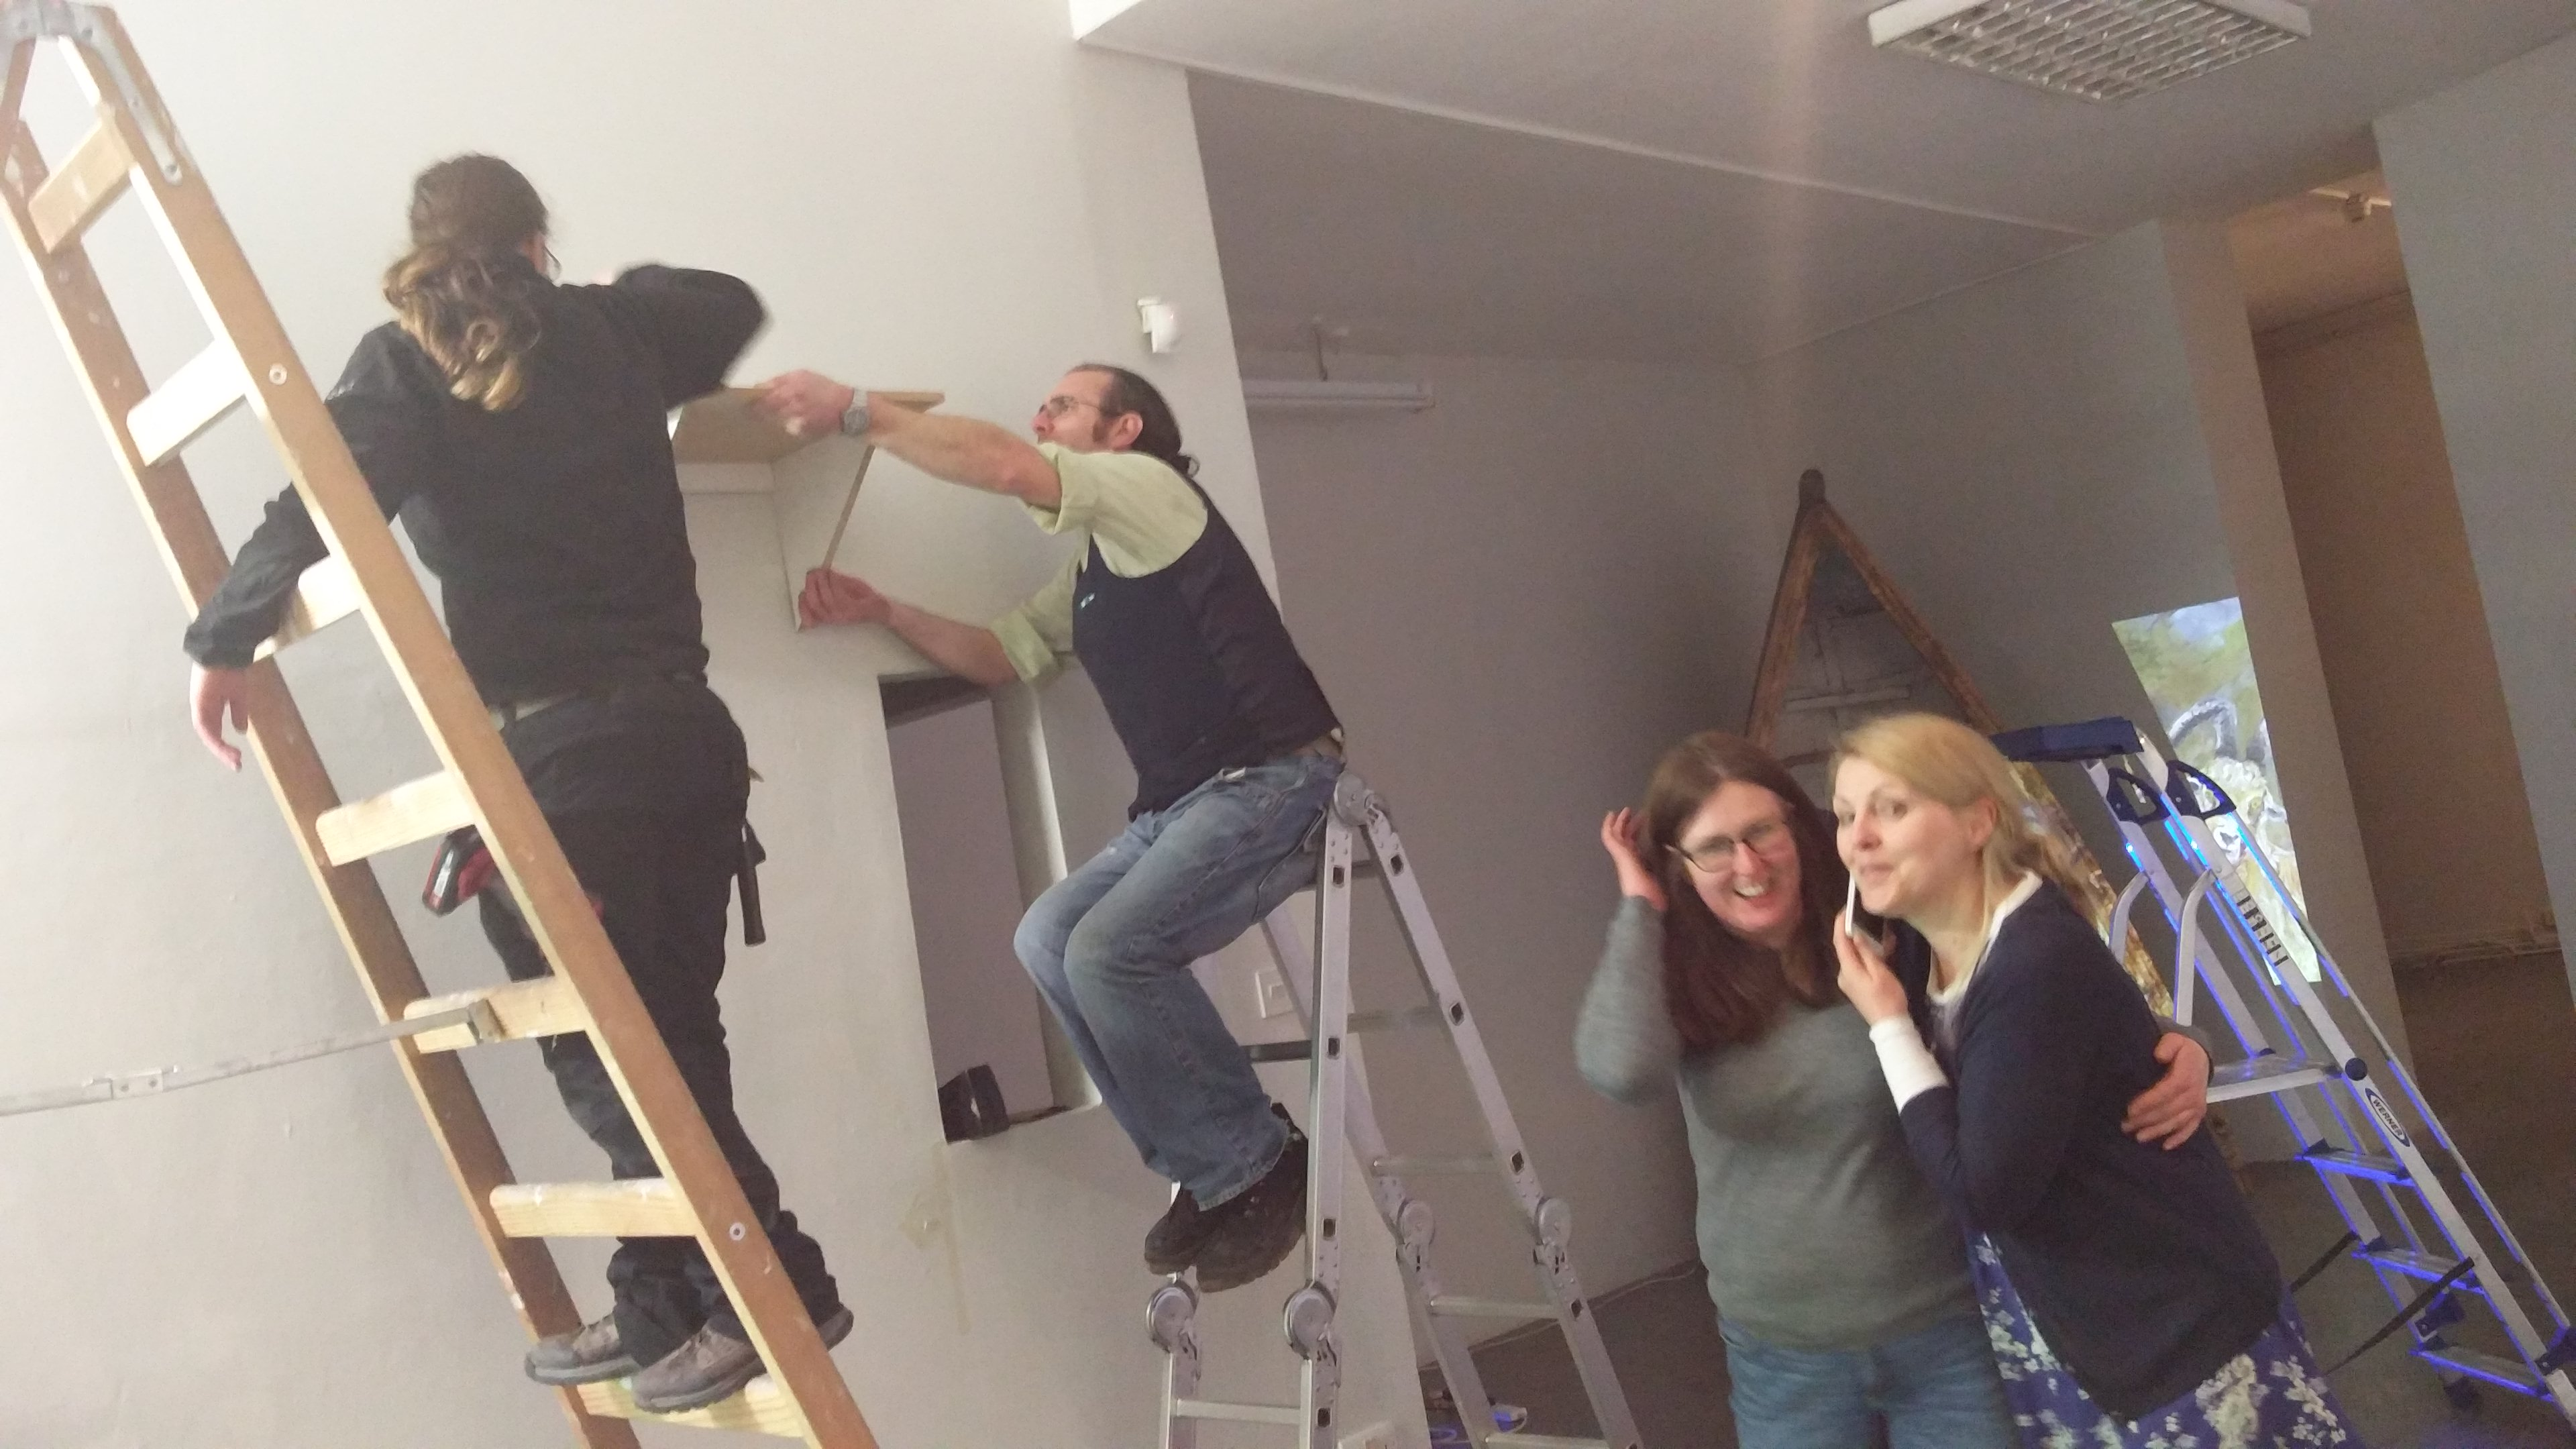
\includegraphics[width = 1.3in]{images/bilberry_1}} &
			\subfloat{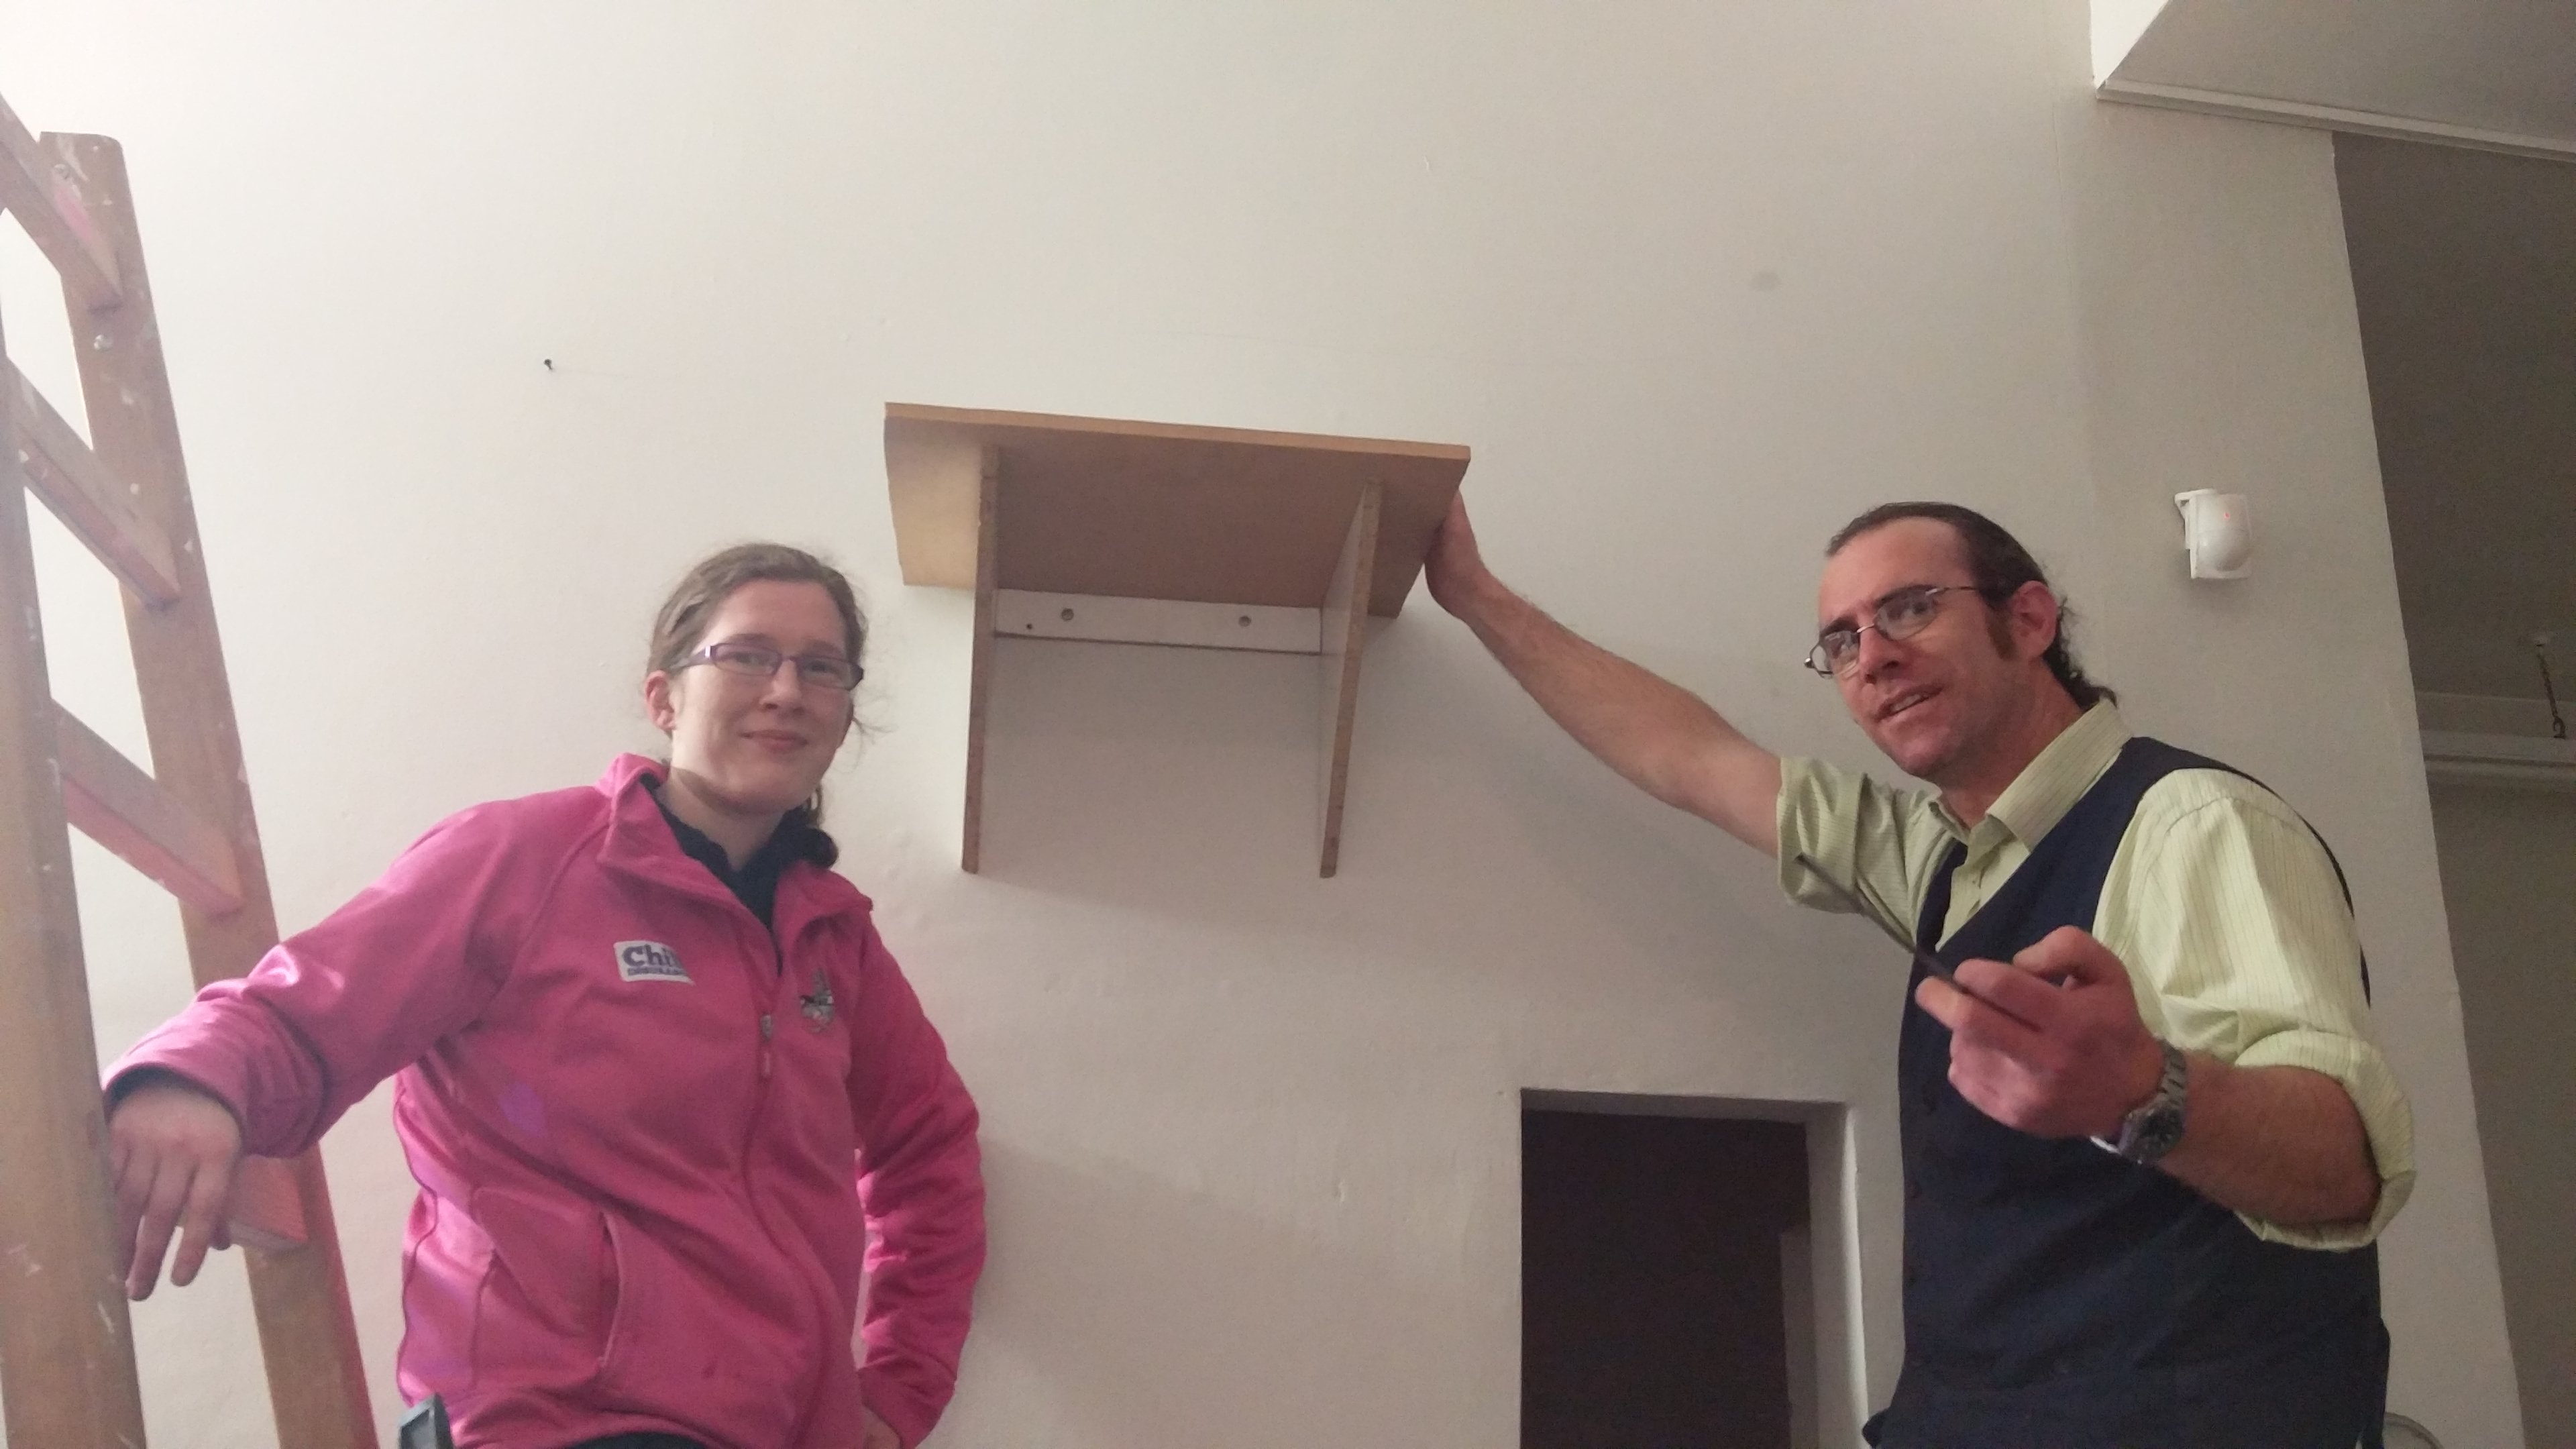
\includegraphics[width = 1.3in]{images/bilberry_2}} &
			\subfloat{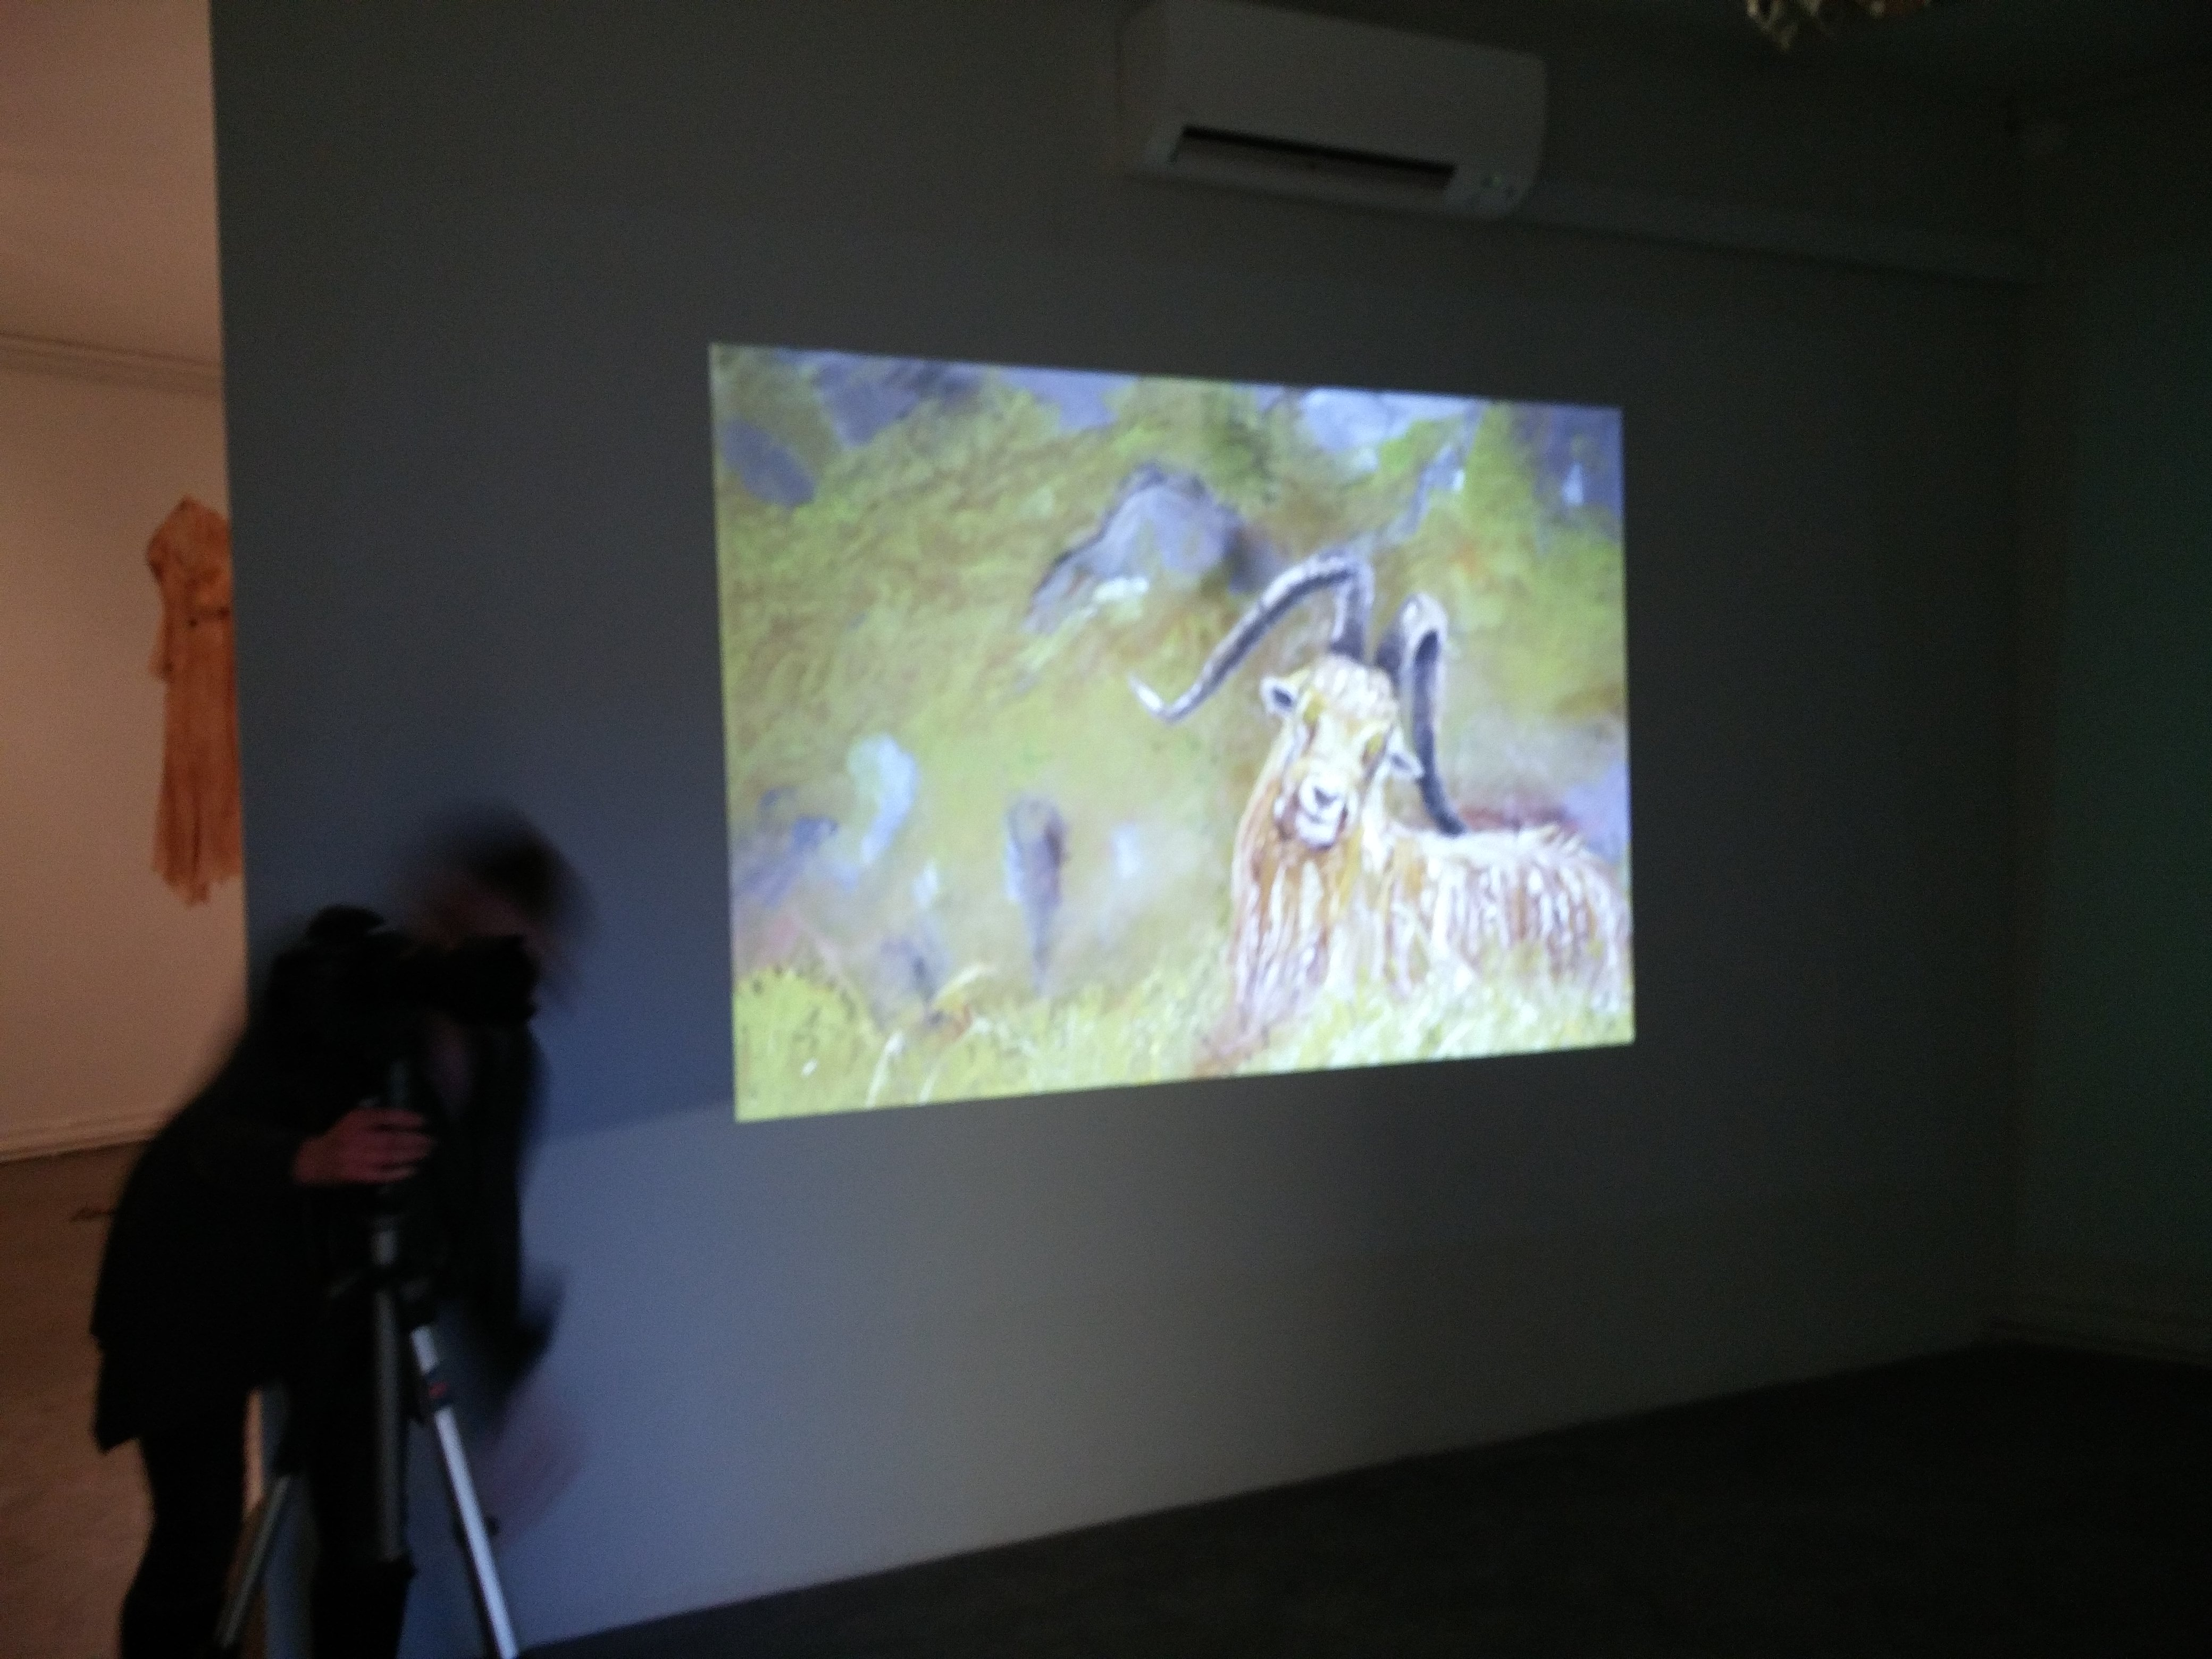
\includegraphics[width = 1.3in]{images/bilberry_3}} \\
			\subfloat{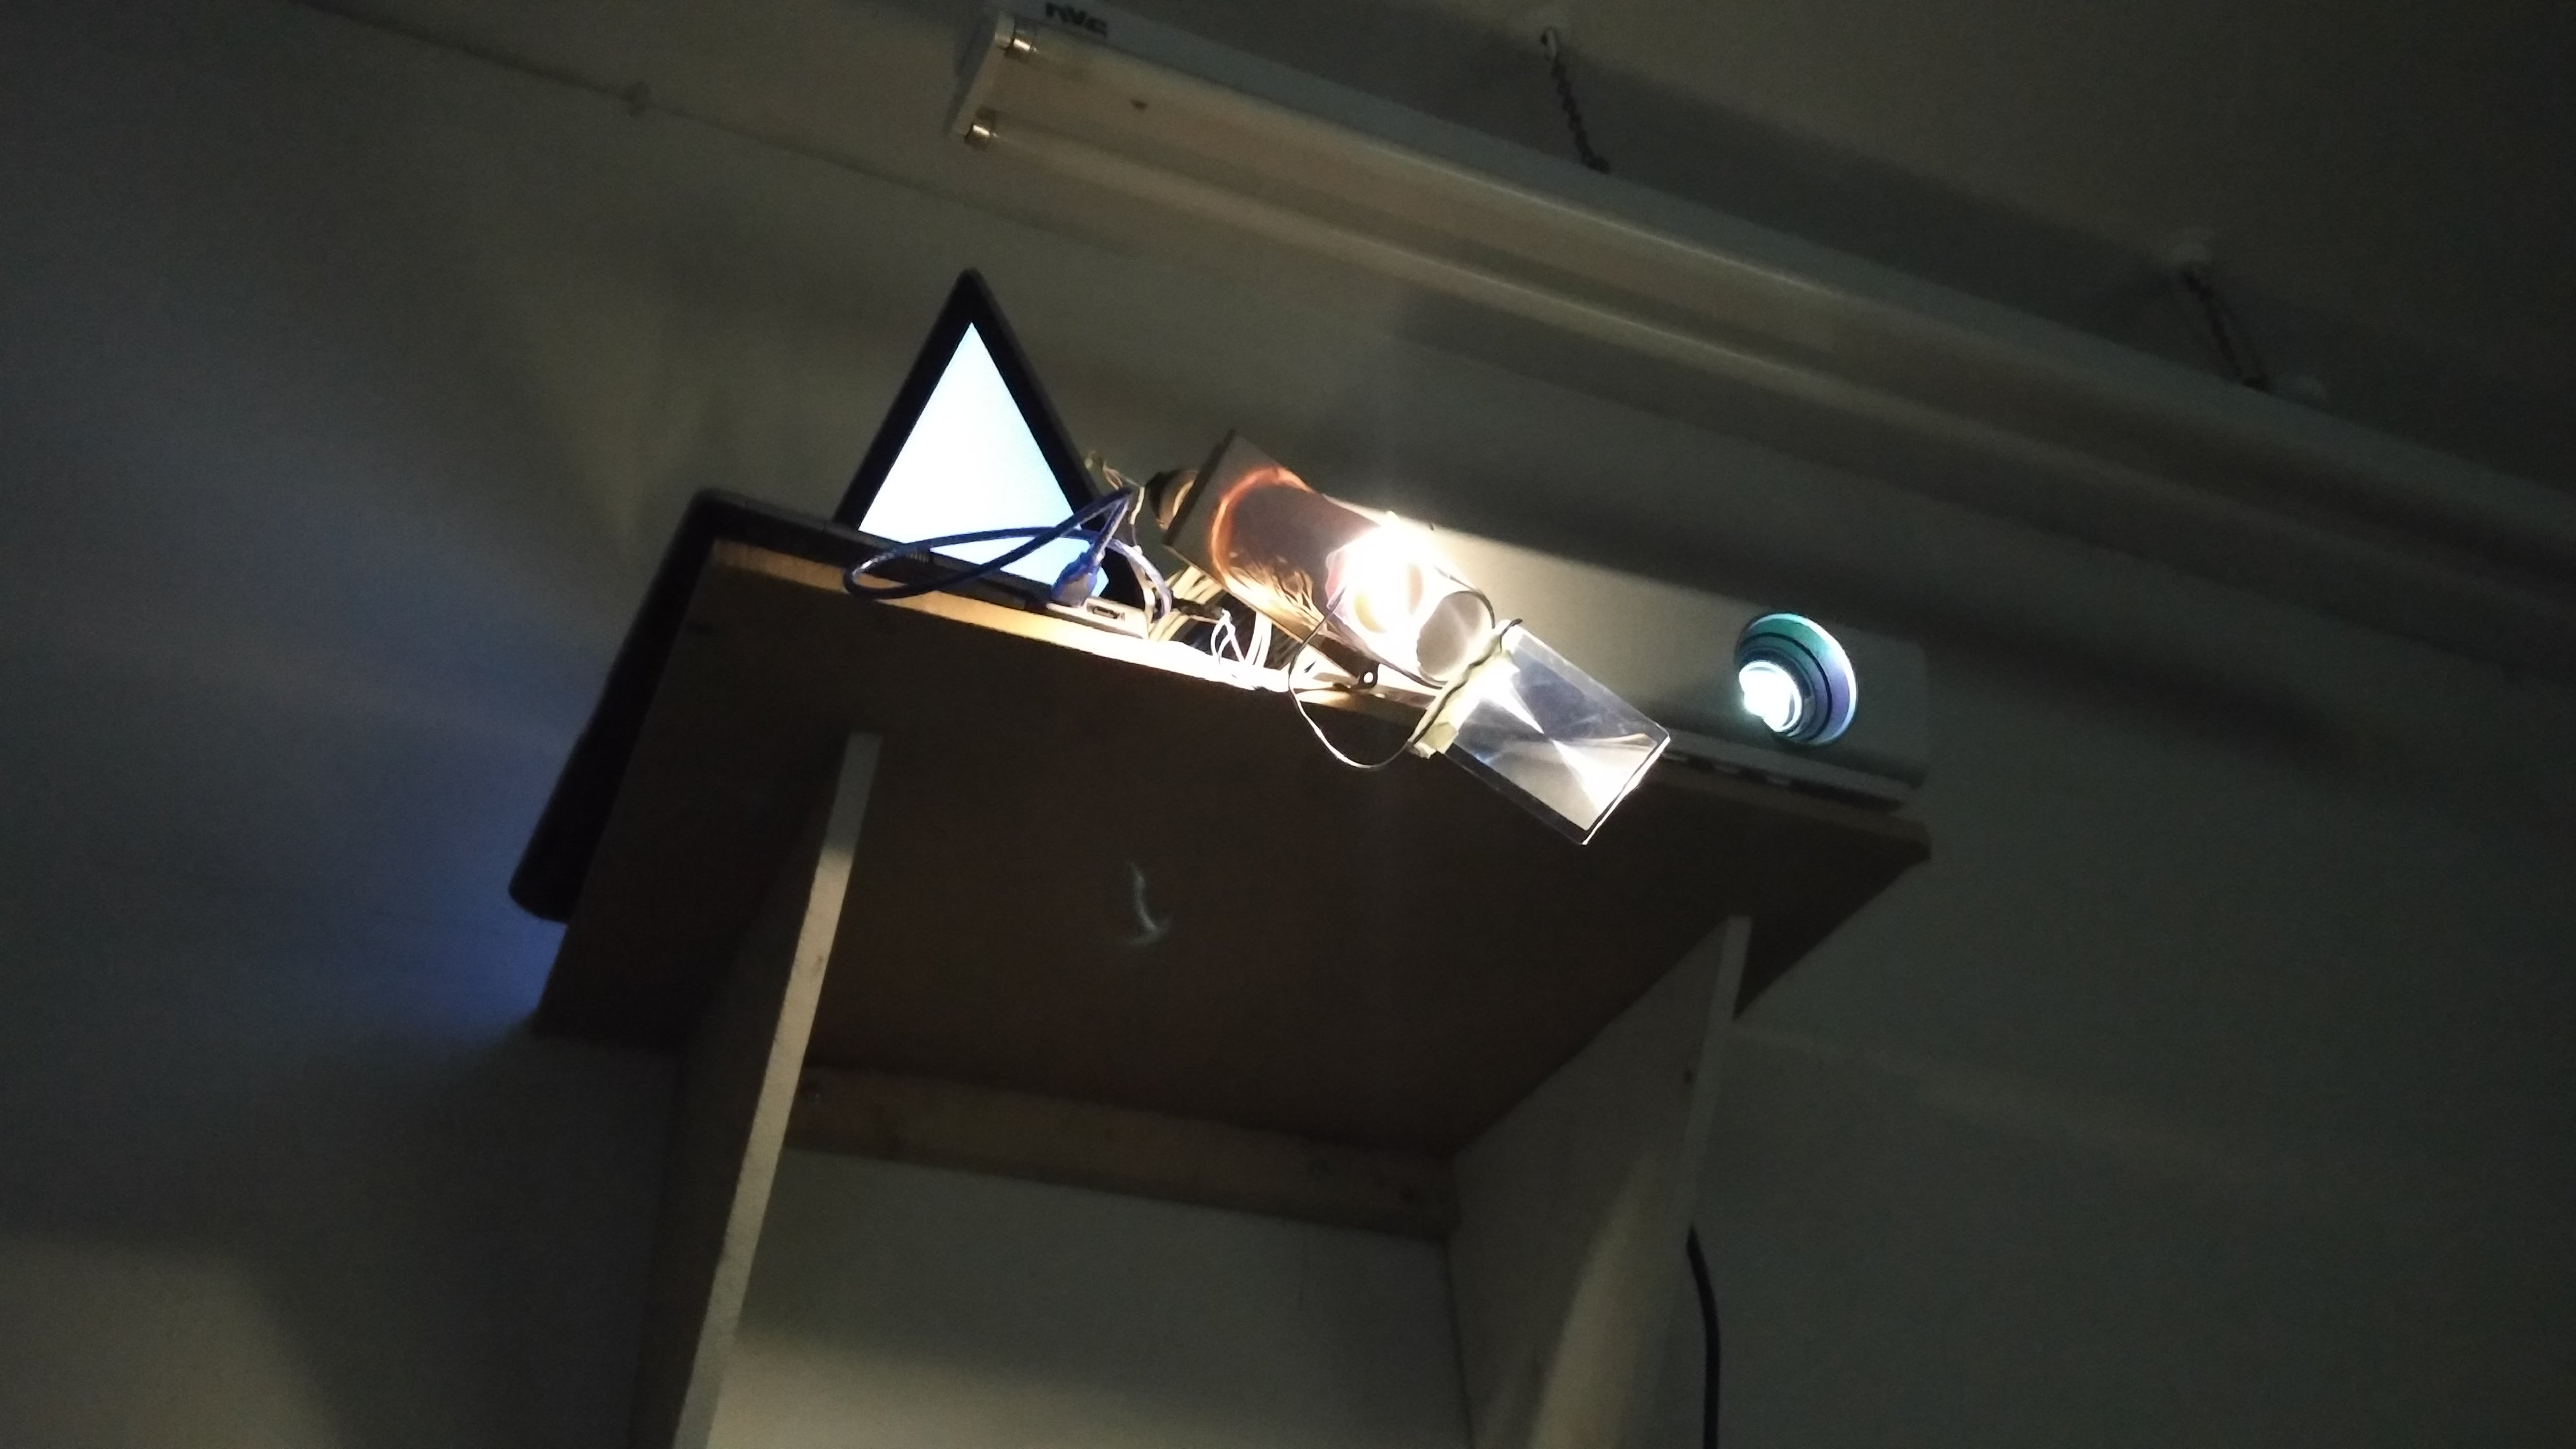
\includegraphics[width = 1.3in]{images/bilberry_4}} &    \subfloat{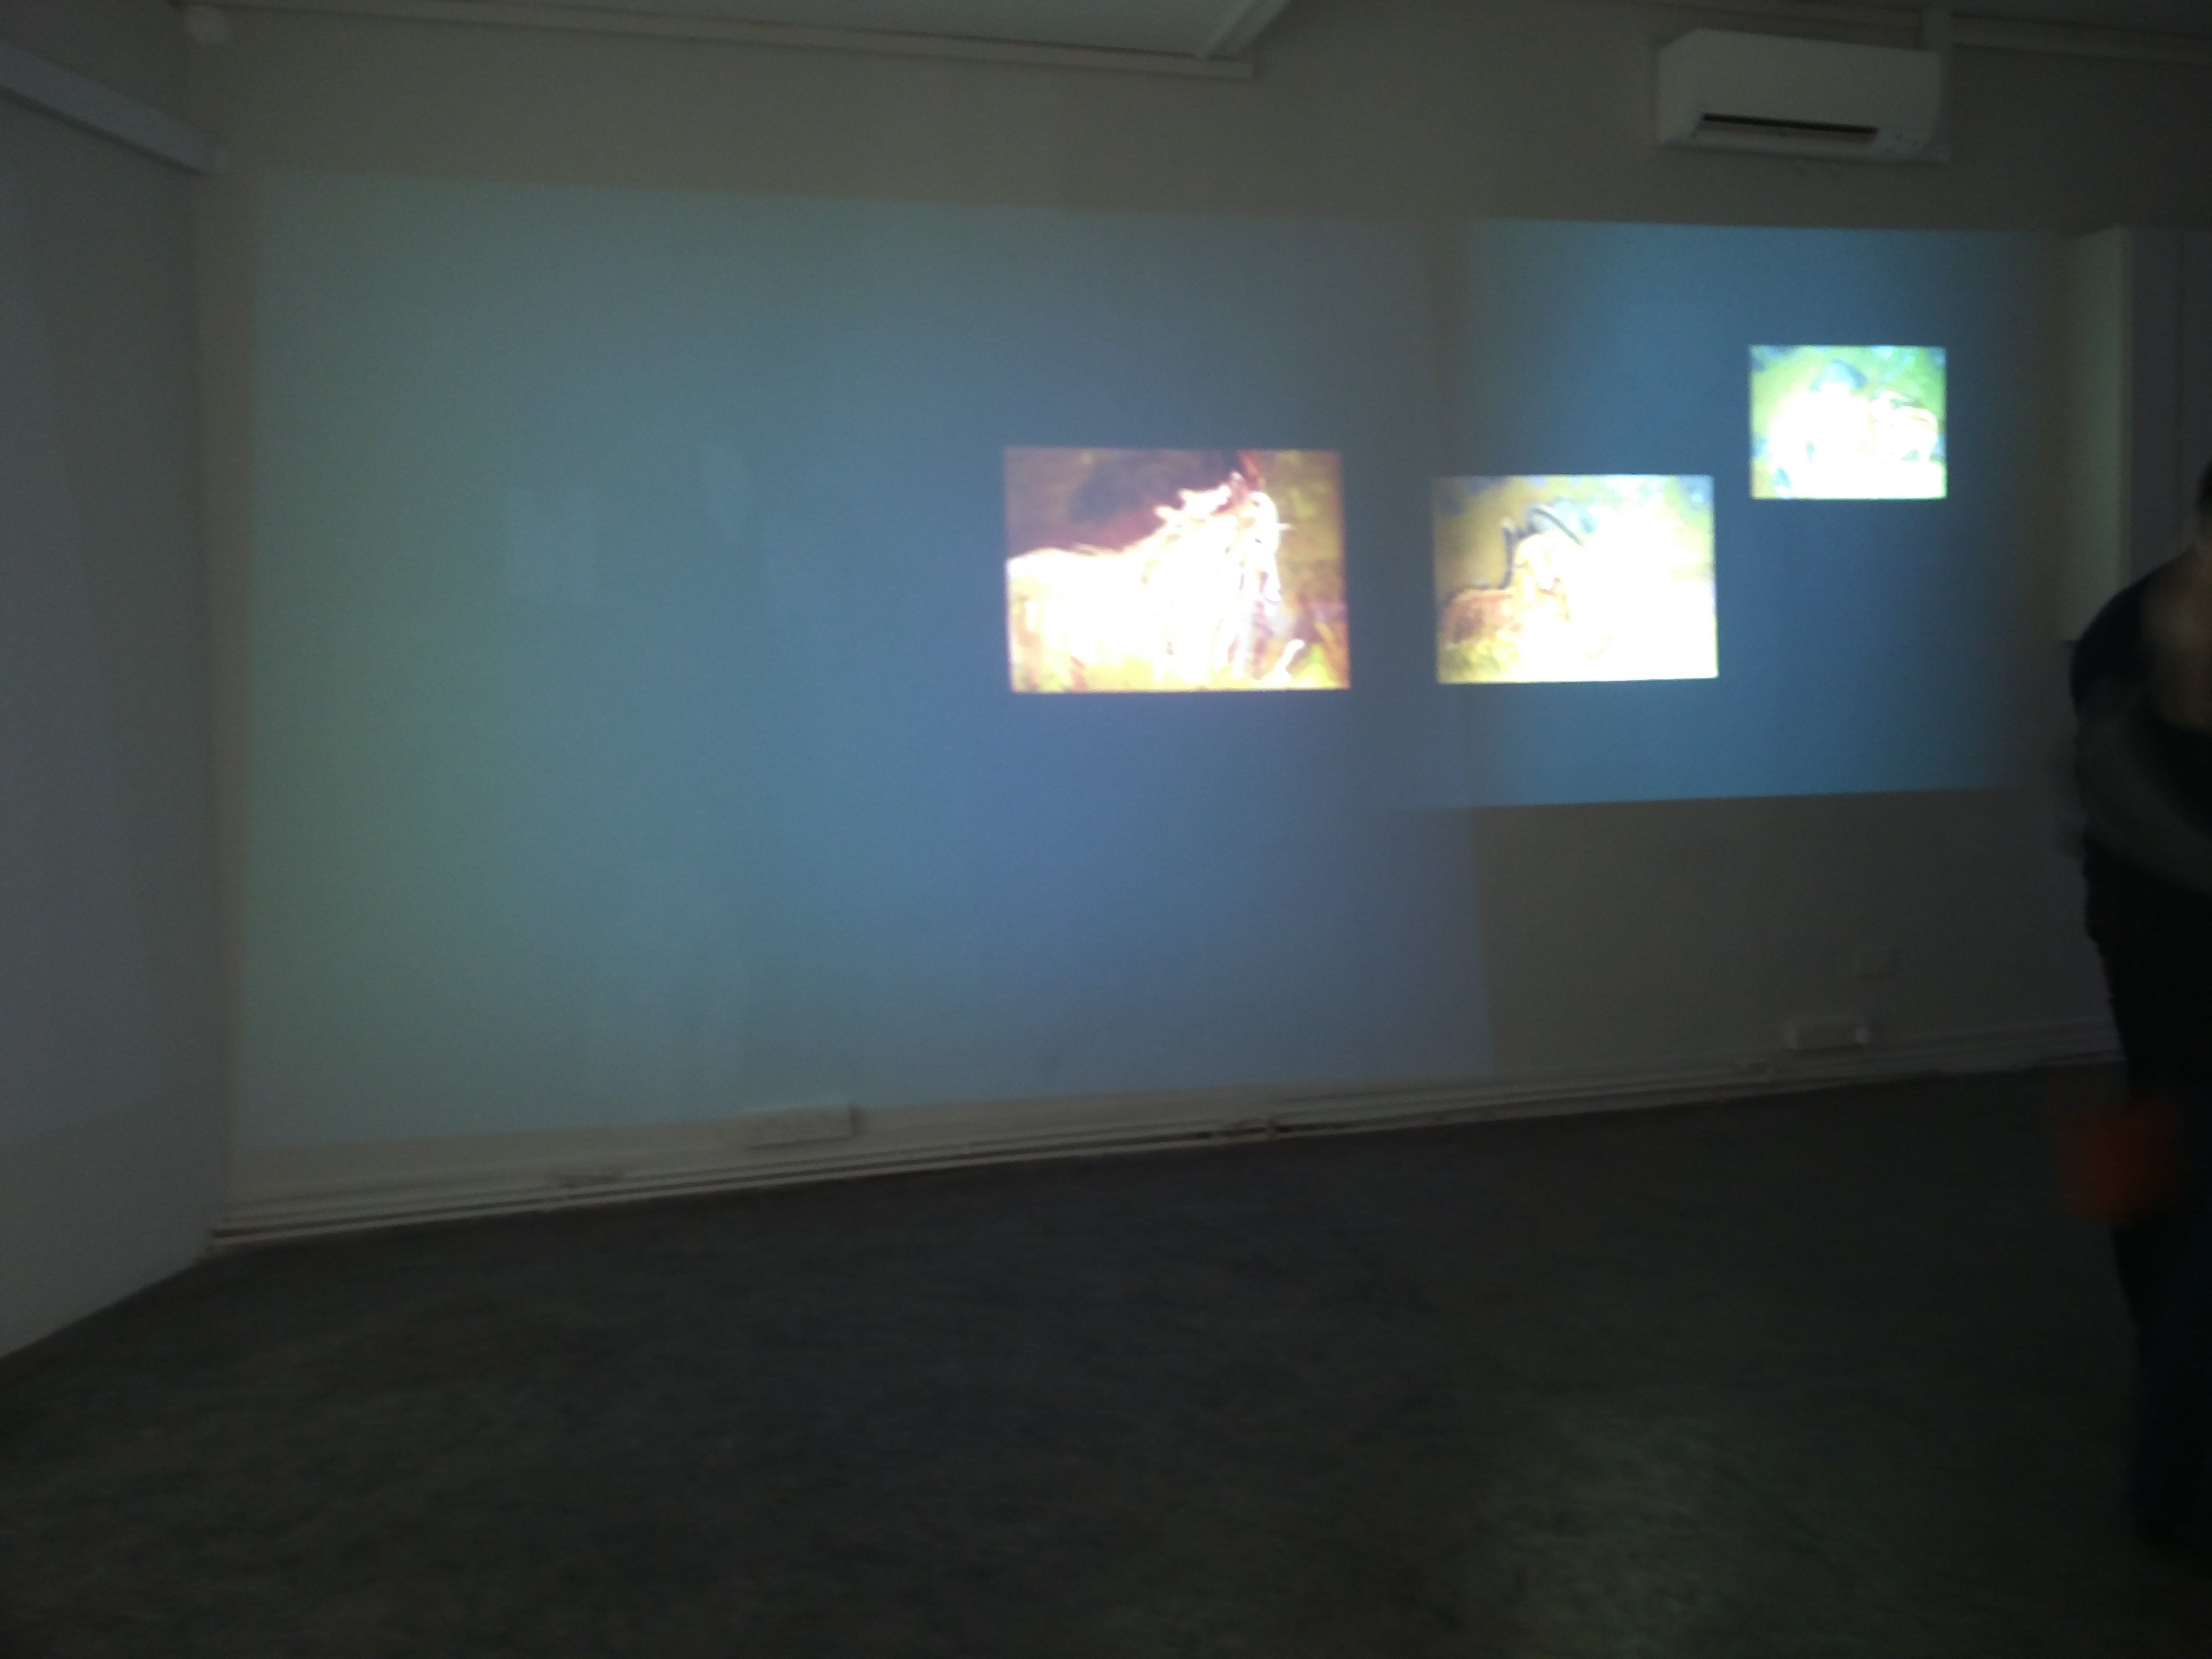
\includegraphics[width = 1.3in]{images/bilberry_5}} &
			\subfloat{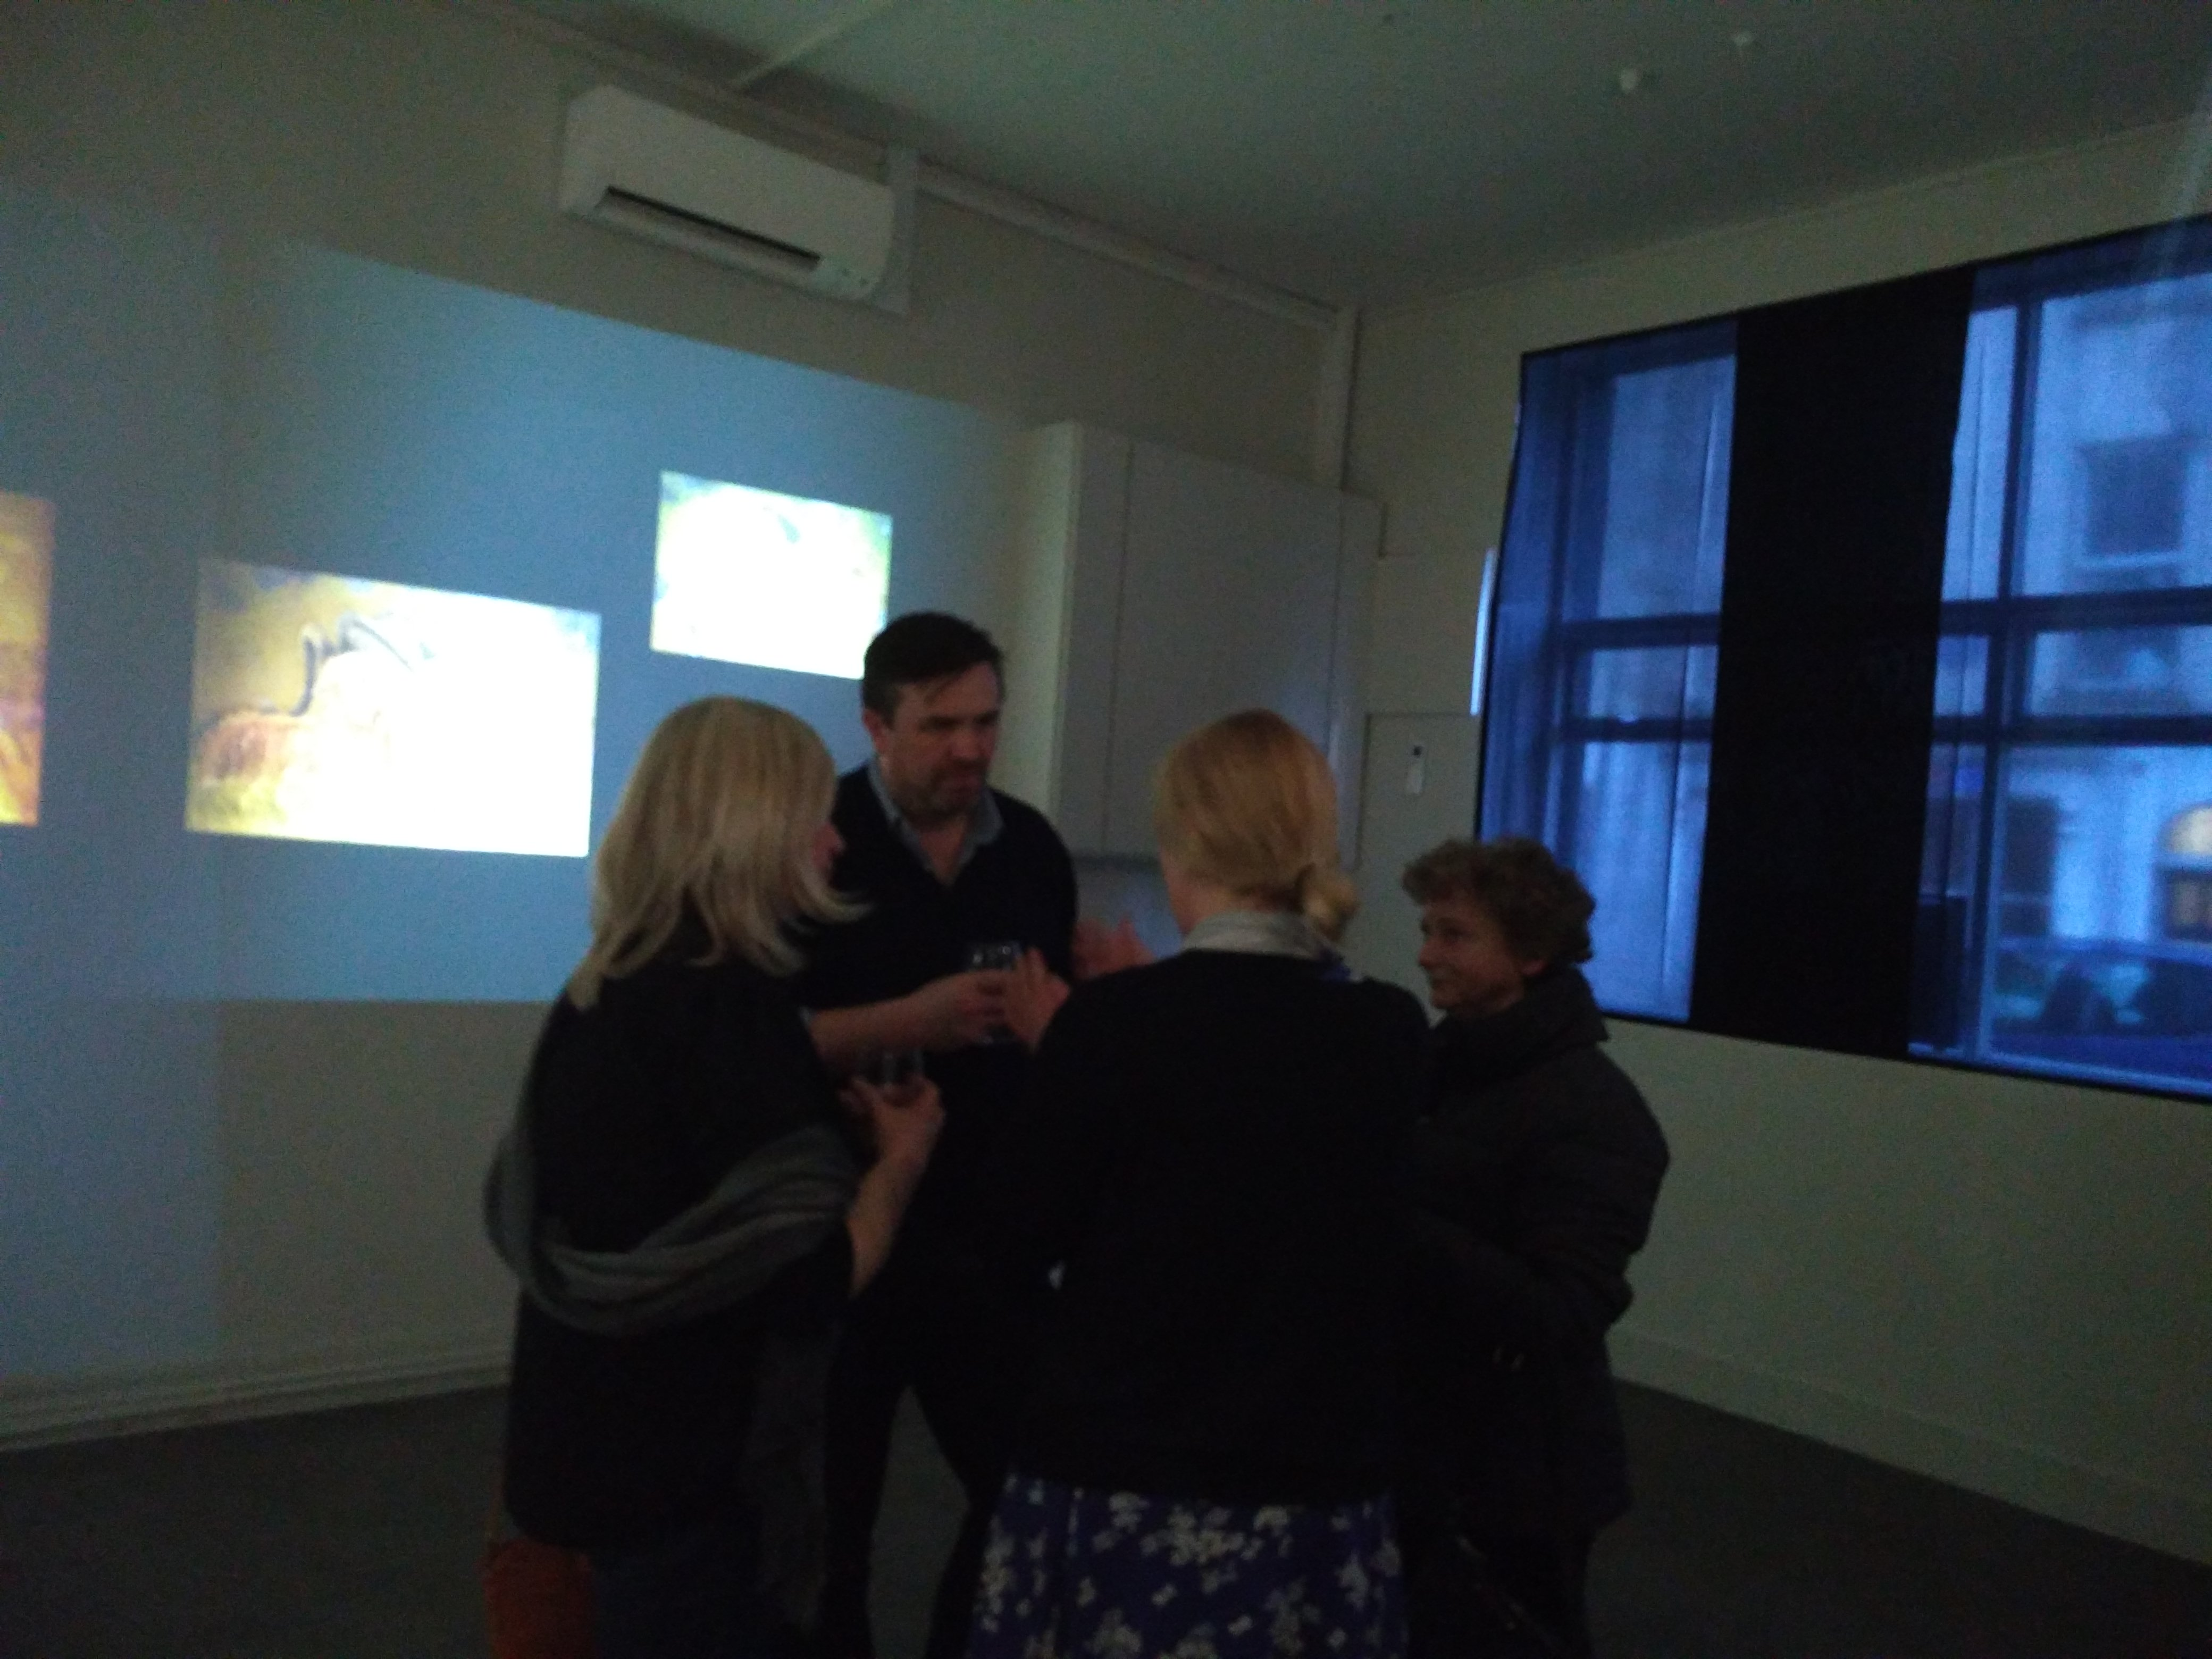
\includegraphics[width = 1.3in]{images/bilberry_6}} 
		\end{tabular}
		\caption{Bilberry Goat Art Exhibition at GOMA Gallery 2017}
	\end{figure}
\end{frame}

\section{Digistreets}
\begin{frame}{Digistreets}
	\begin{figure}
		\begin{tabular}{ccc}
			\subfloat{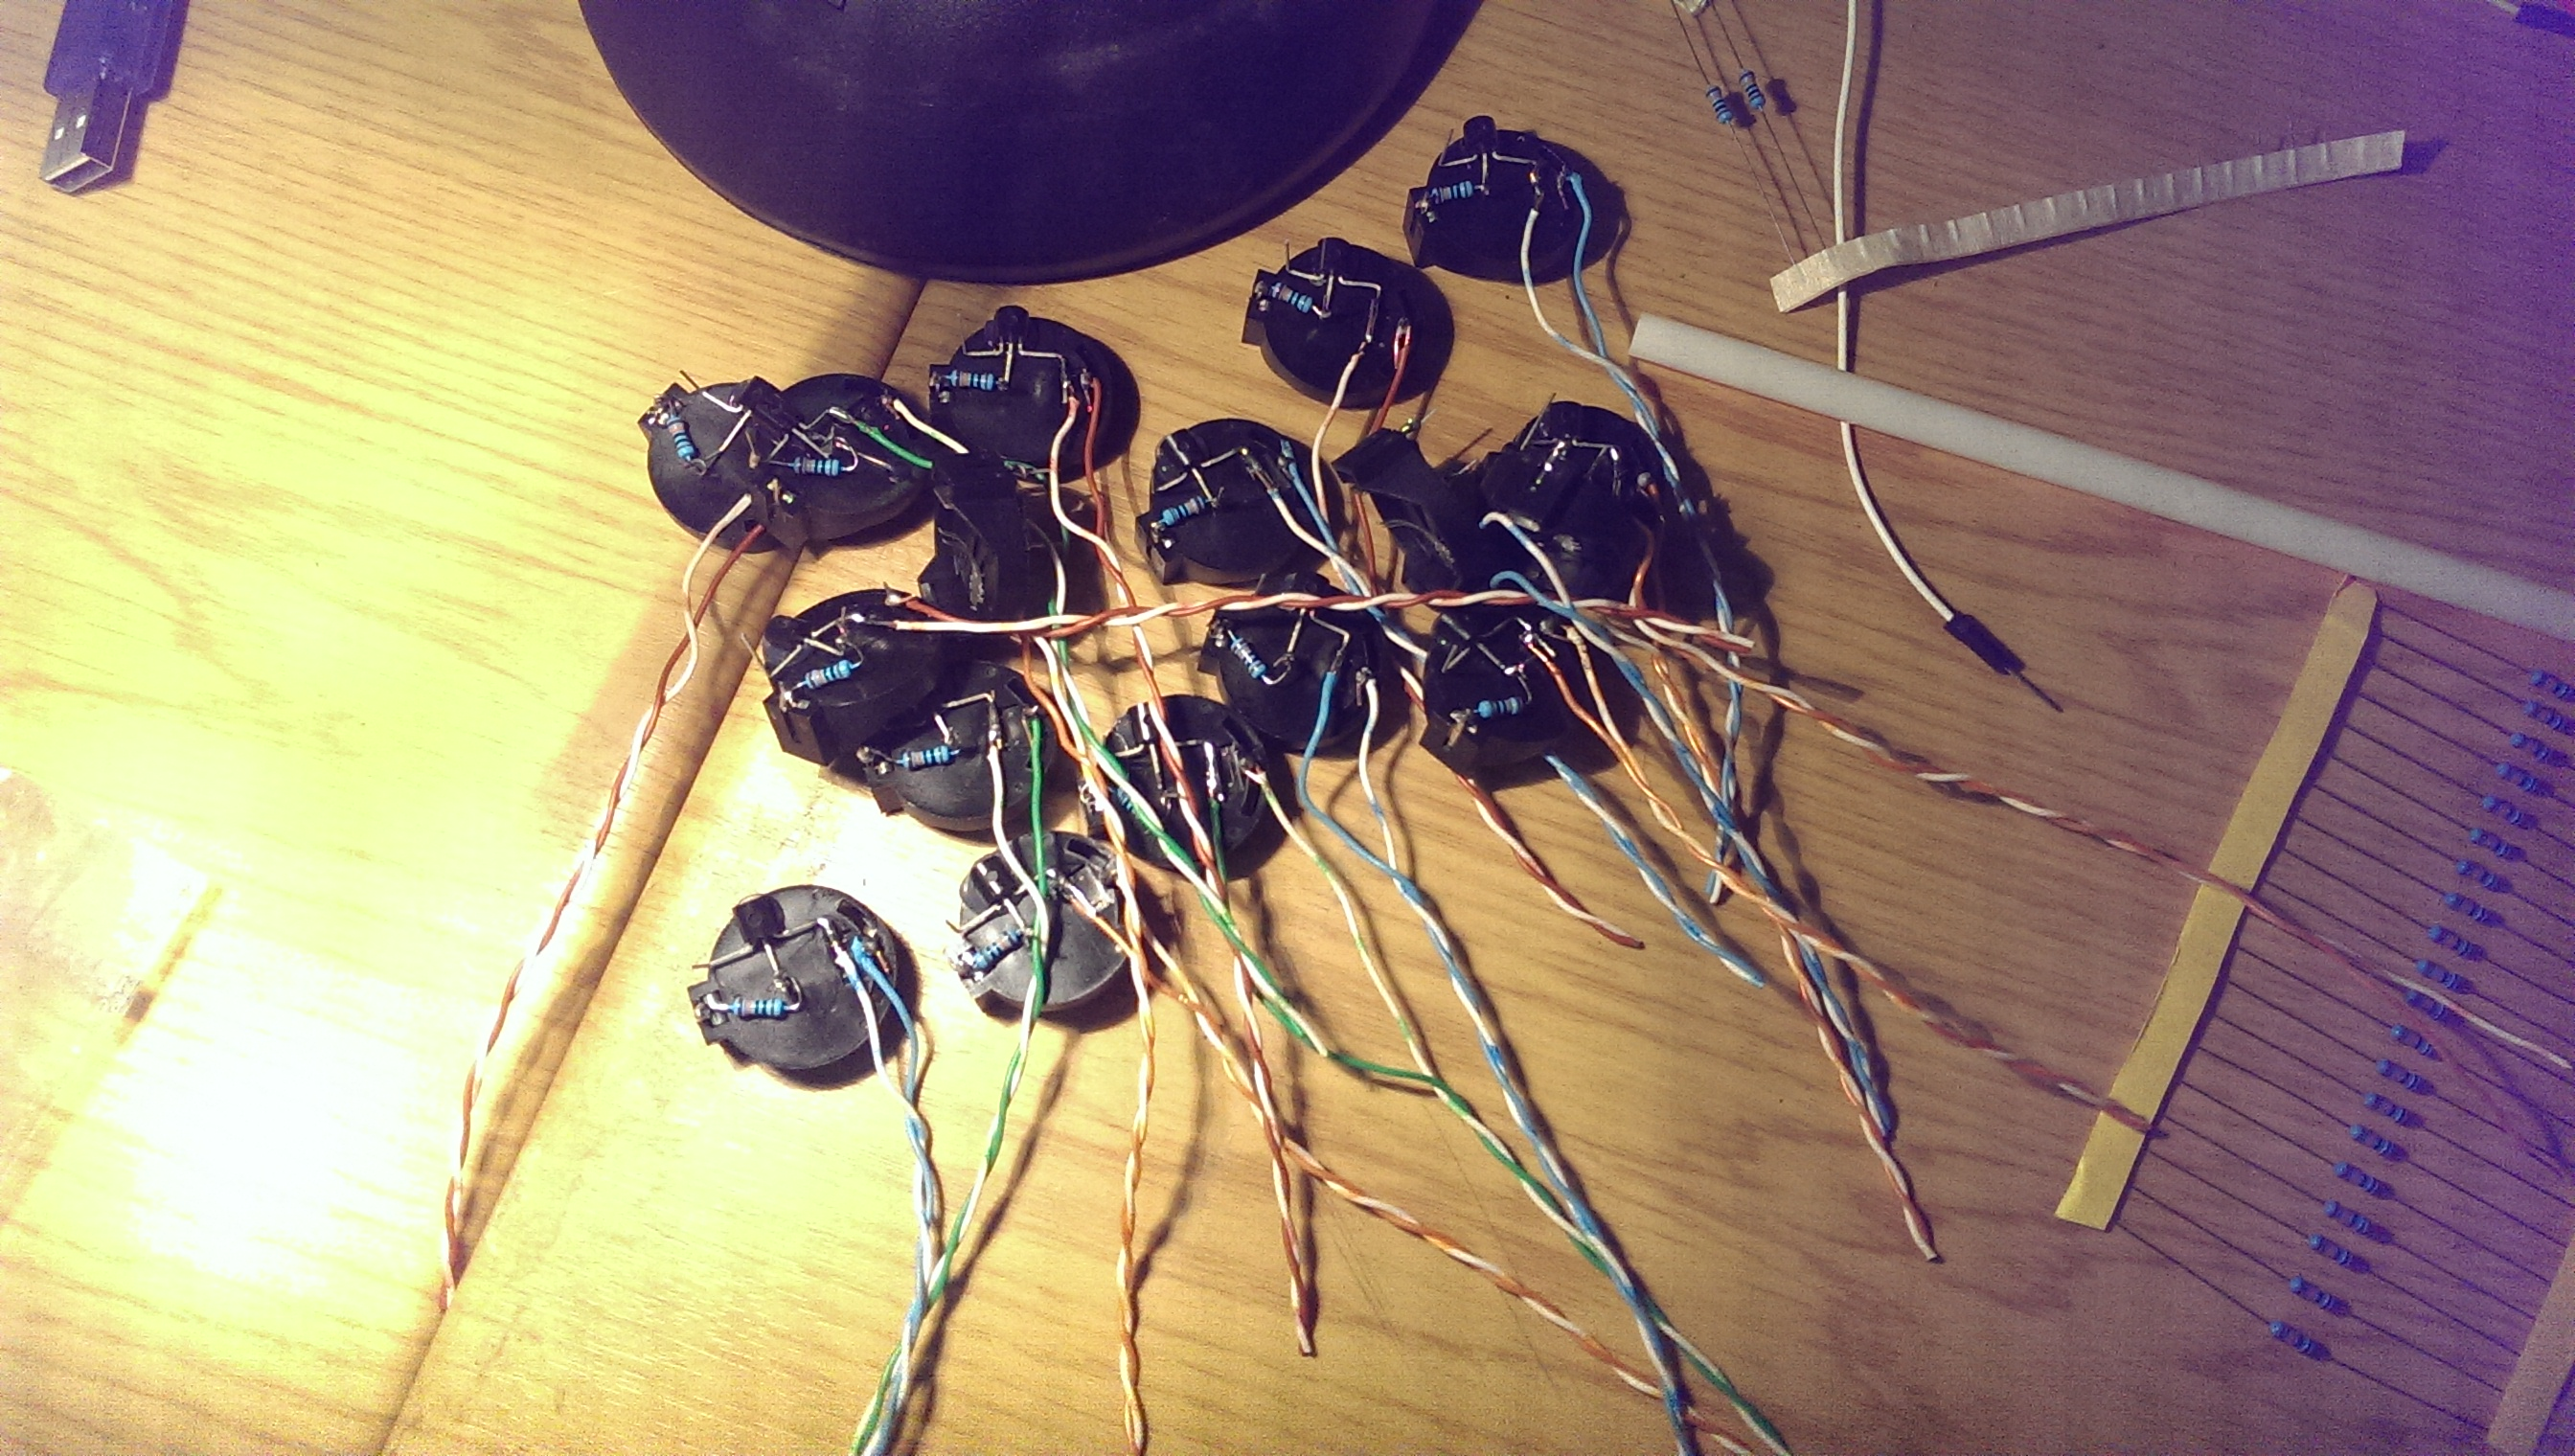
\includegraphics[width = 1.3in]{images/mushrooms_1}} &
			\subfloat[Magic Mushrooms]{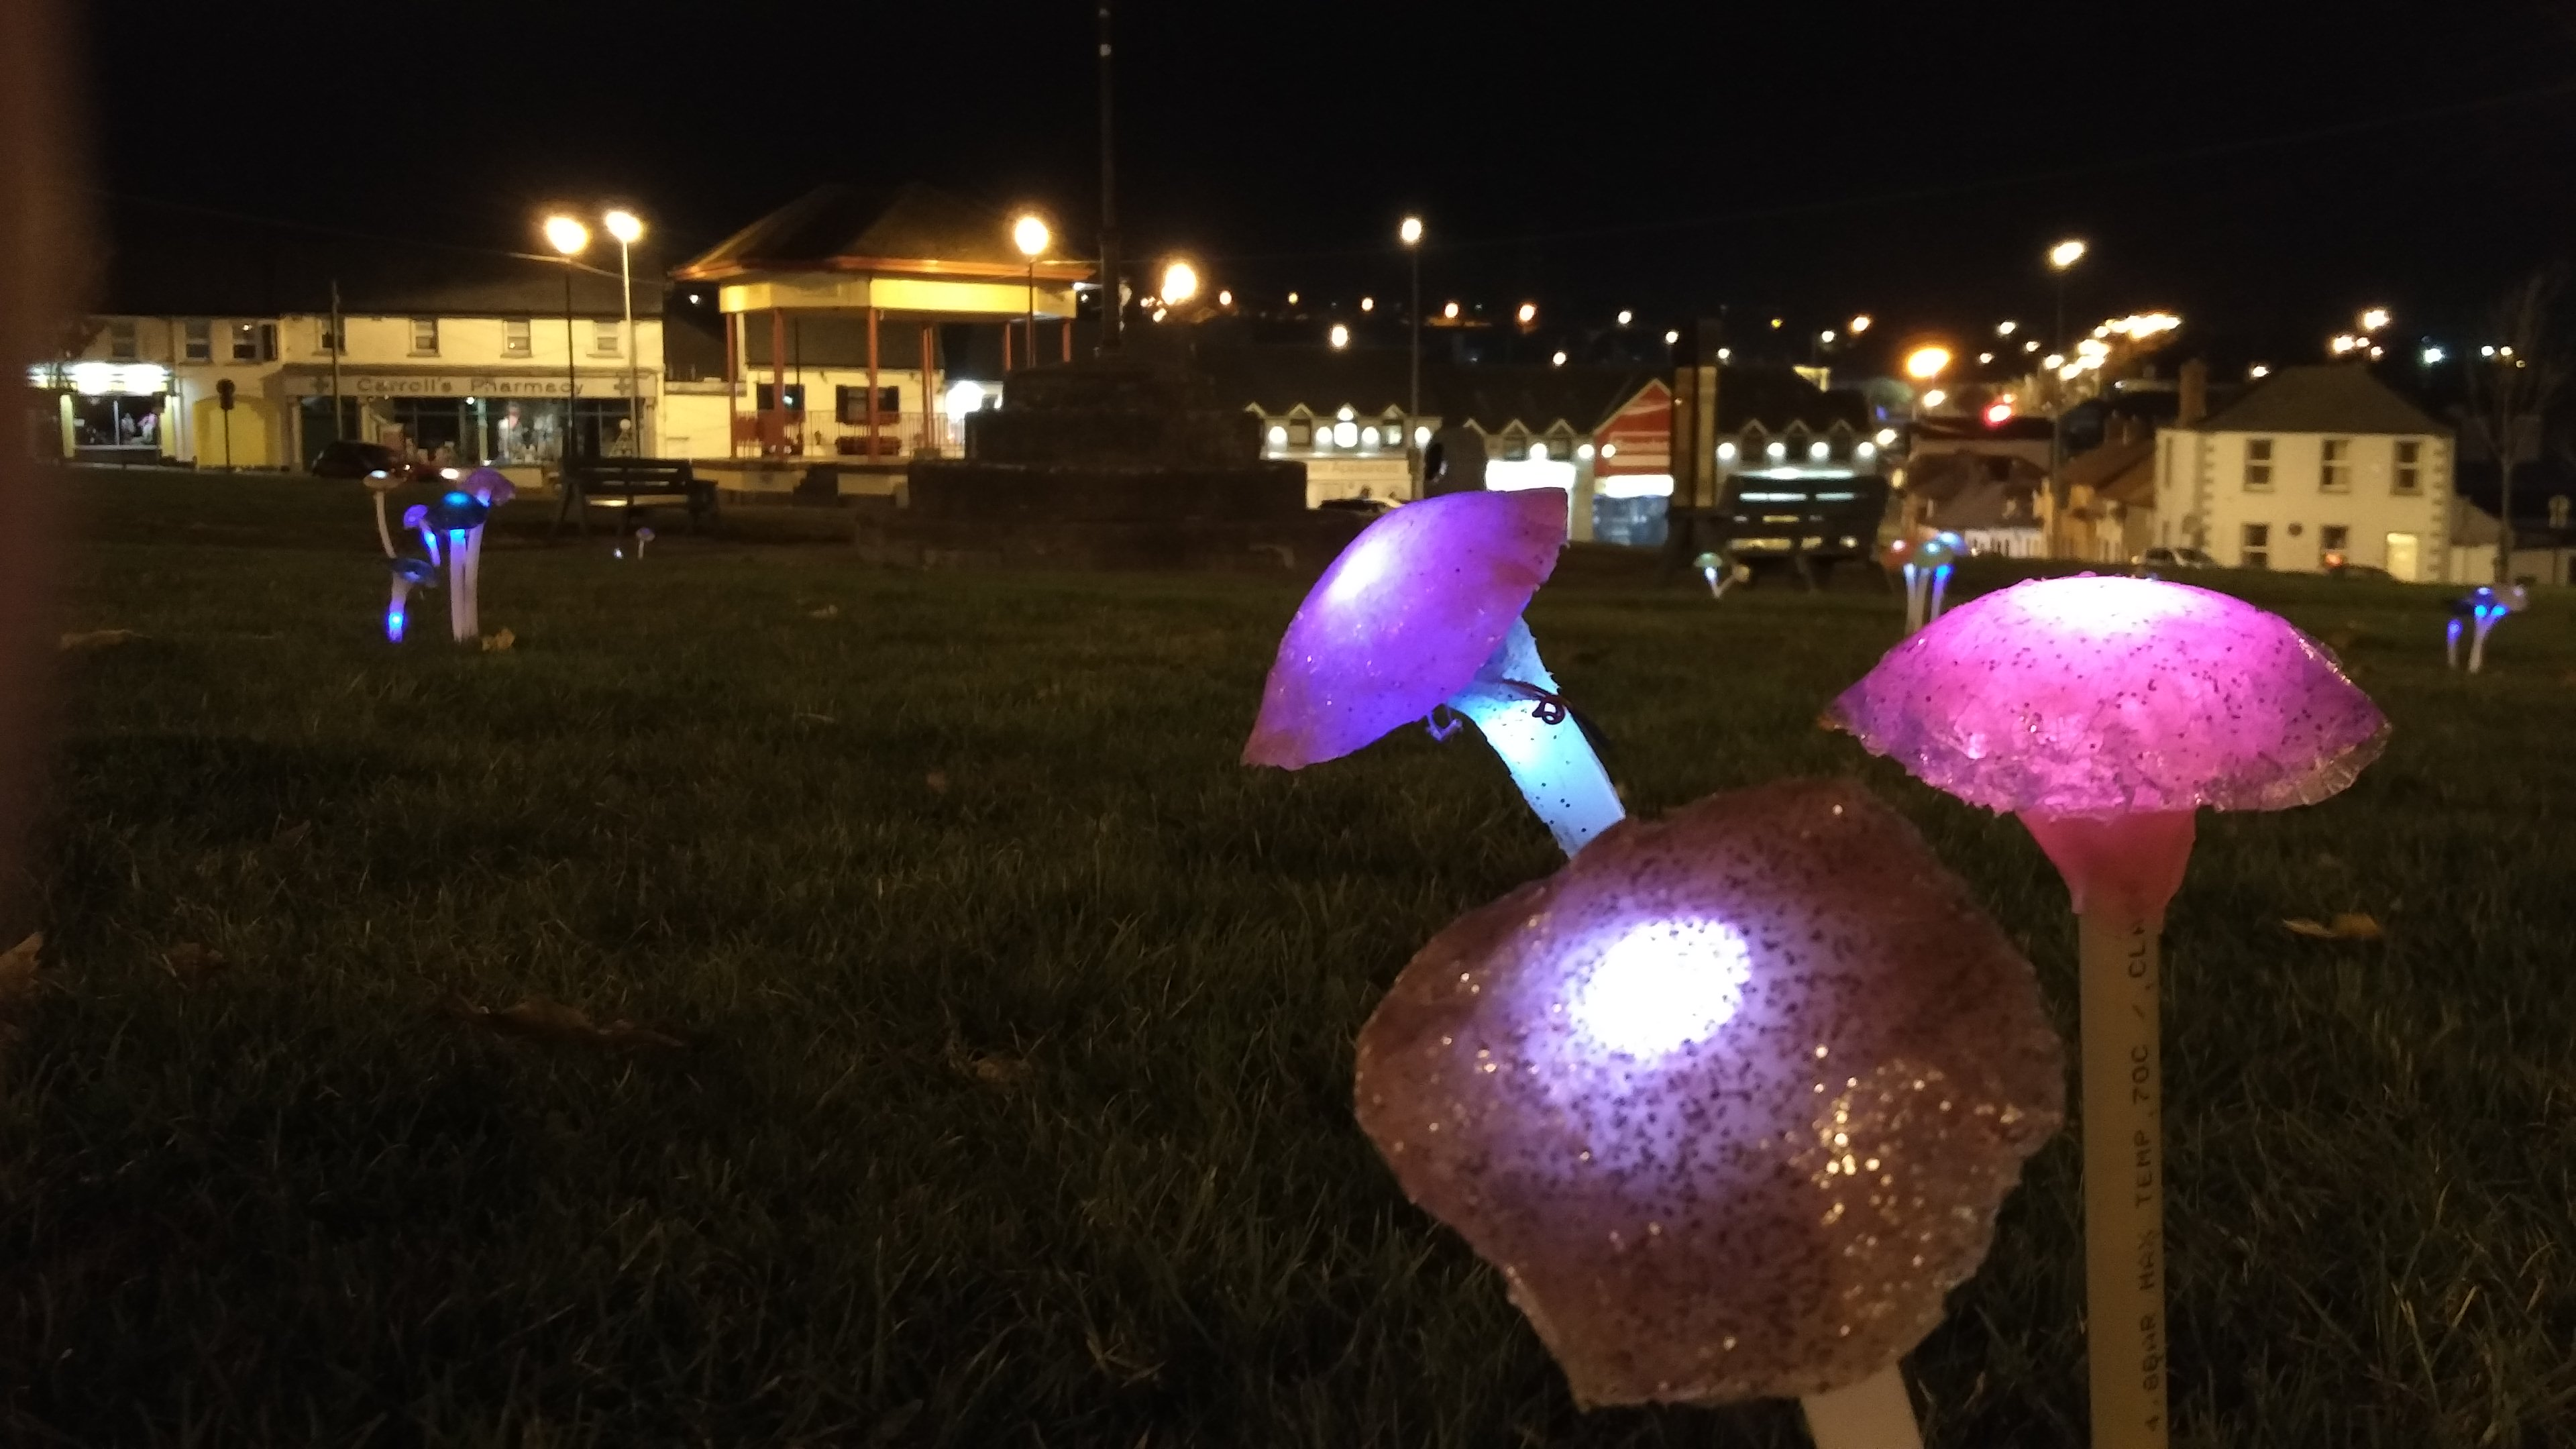
\includegraphics[width = 1.3in]{images/mushrooms_2}} &
			\subfloat{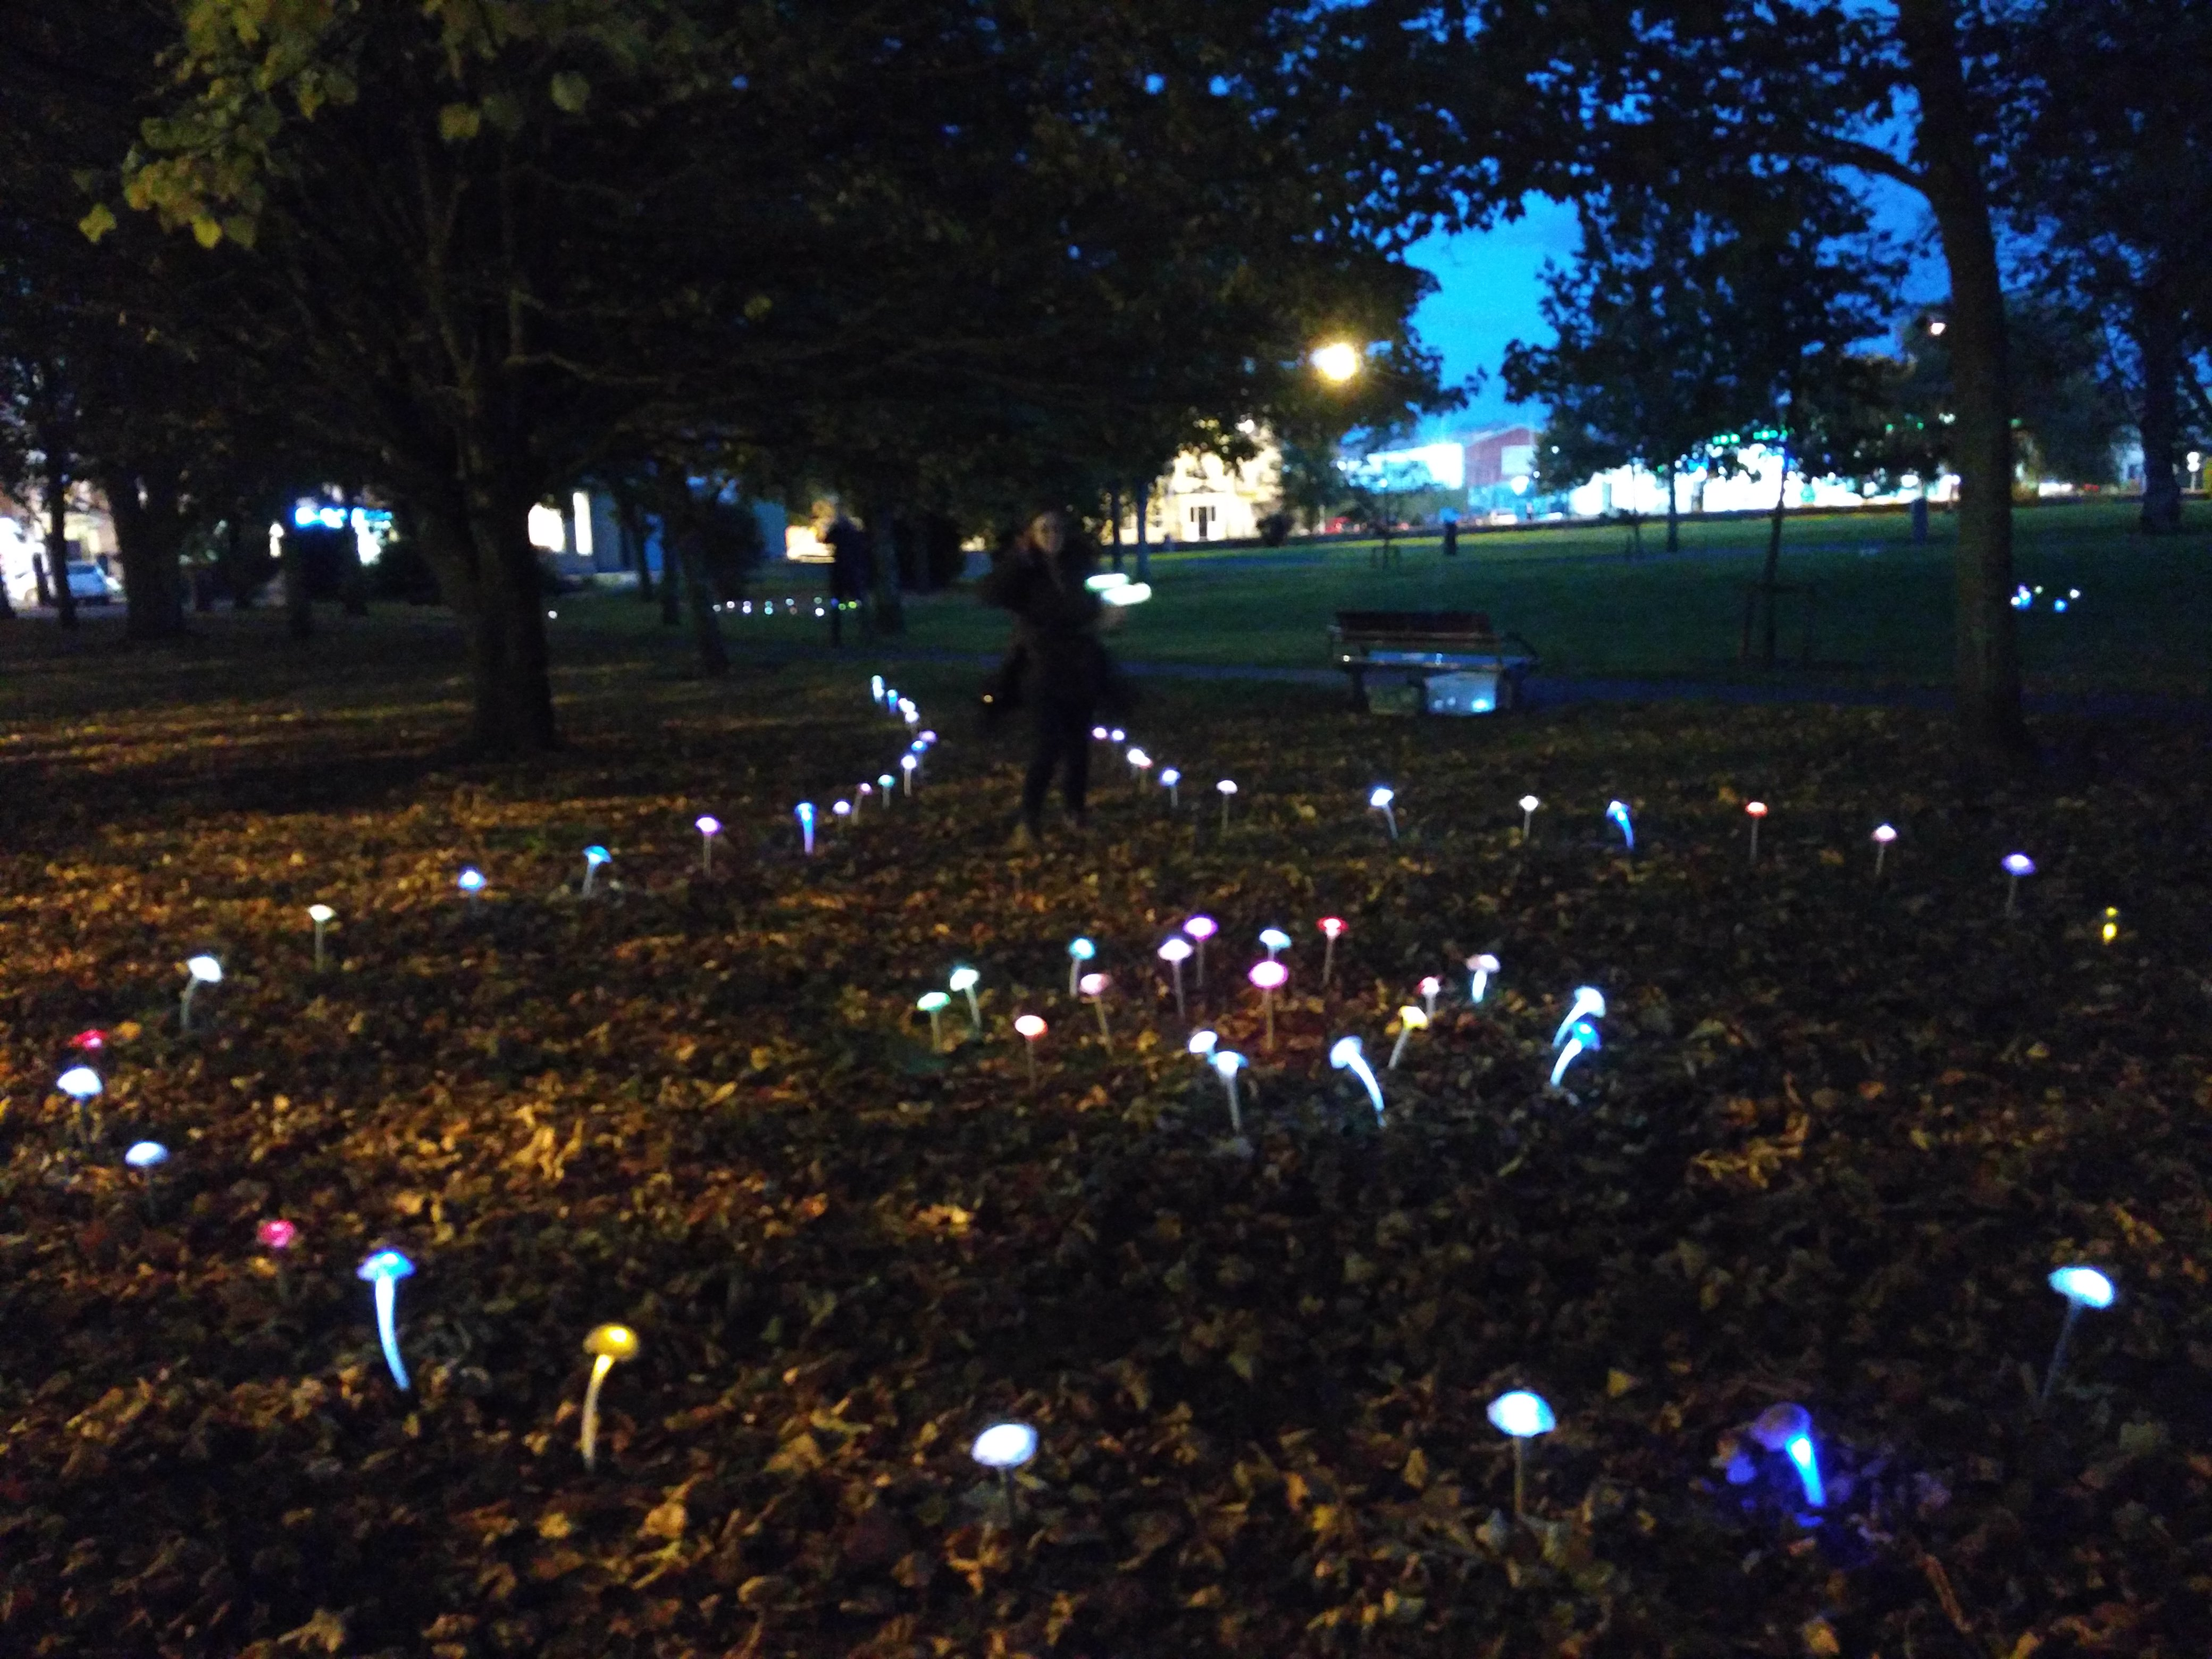
\includegraphics[width = 1.3in]{images/mushrooms_3}} \\
			\subfloat{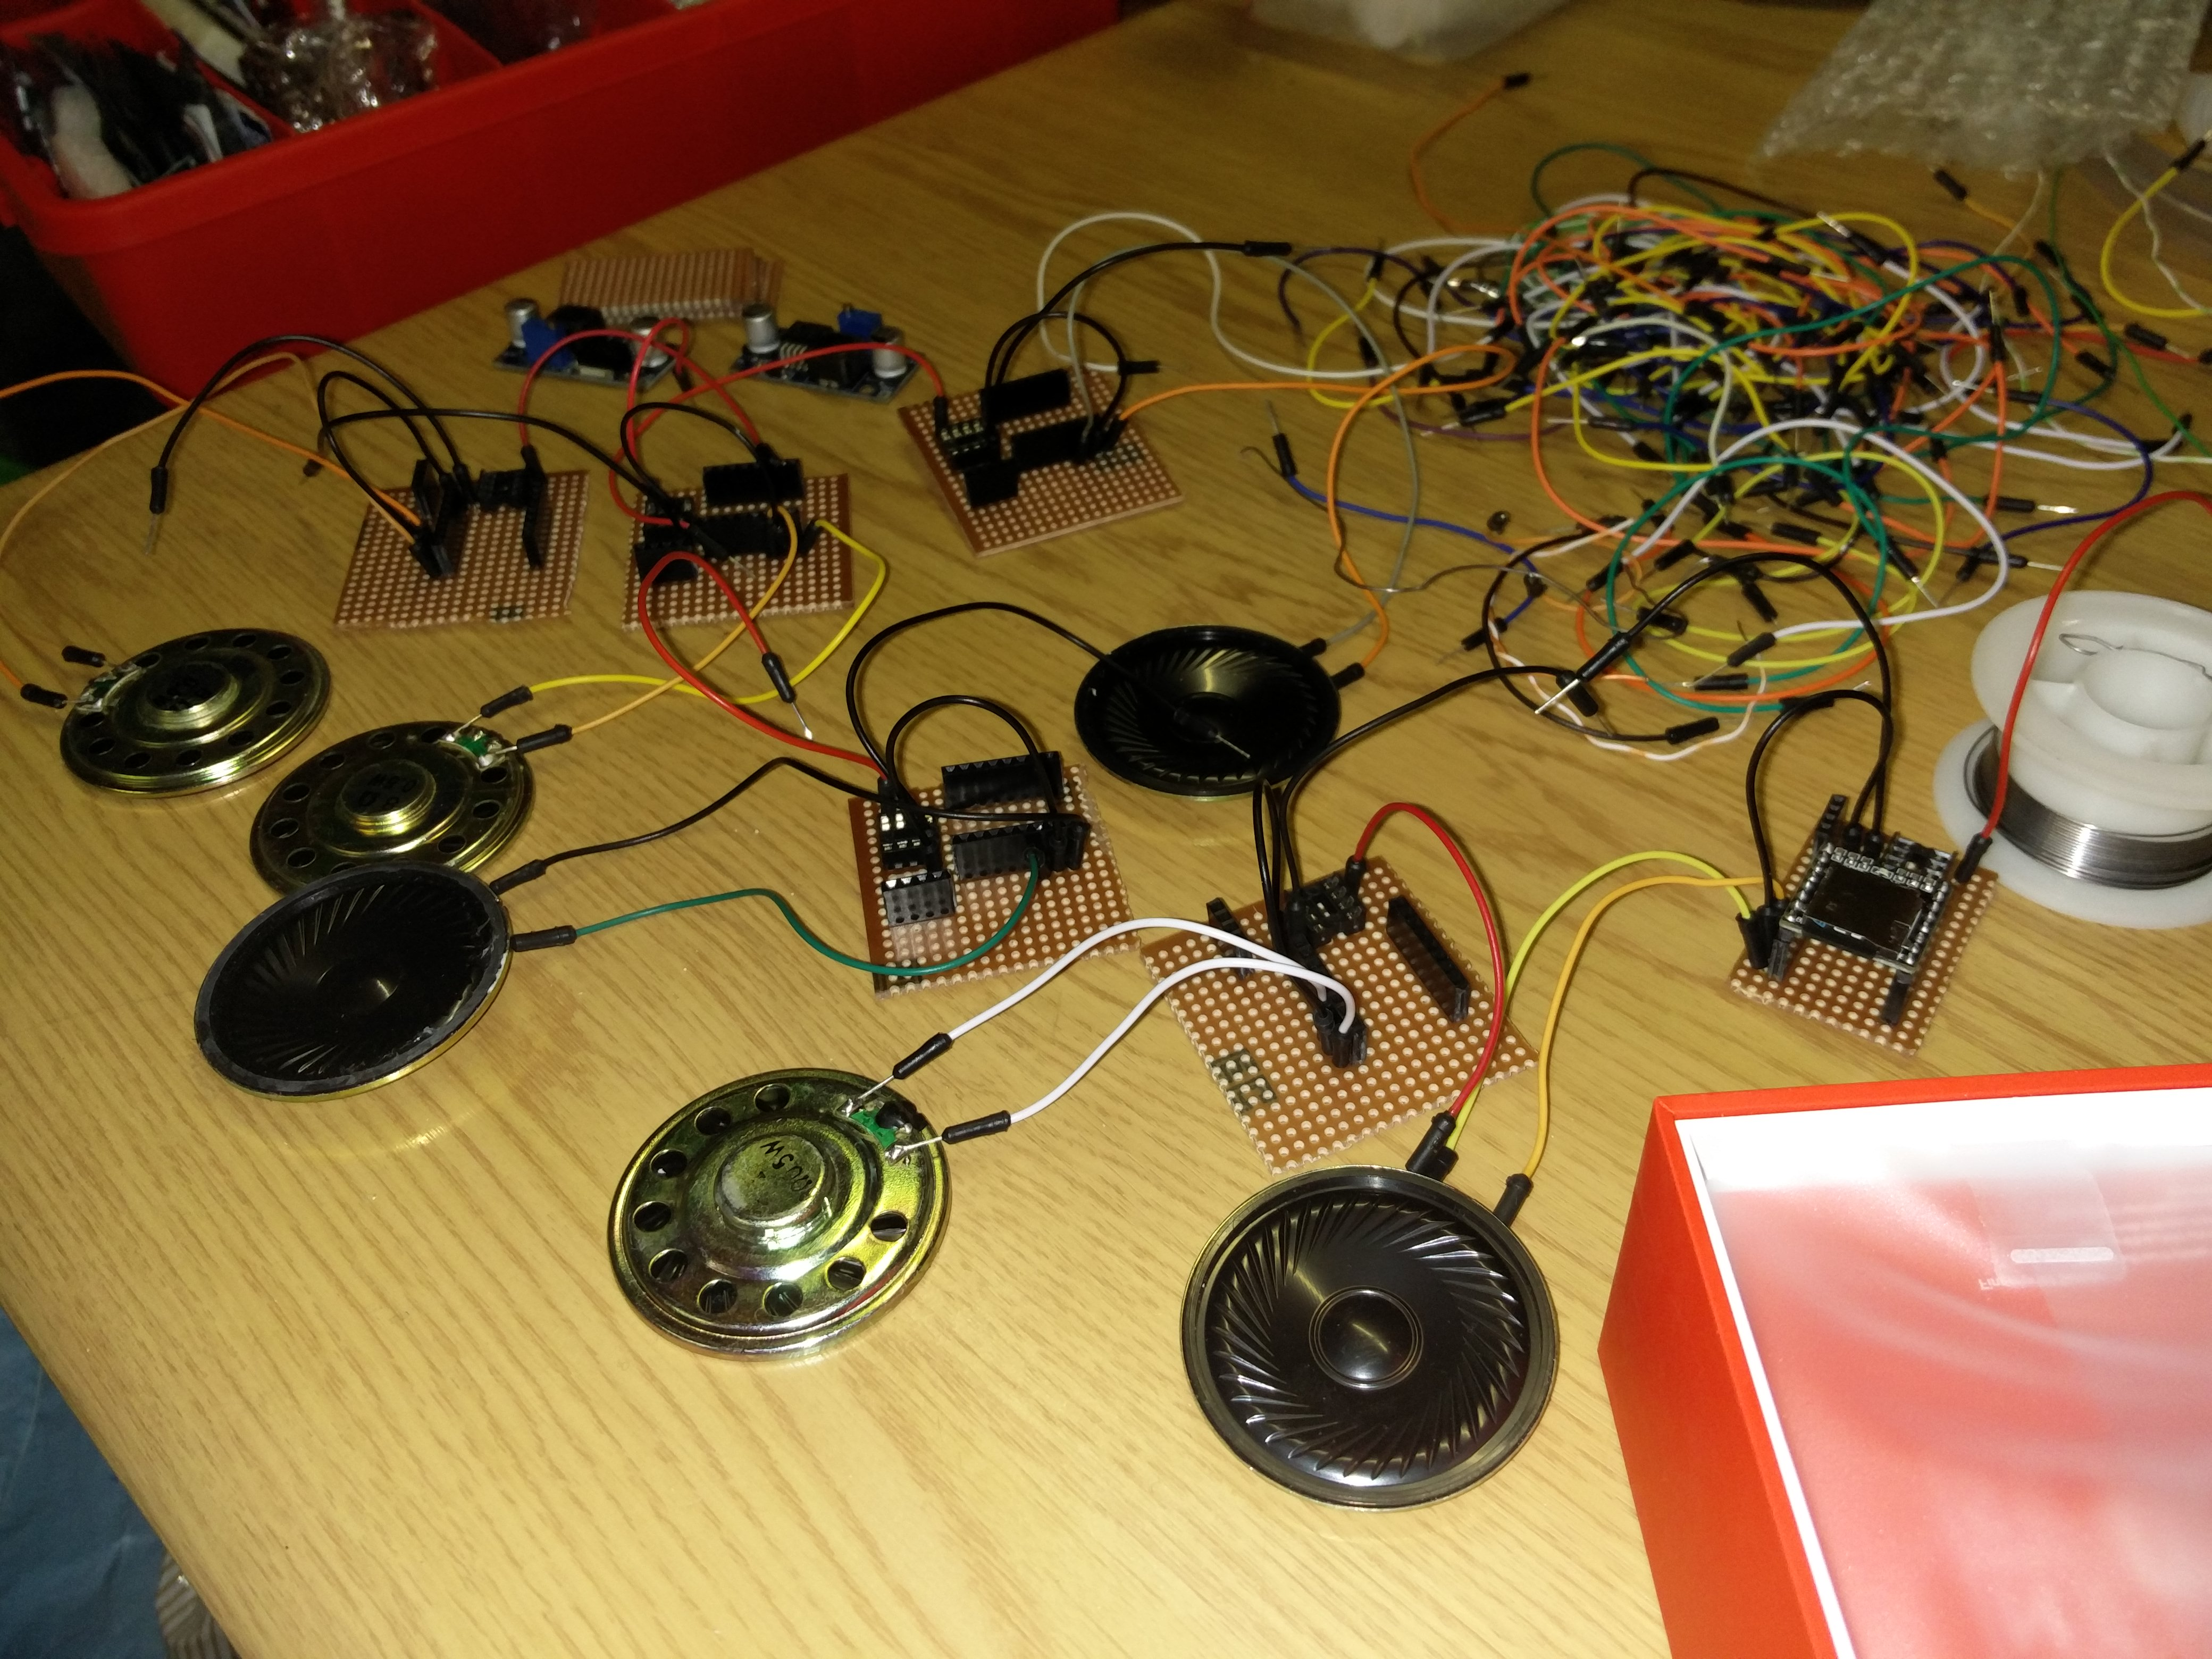
\includegraphics[width = 1.3in]{images/trash_1}} &    \subfloat[Trash Talk]{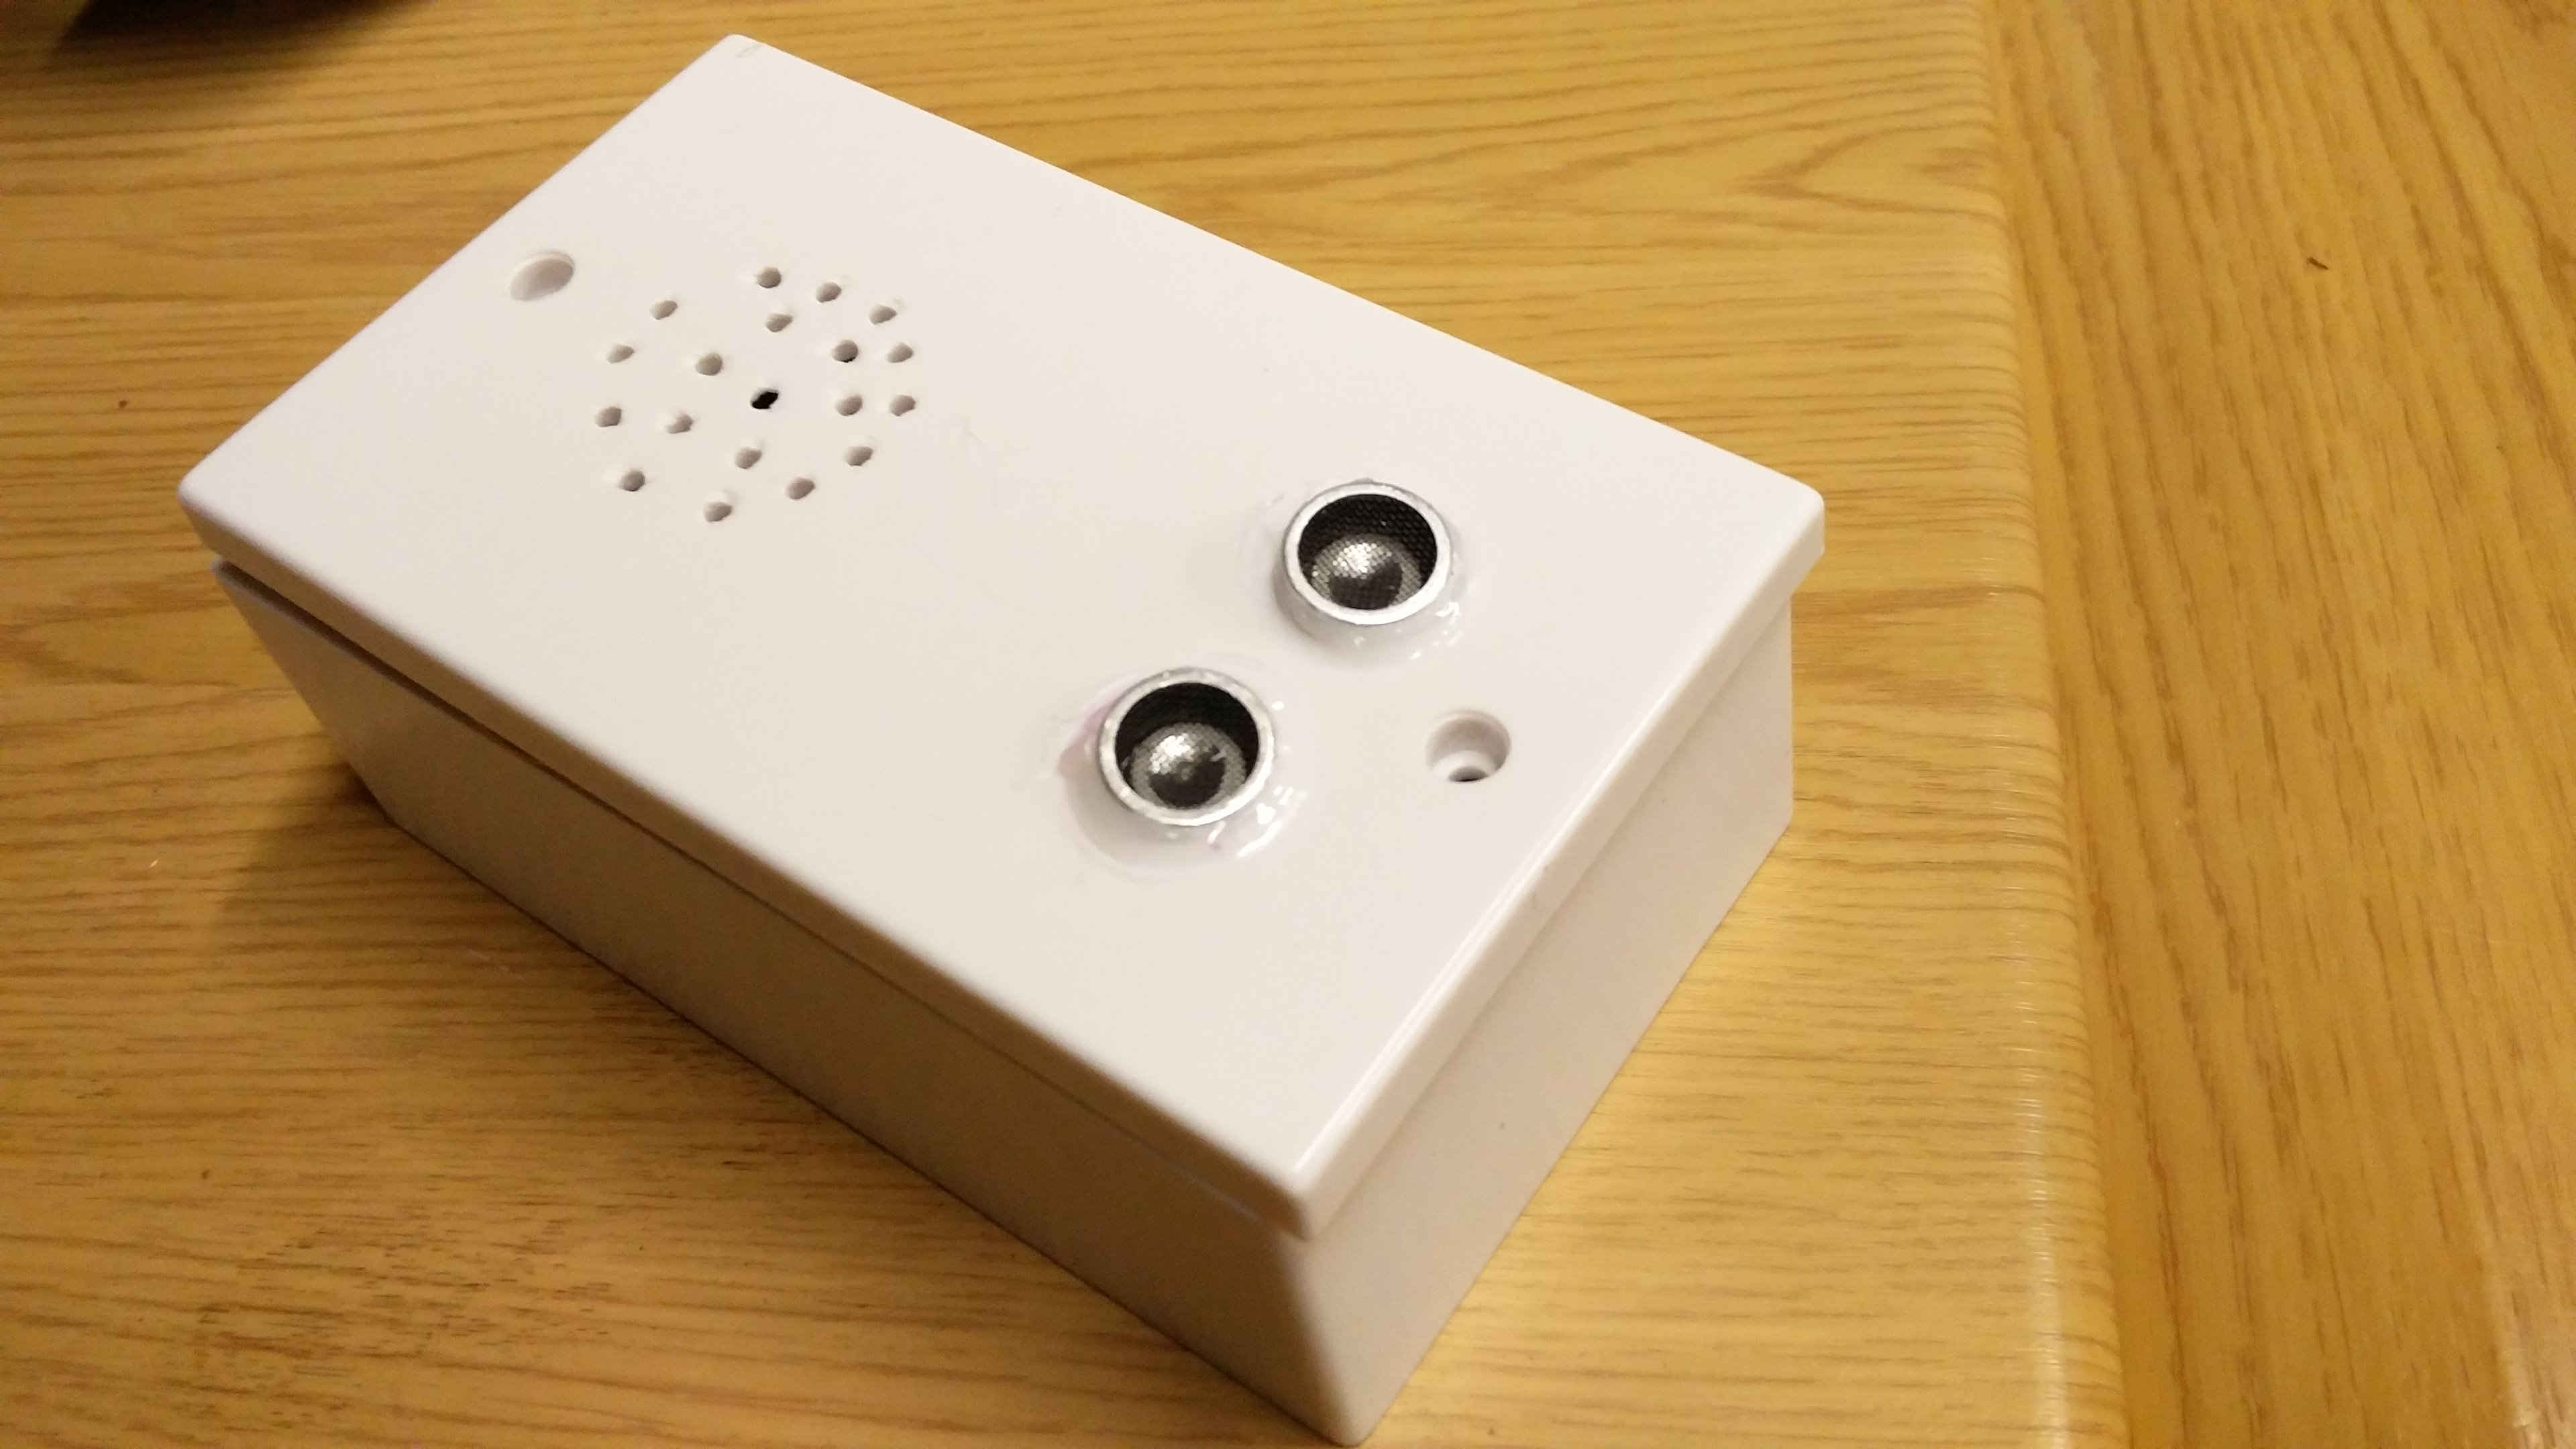
\includegraphics[width = 1.3in]{images/trash_2}} &
			\subfloat{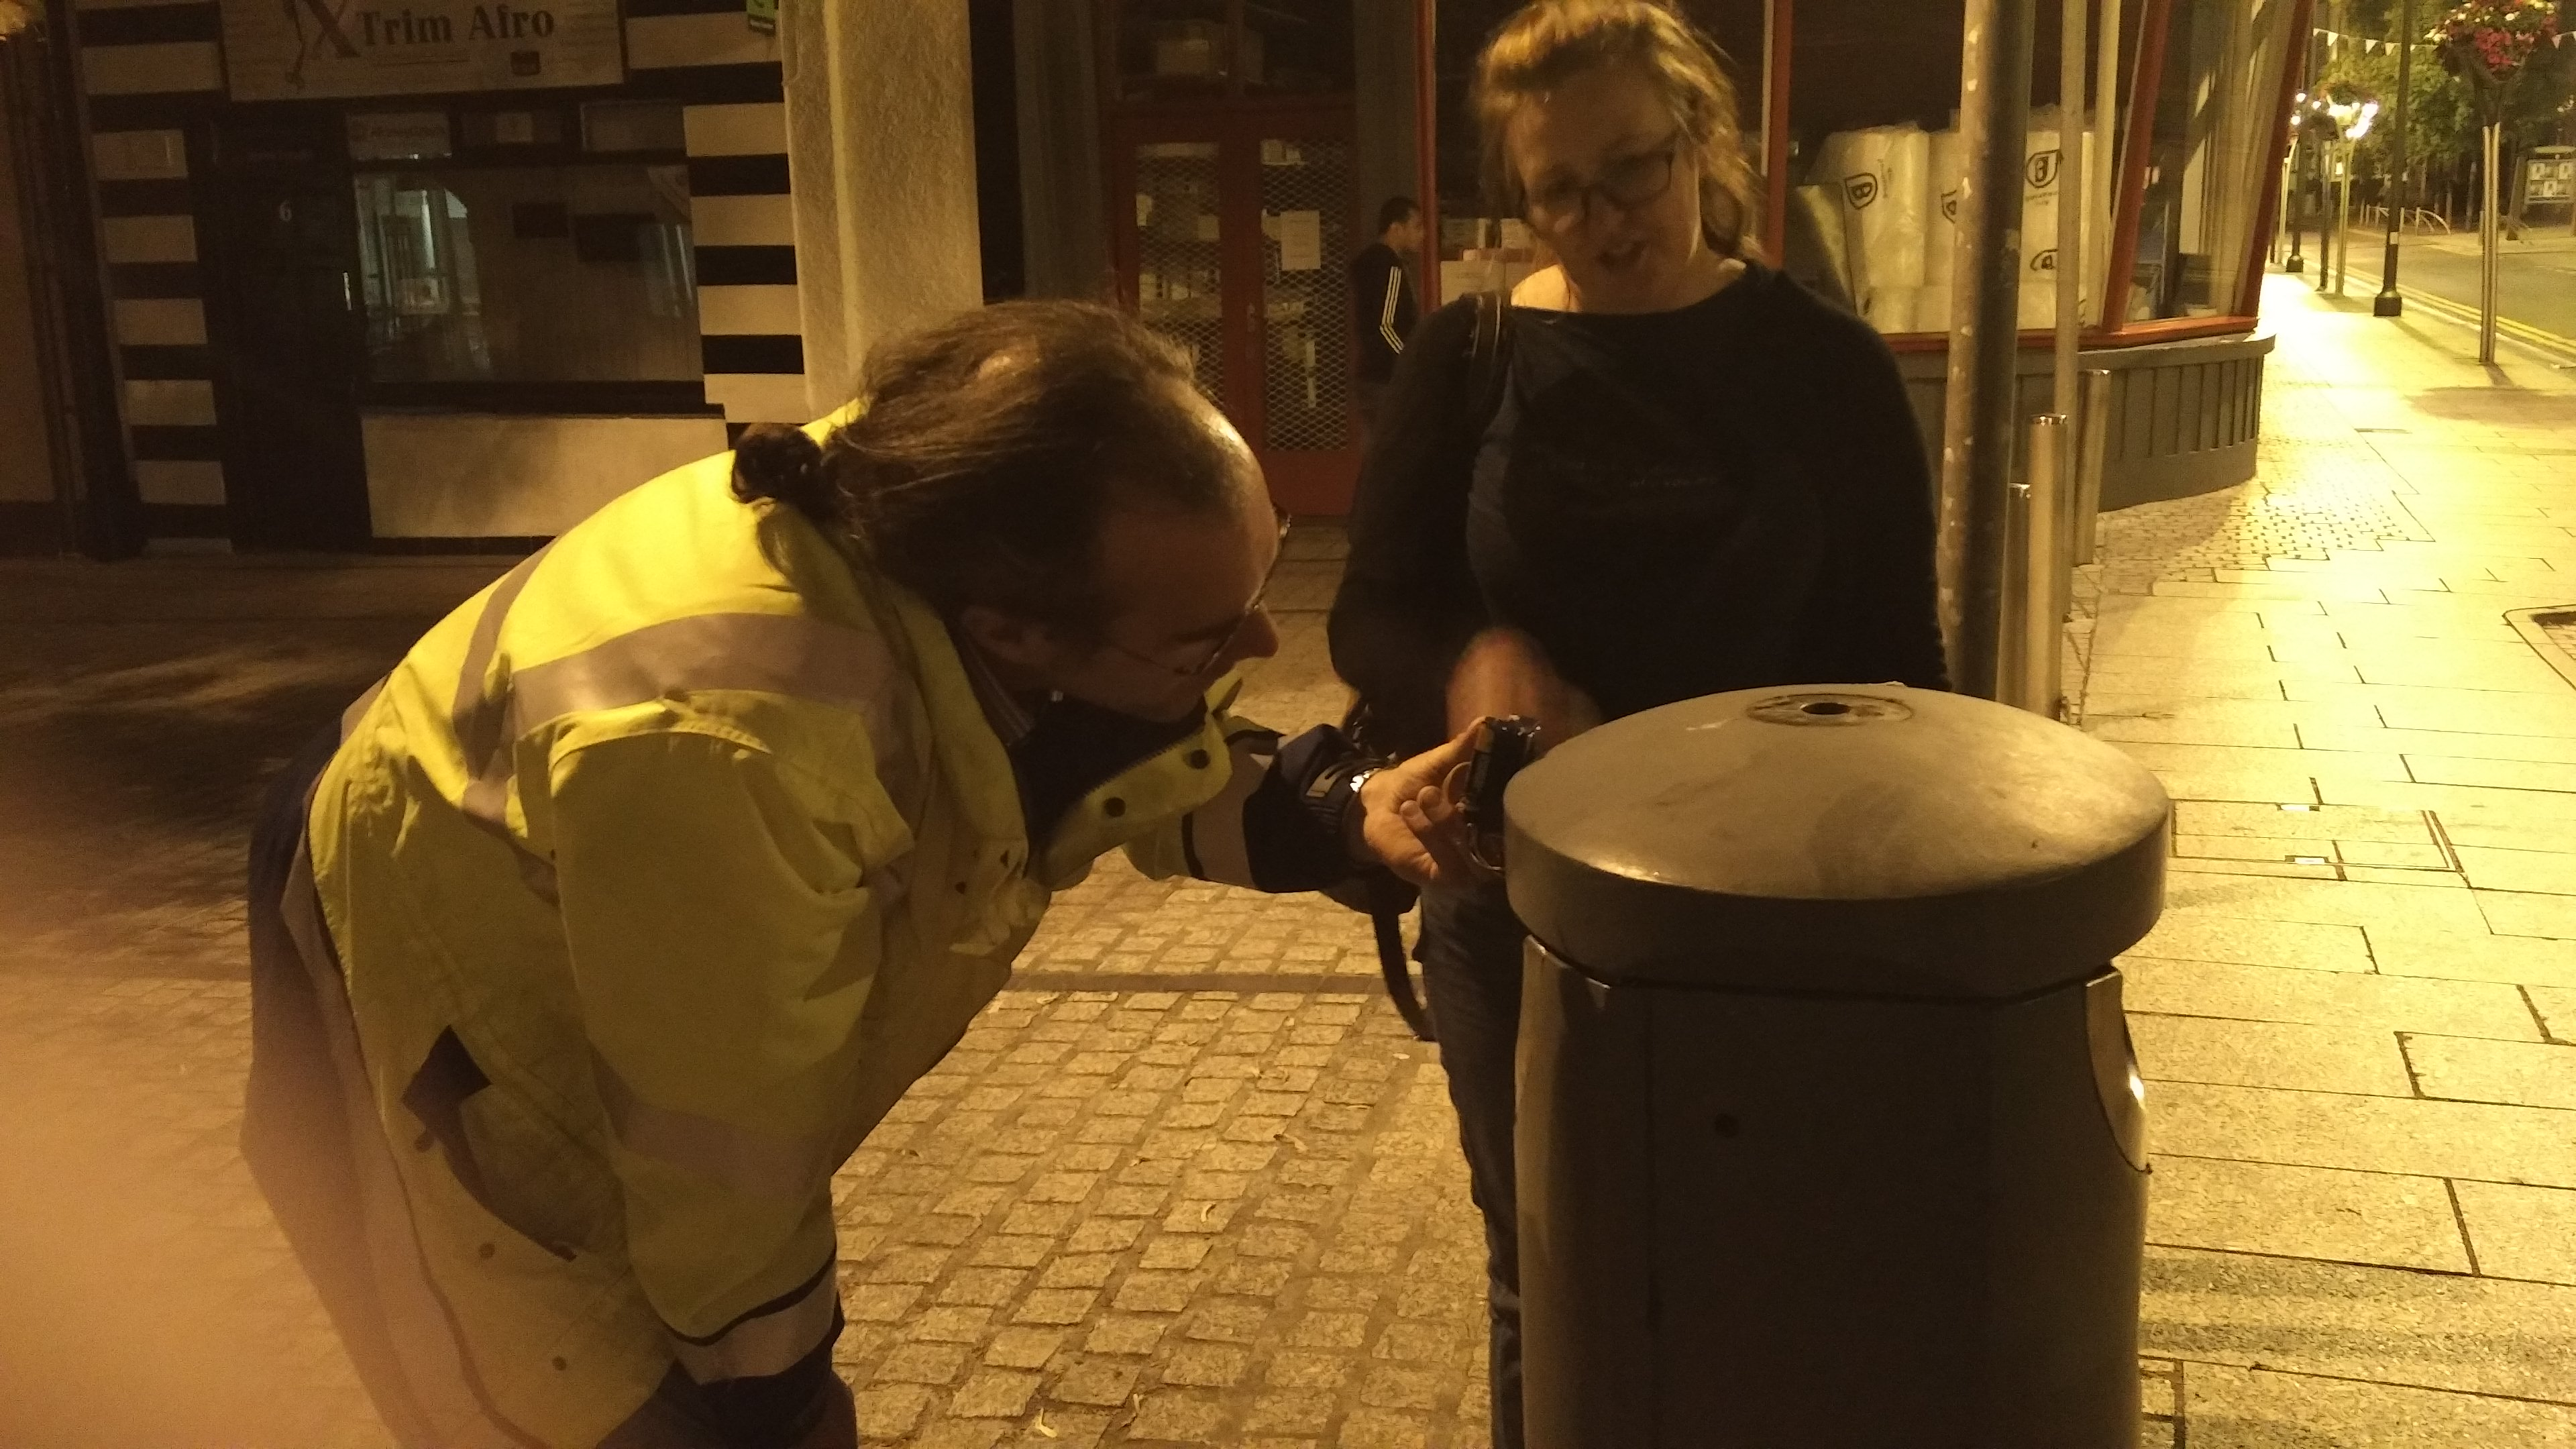
\includegraphics[width = 1.3in]{images/trash_3}} 
		\end{tabular}
		\caption{Digistreets at the Imagine Arts Festival Waterford 2016}
	\end{figure}
\end{frame}


\section{Floppy Drive MIDI Player}
\begin{frame}{Floppy Drive MIDI Player}
	\begin{figure}
		\begin{tabular}{ccc}
			\subfloat{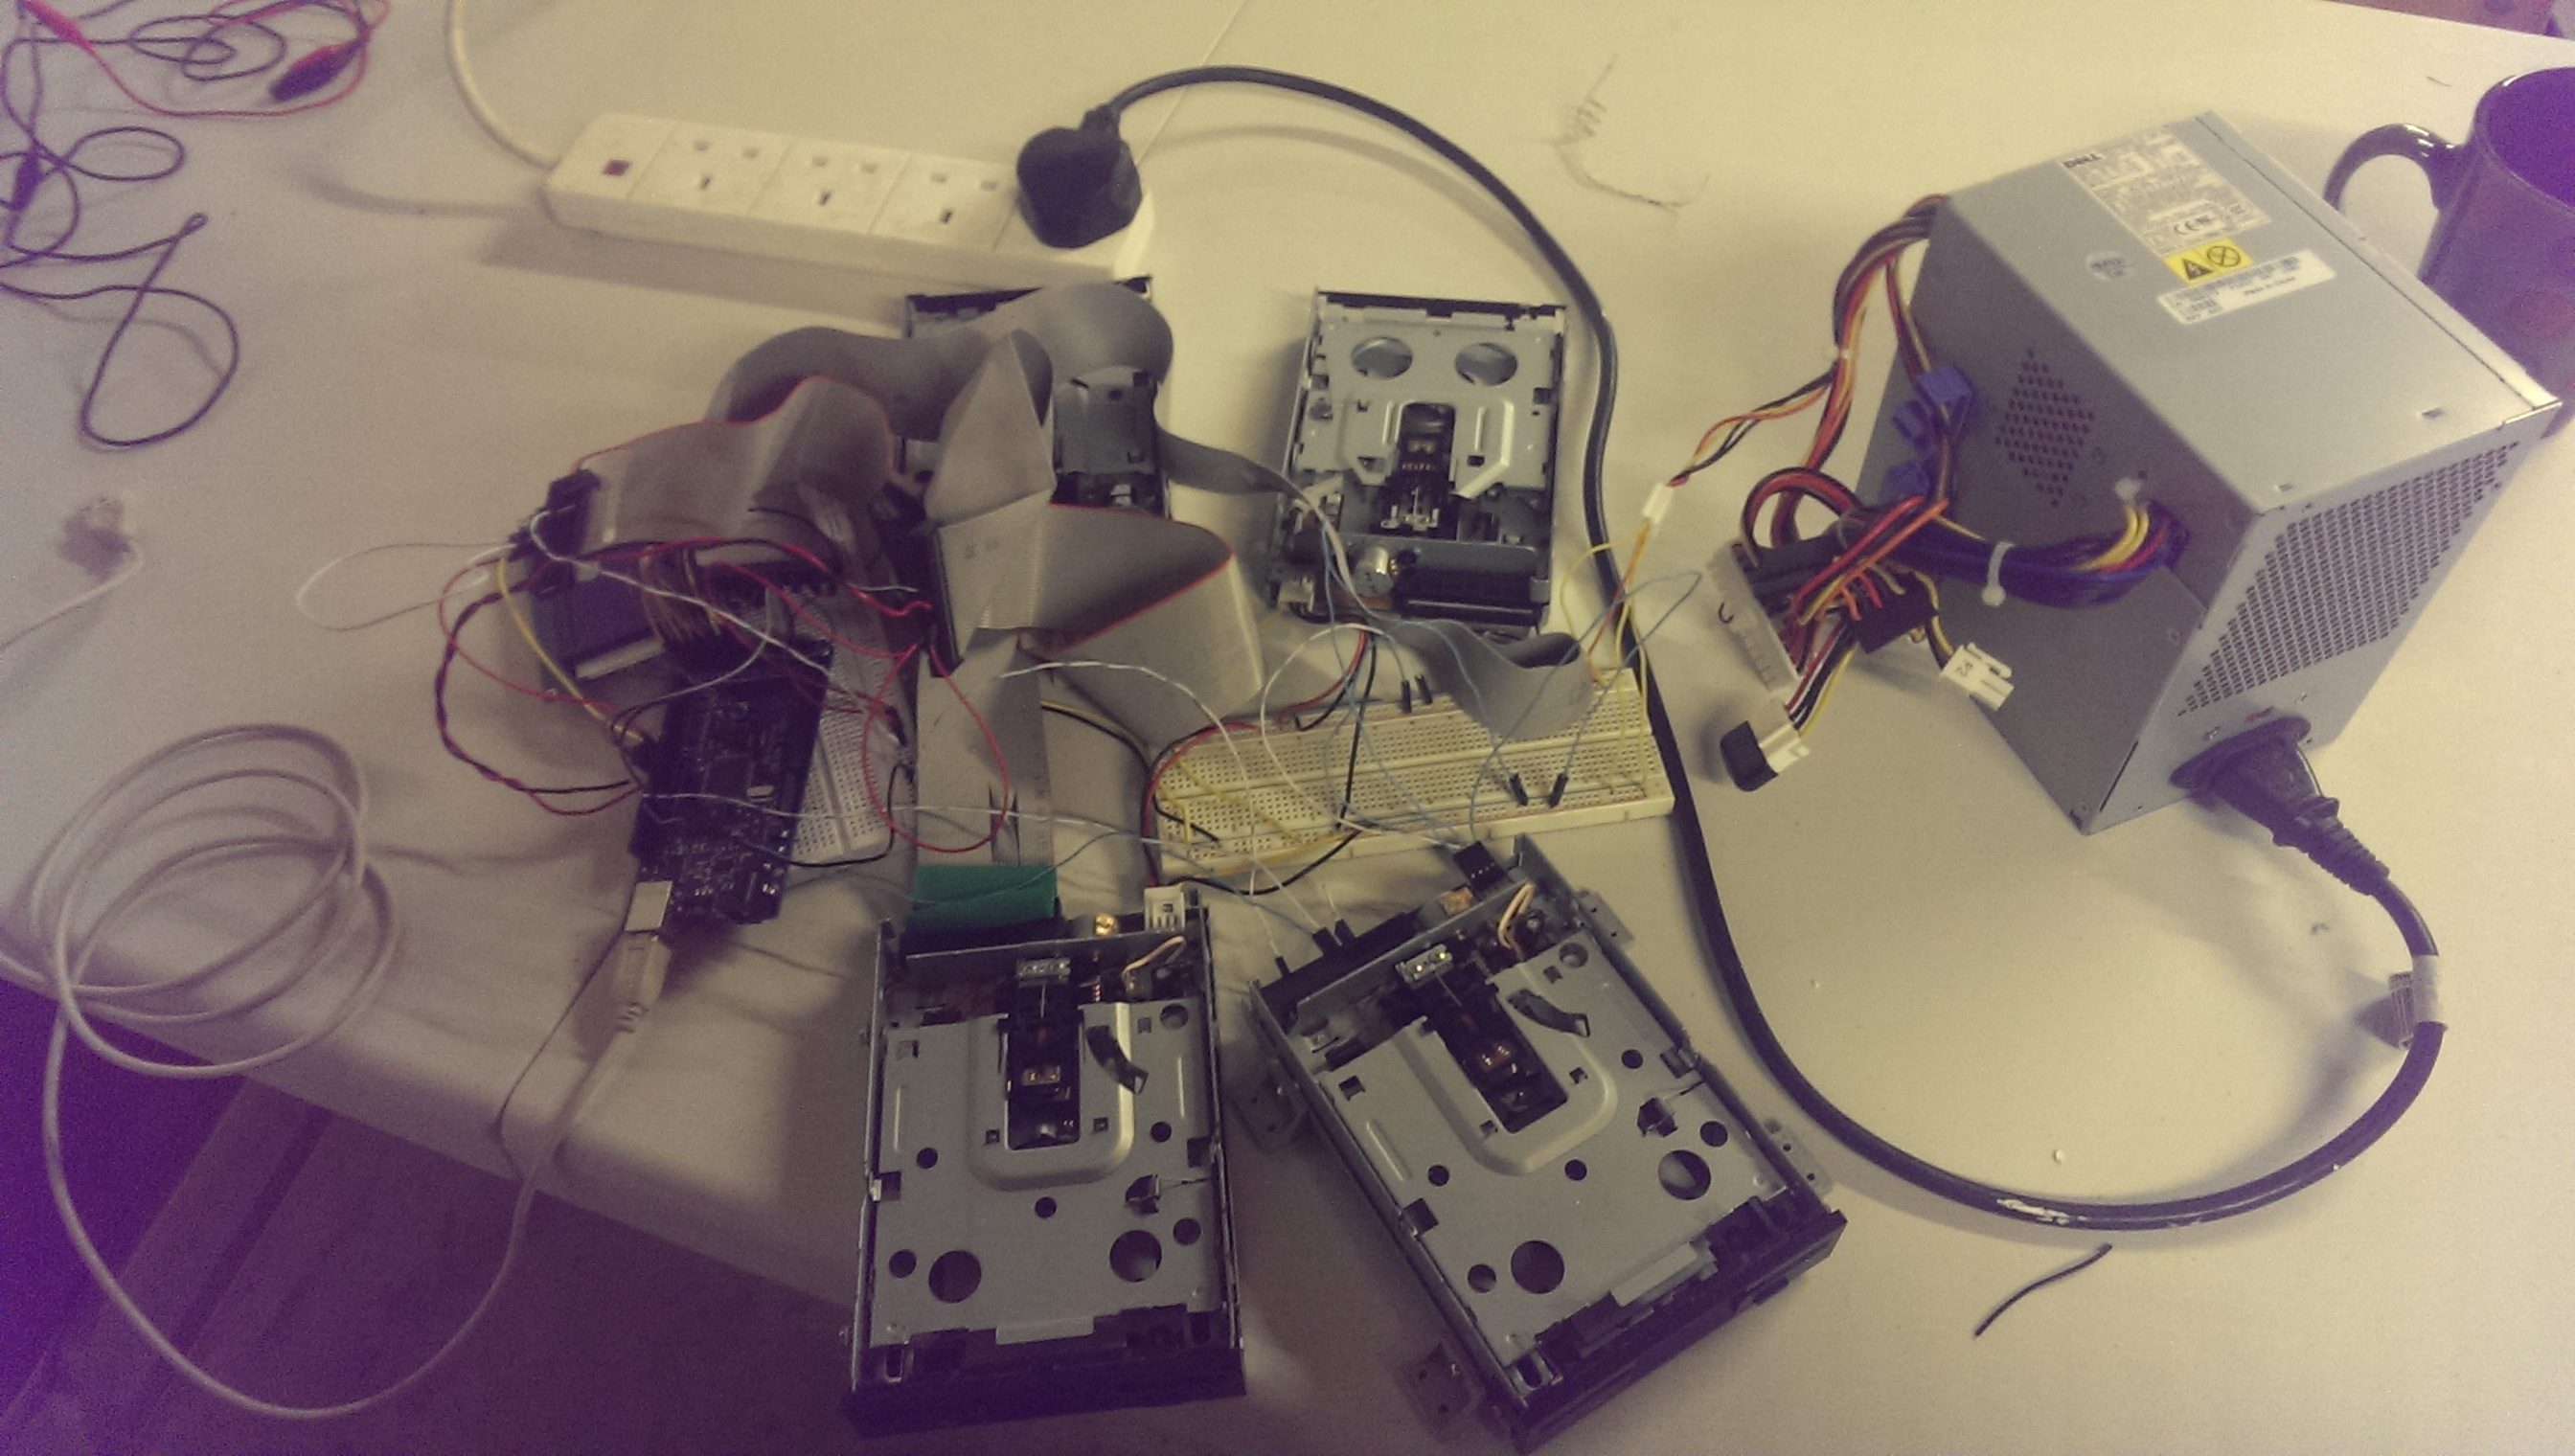
\includegraphics[width = 1.3in]{images/floppy_1}} &
			\subfloat{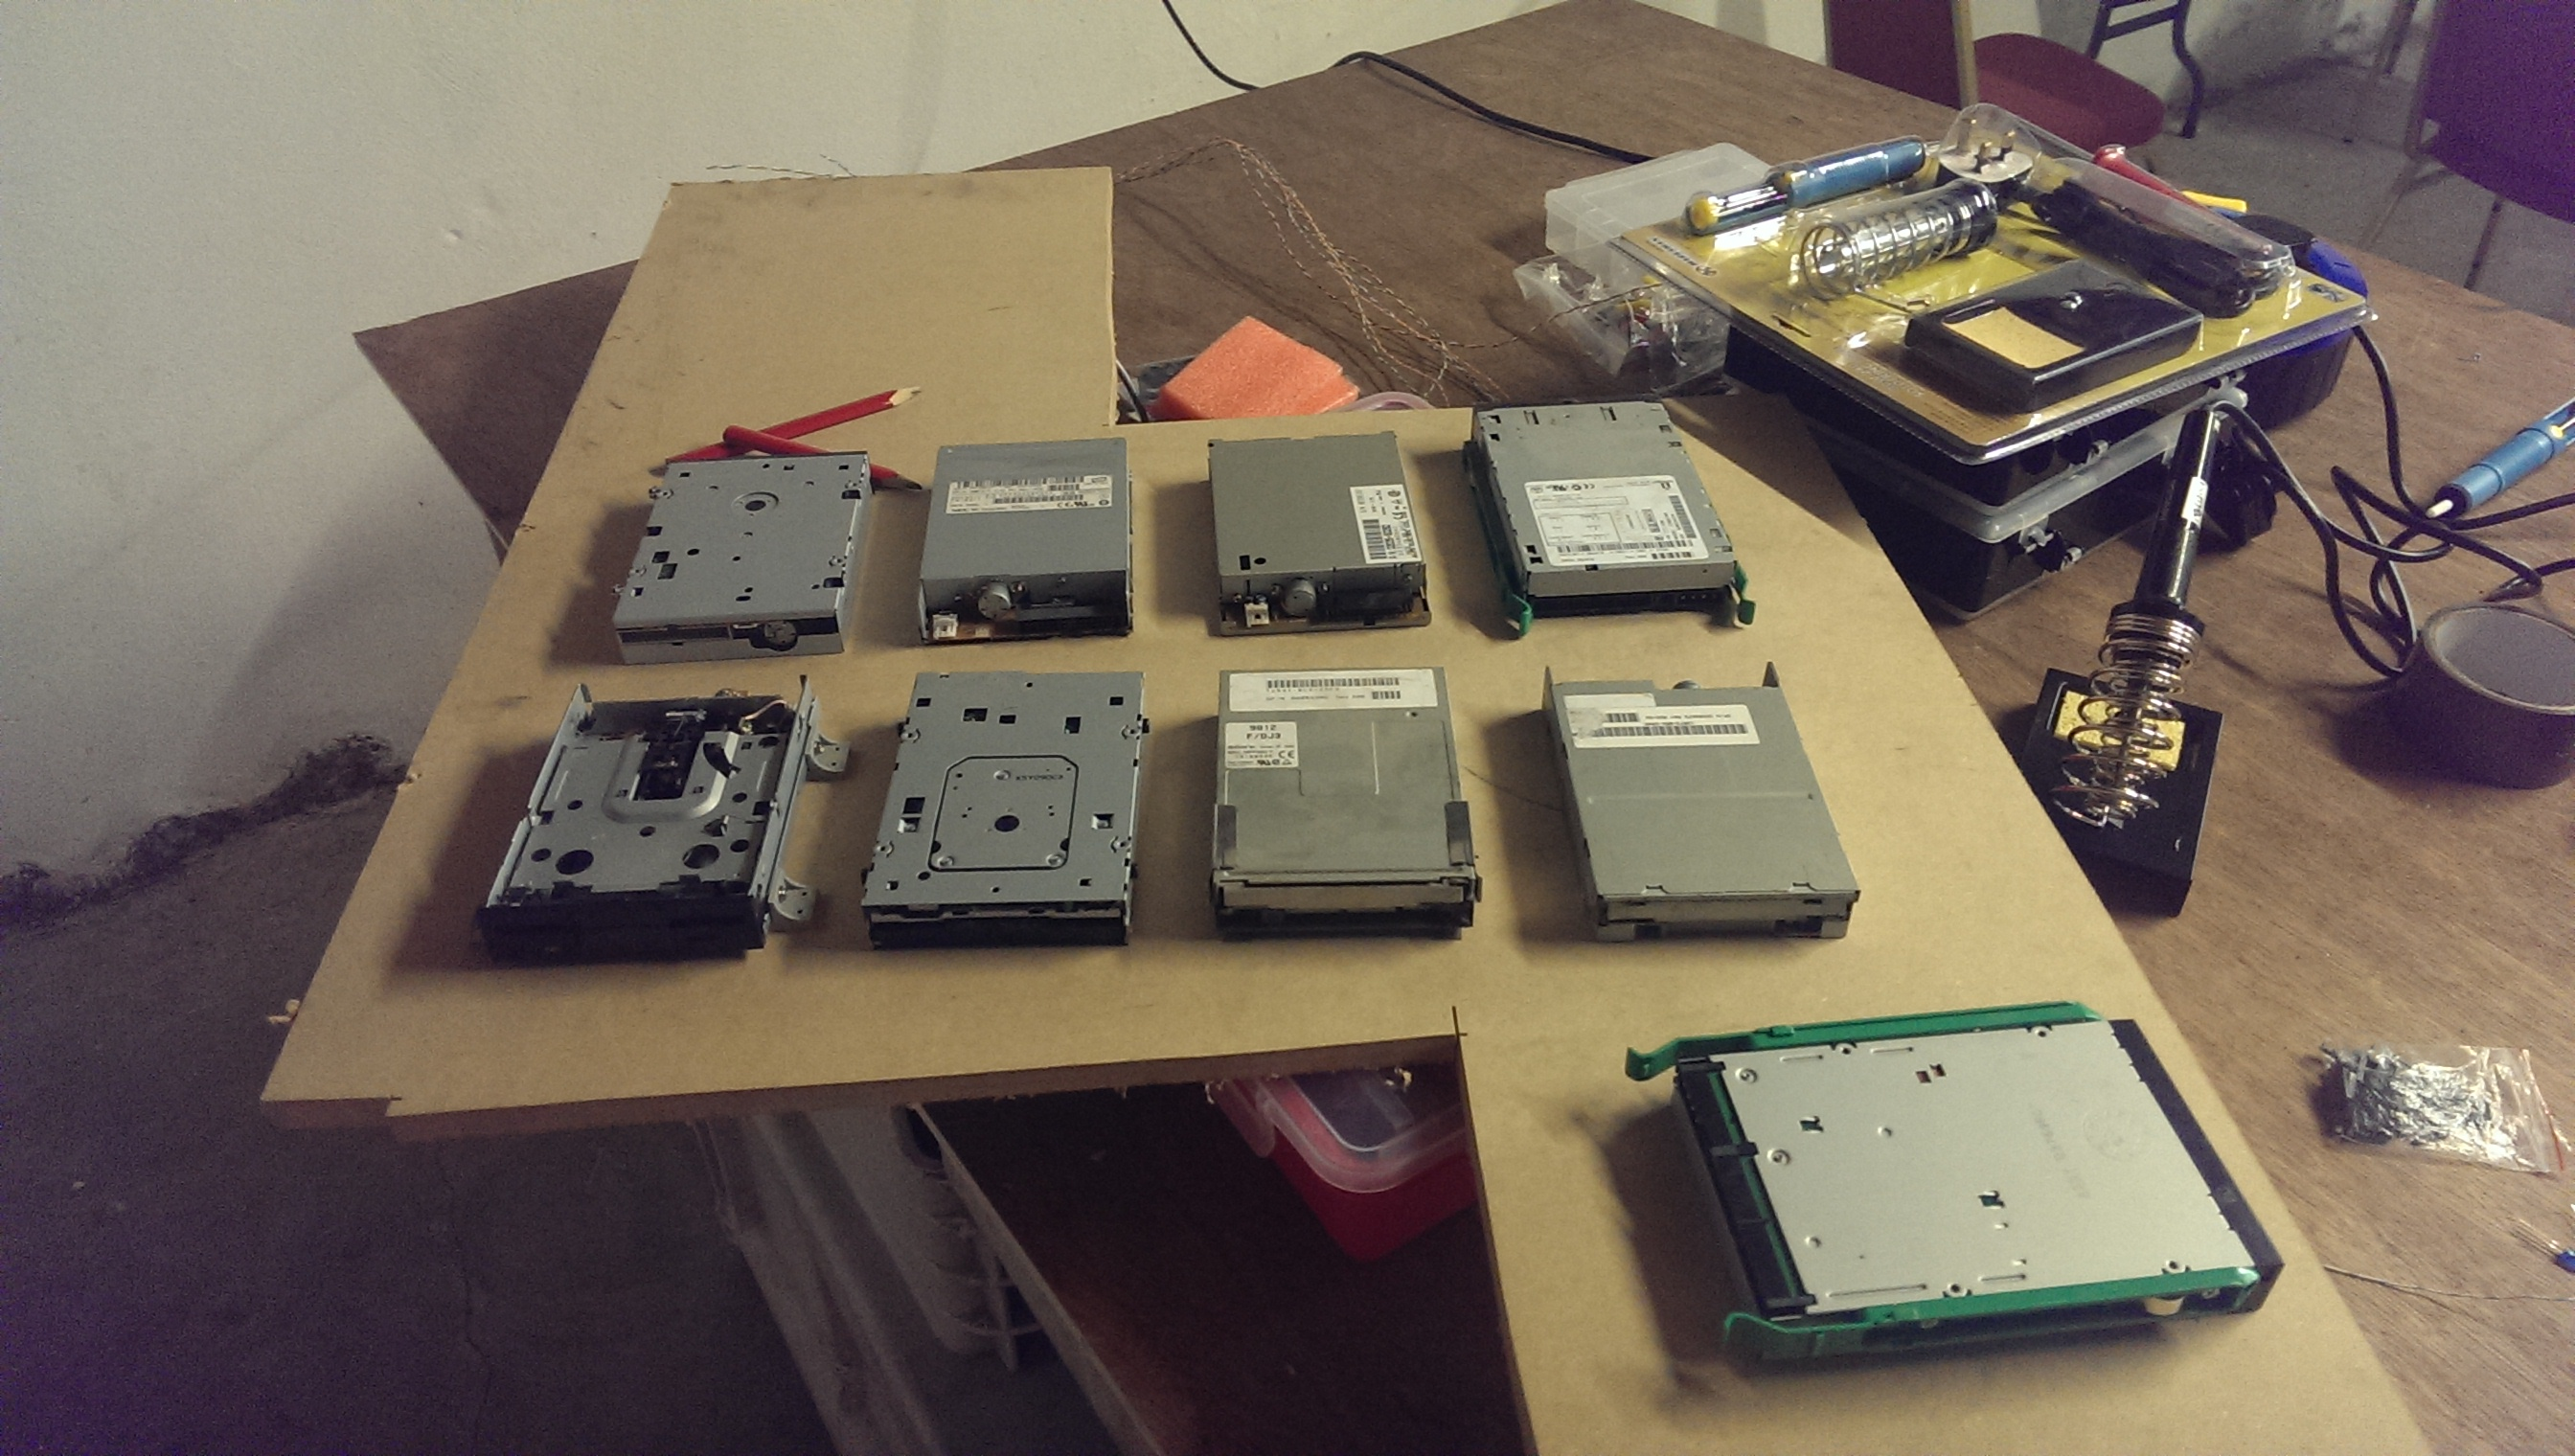
\includegraphics[width = 1.3in]{images/floppy_2}} &
			\subfloat{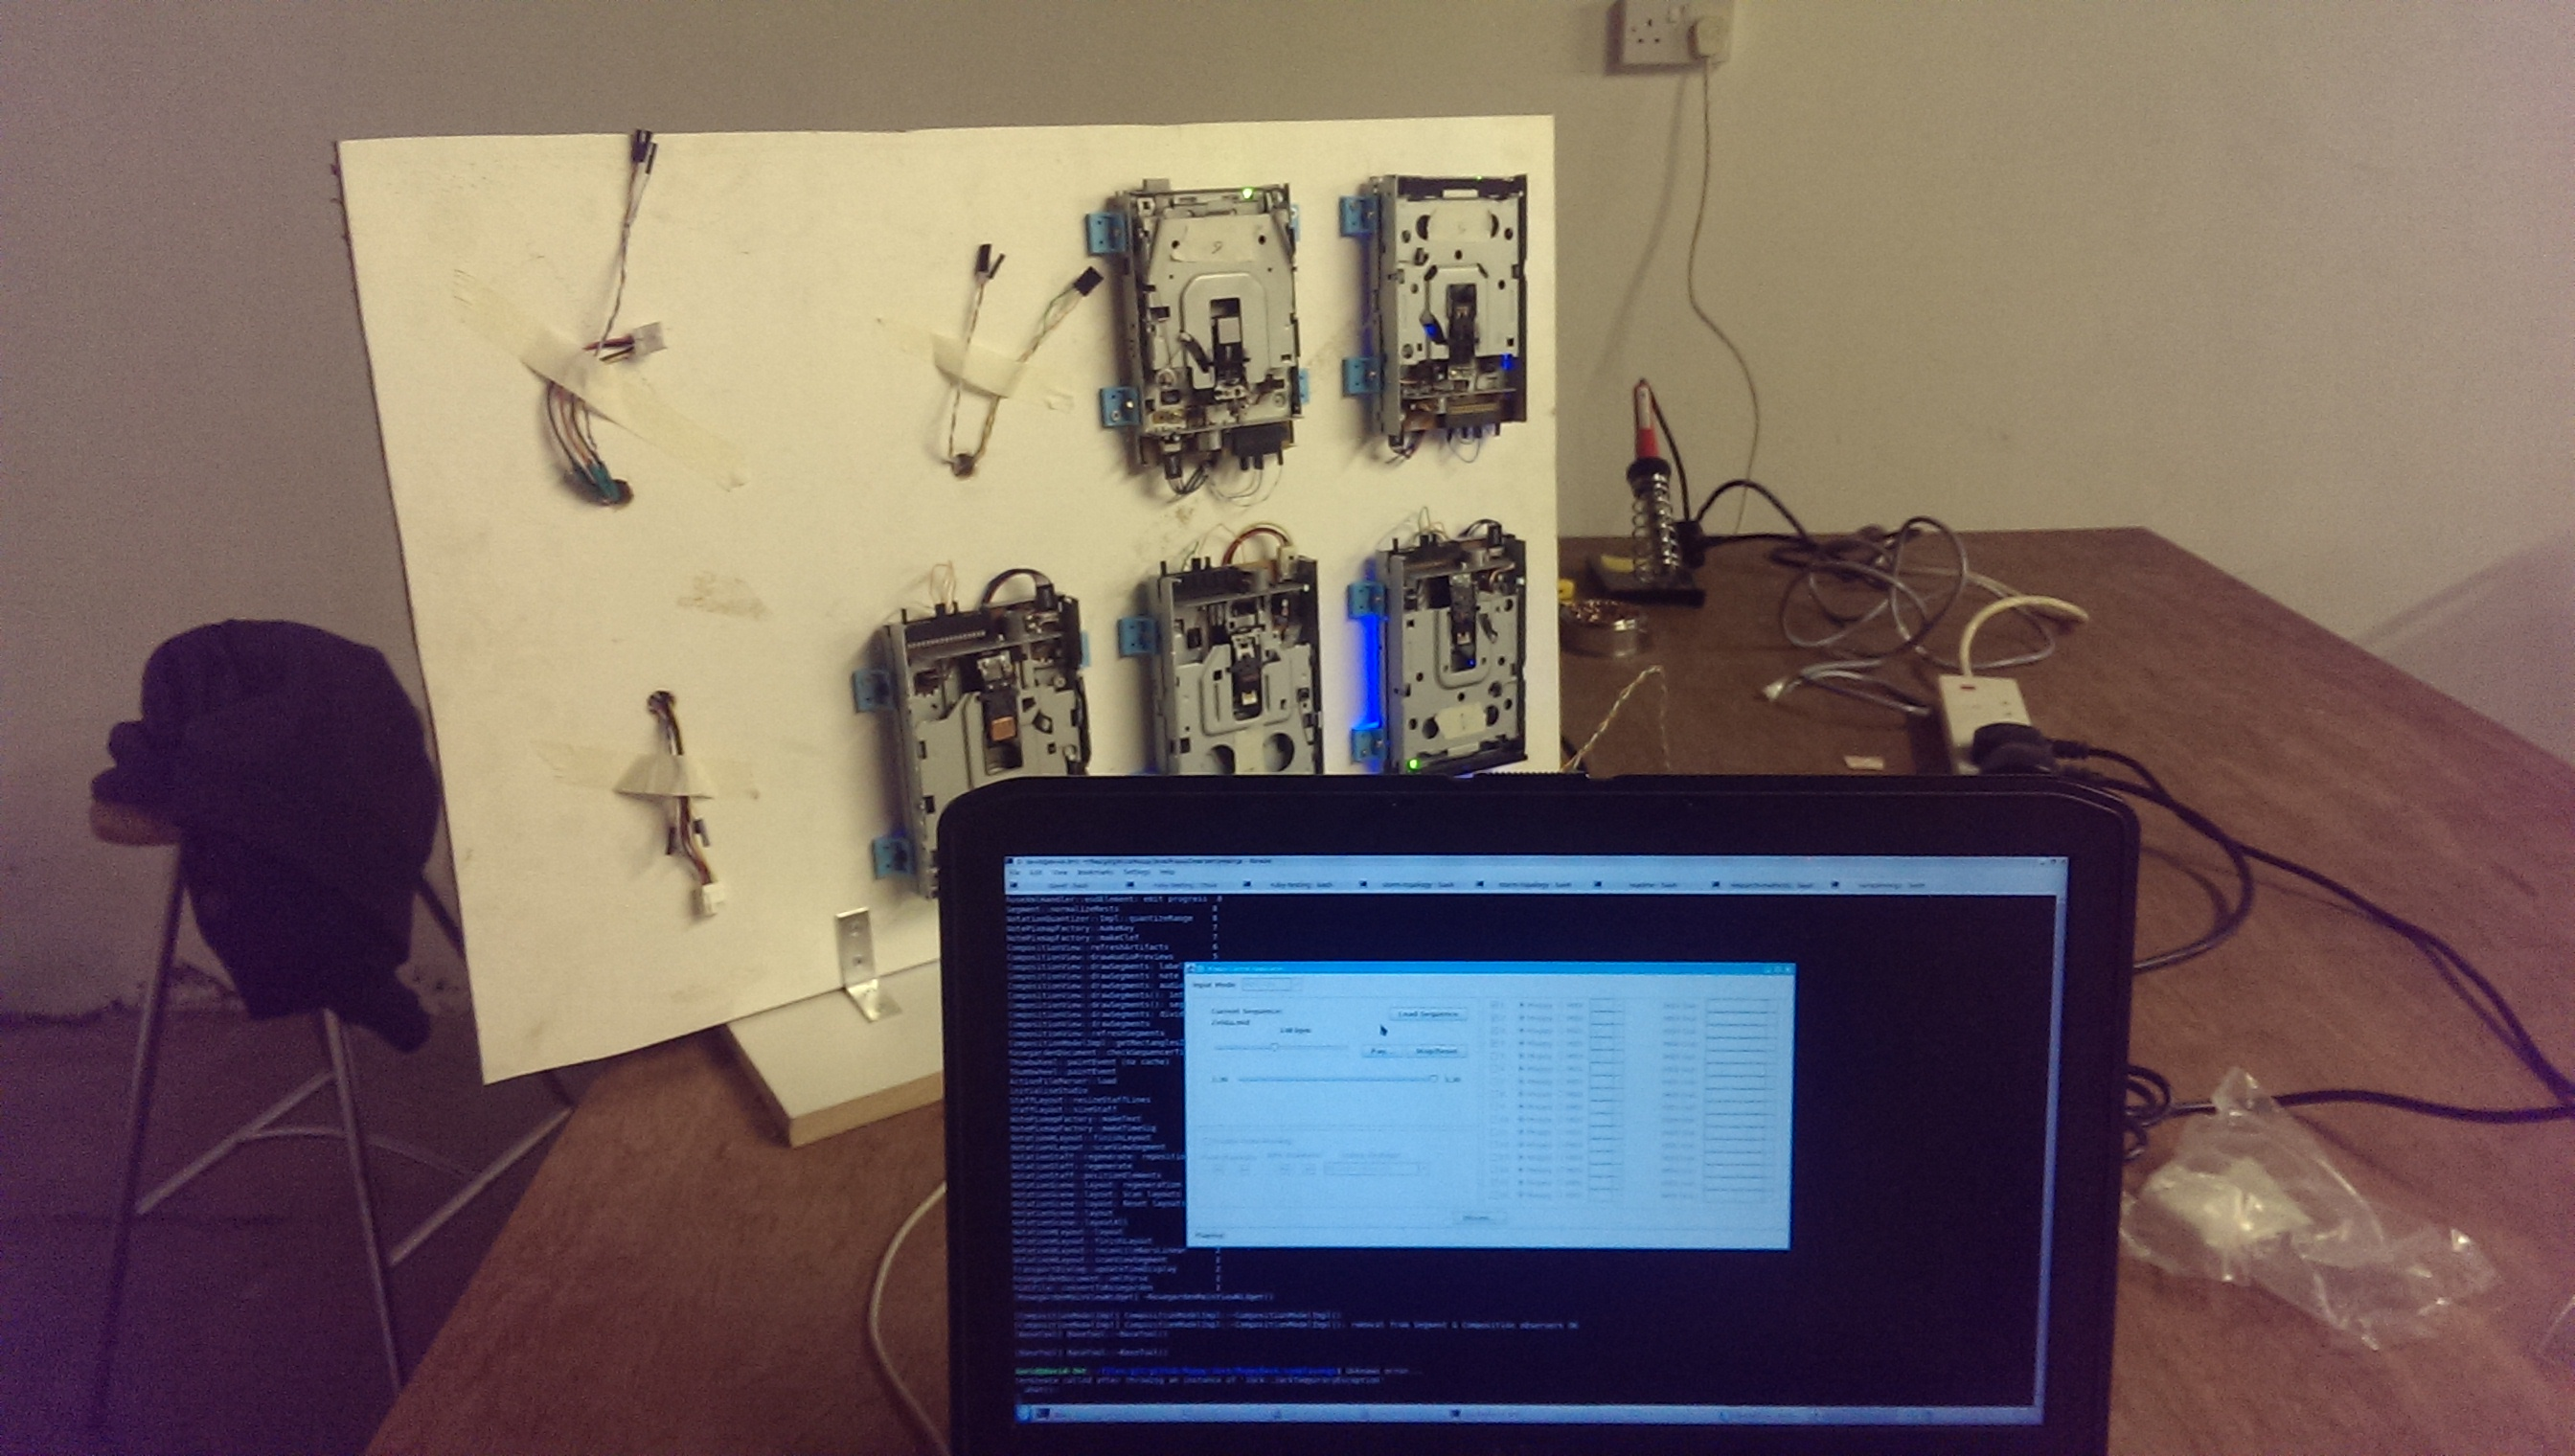
\includegraphics[width = 1.3in]{images/floppy_3}} \\
			\subfloat{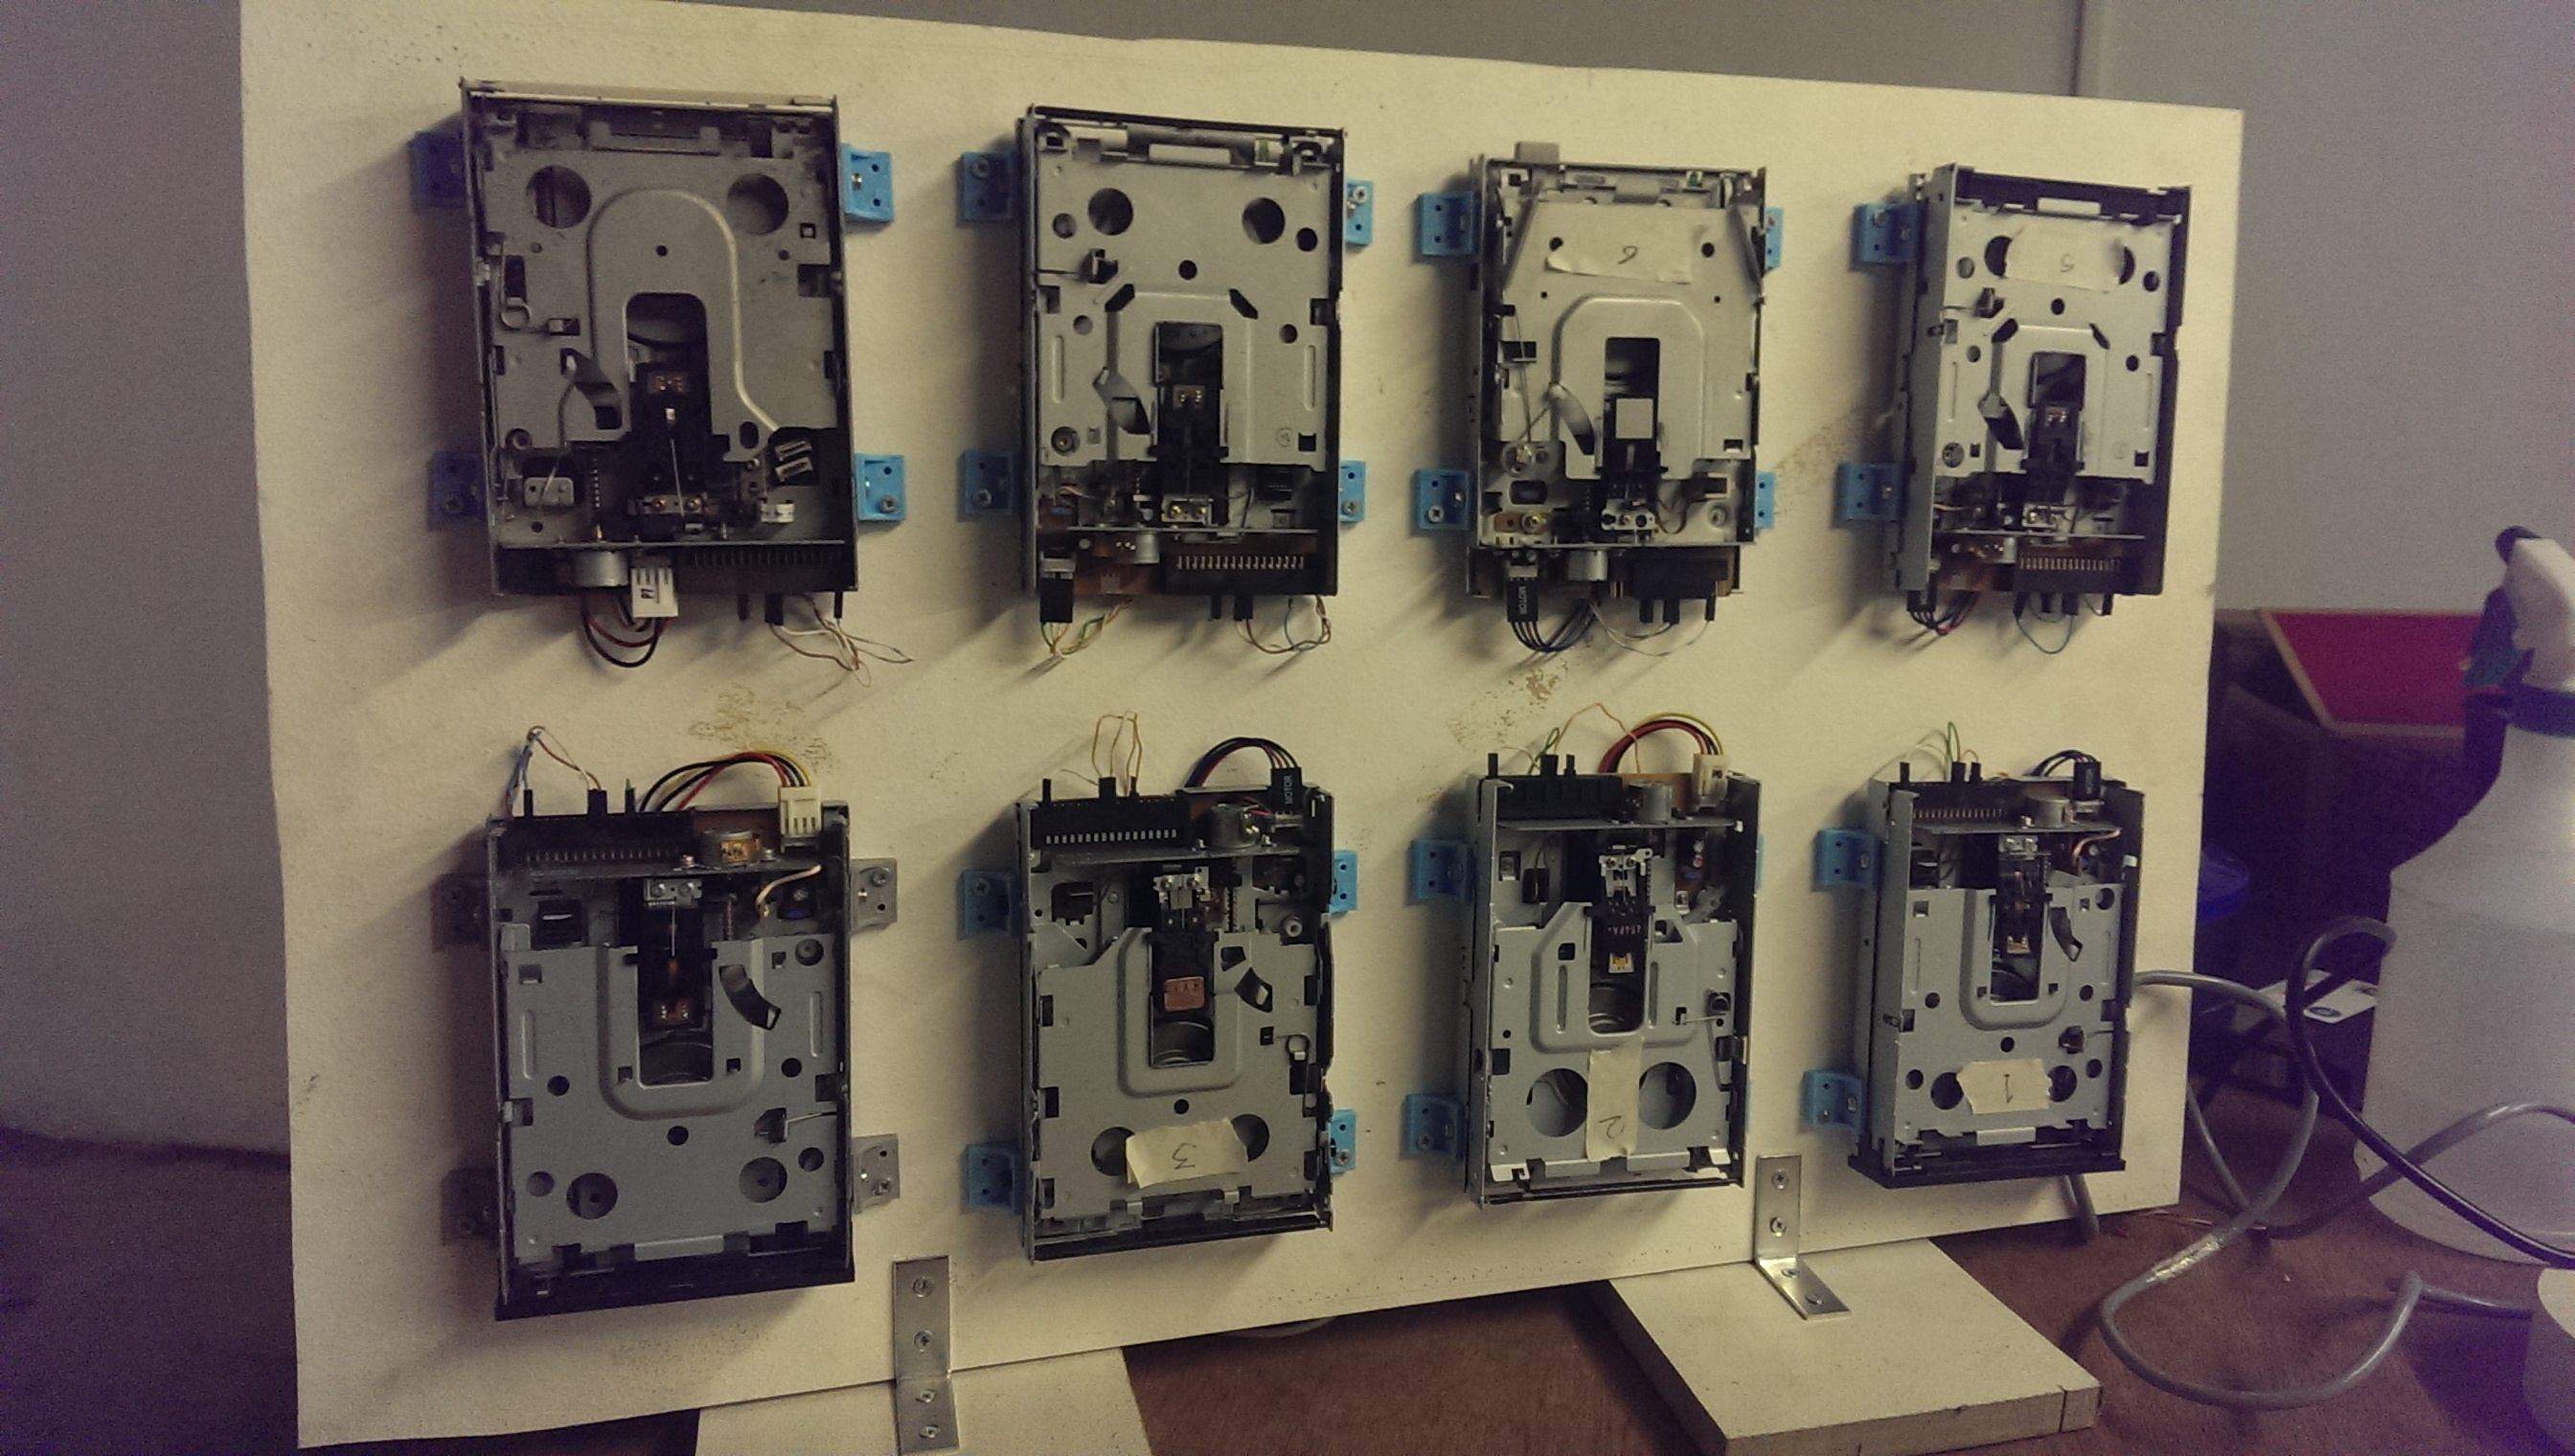
\includegraphics[width = 1.3in]{images/floppy_4}} &    \subfloat{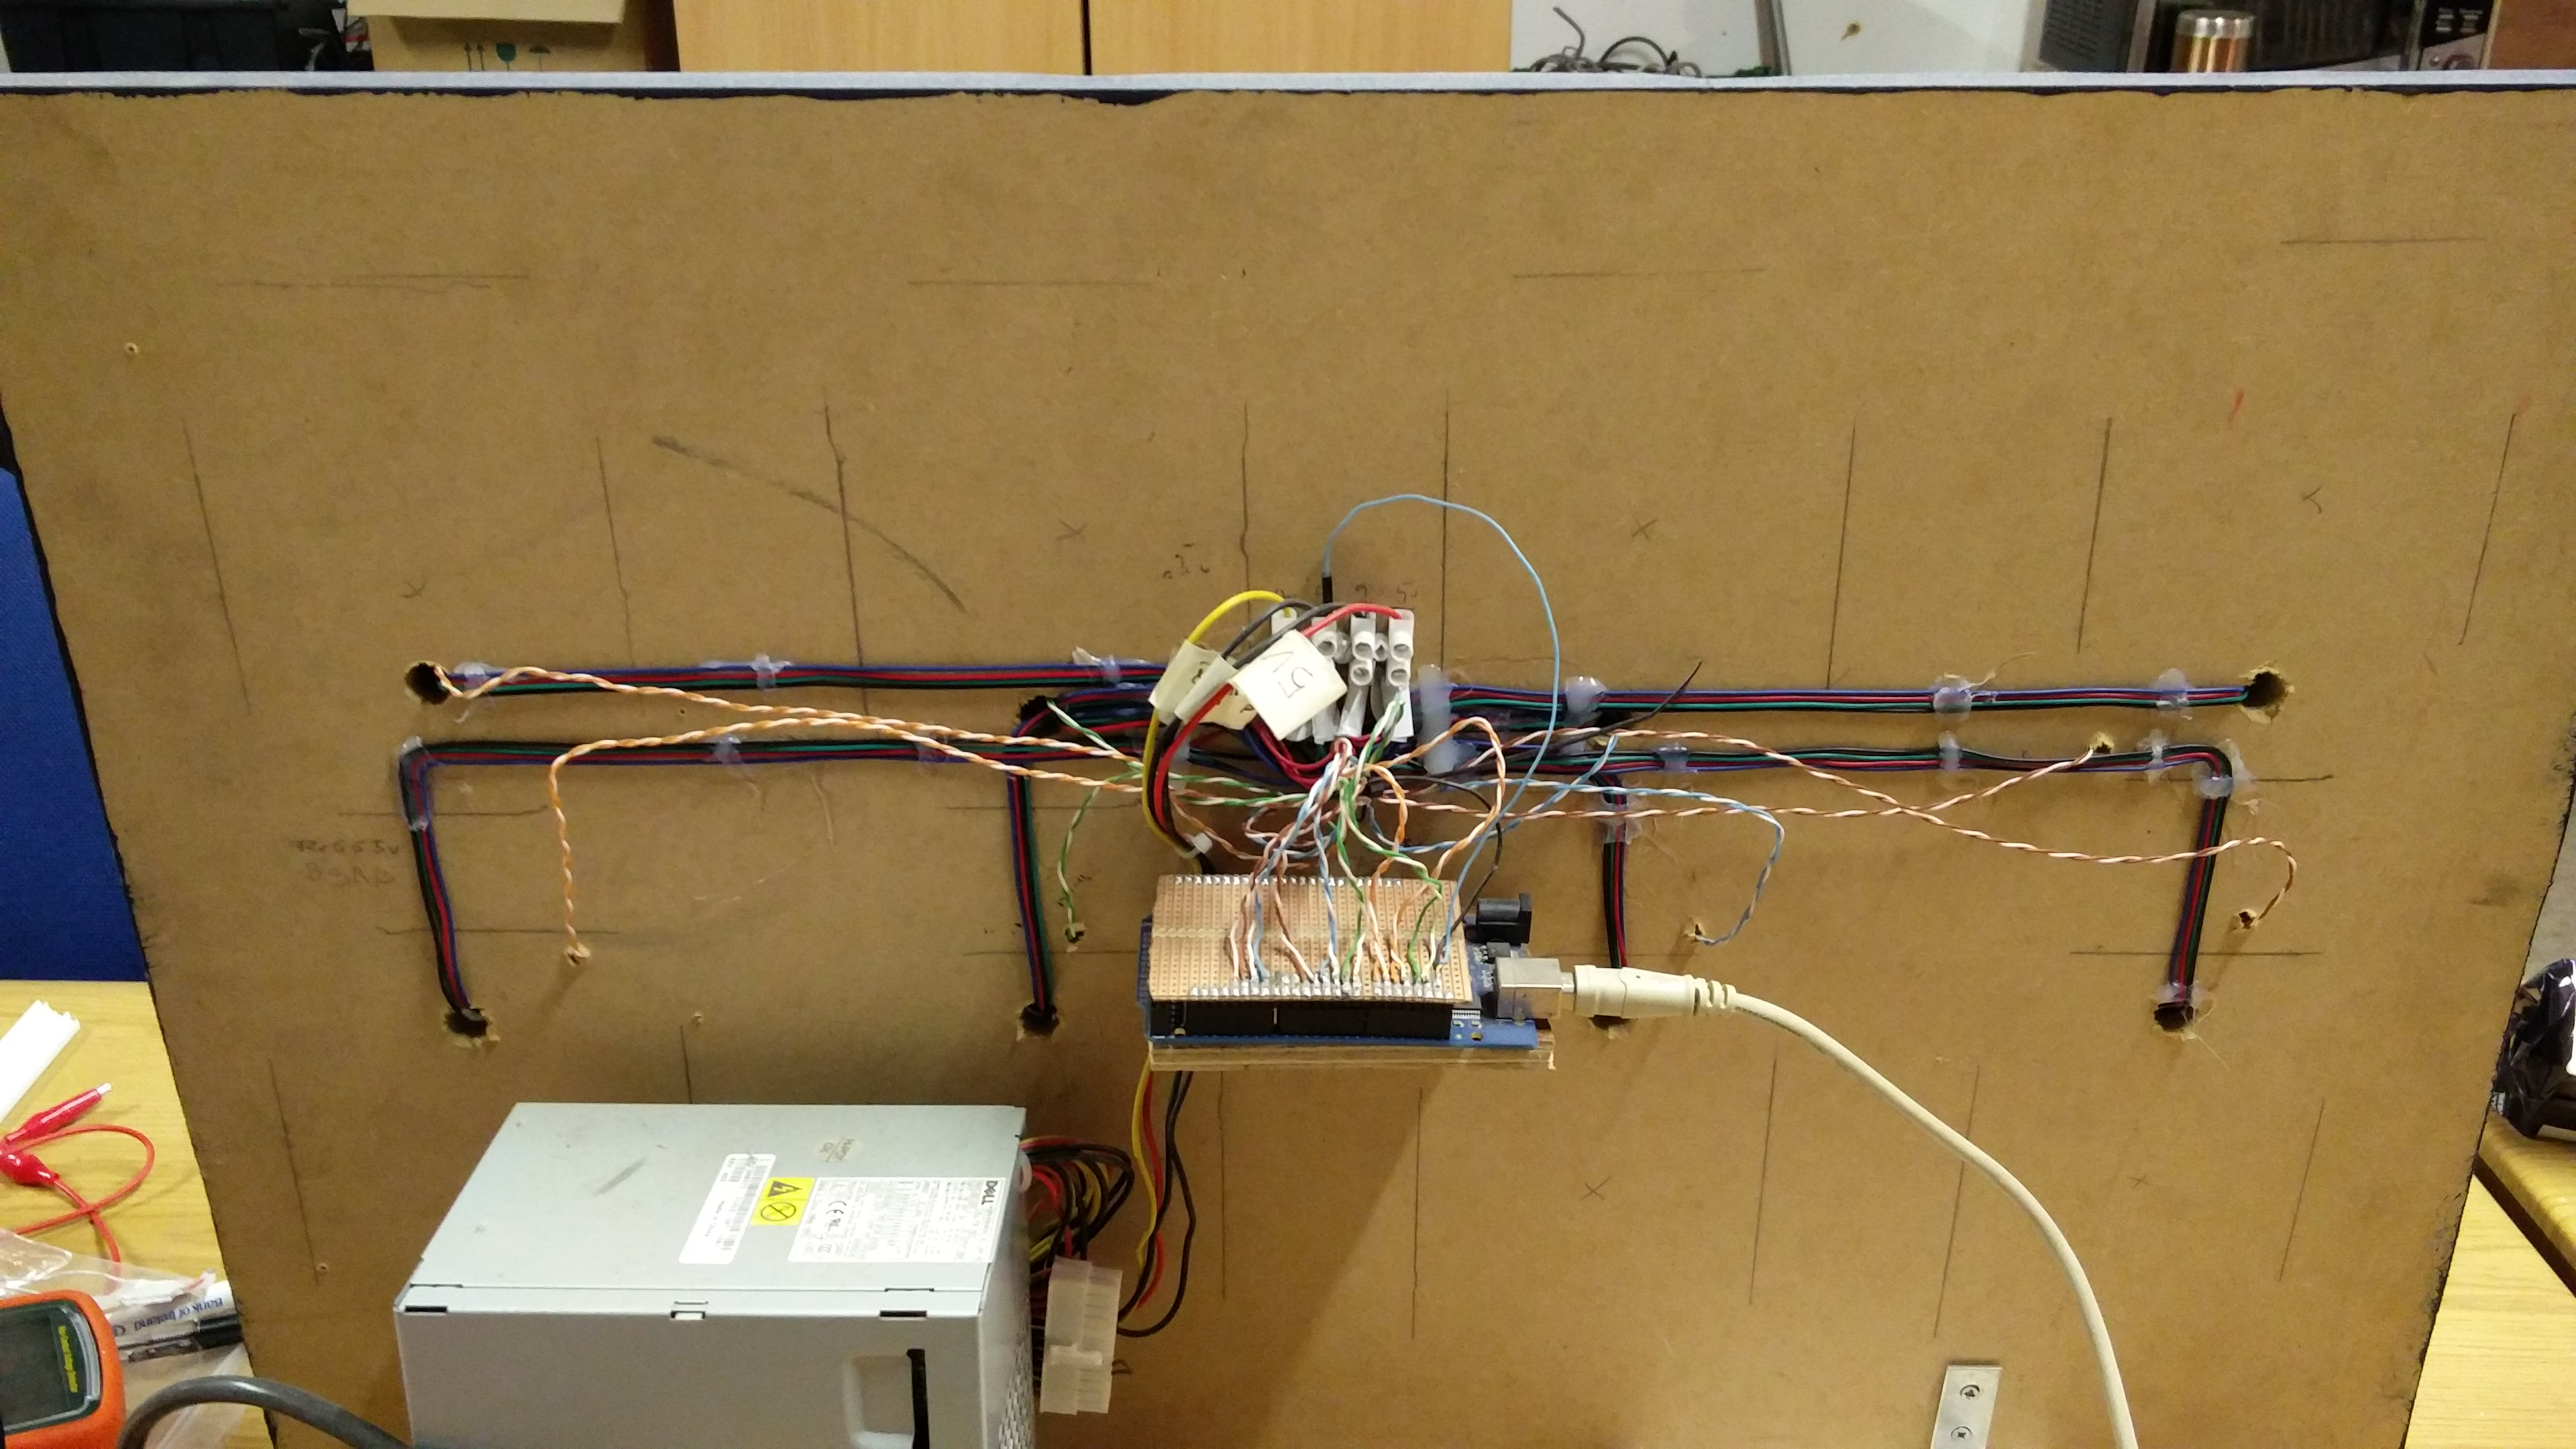
\includegraphics[width = 1.3in]{images/floppy_5}} &
			\subfloat{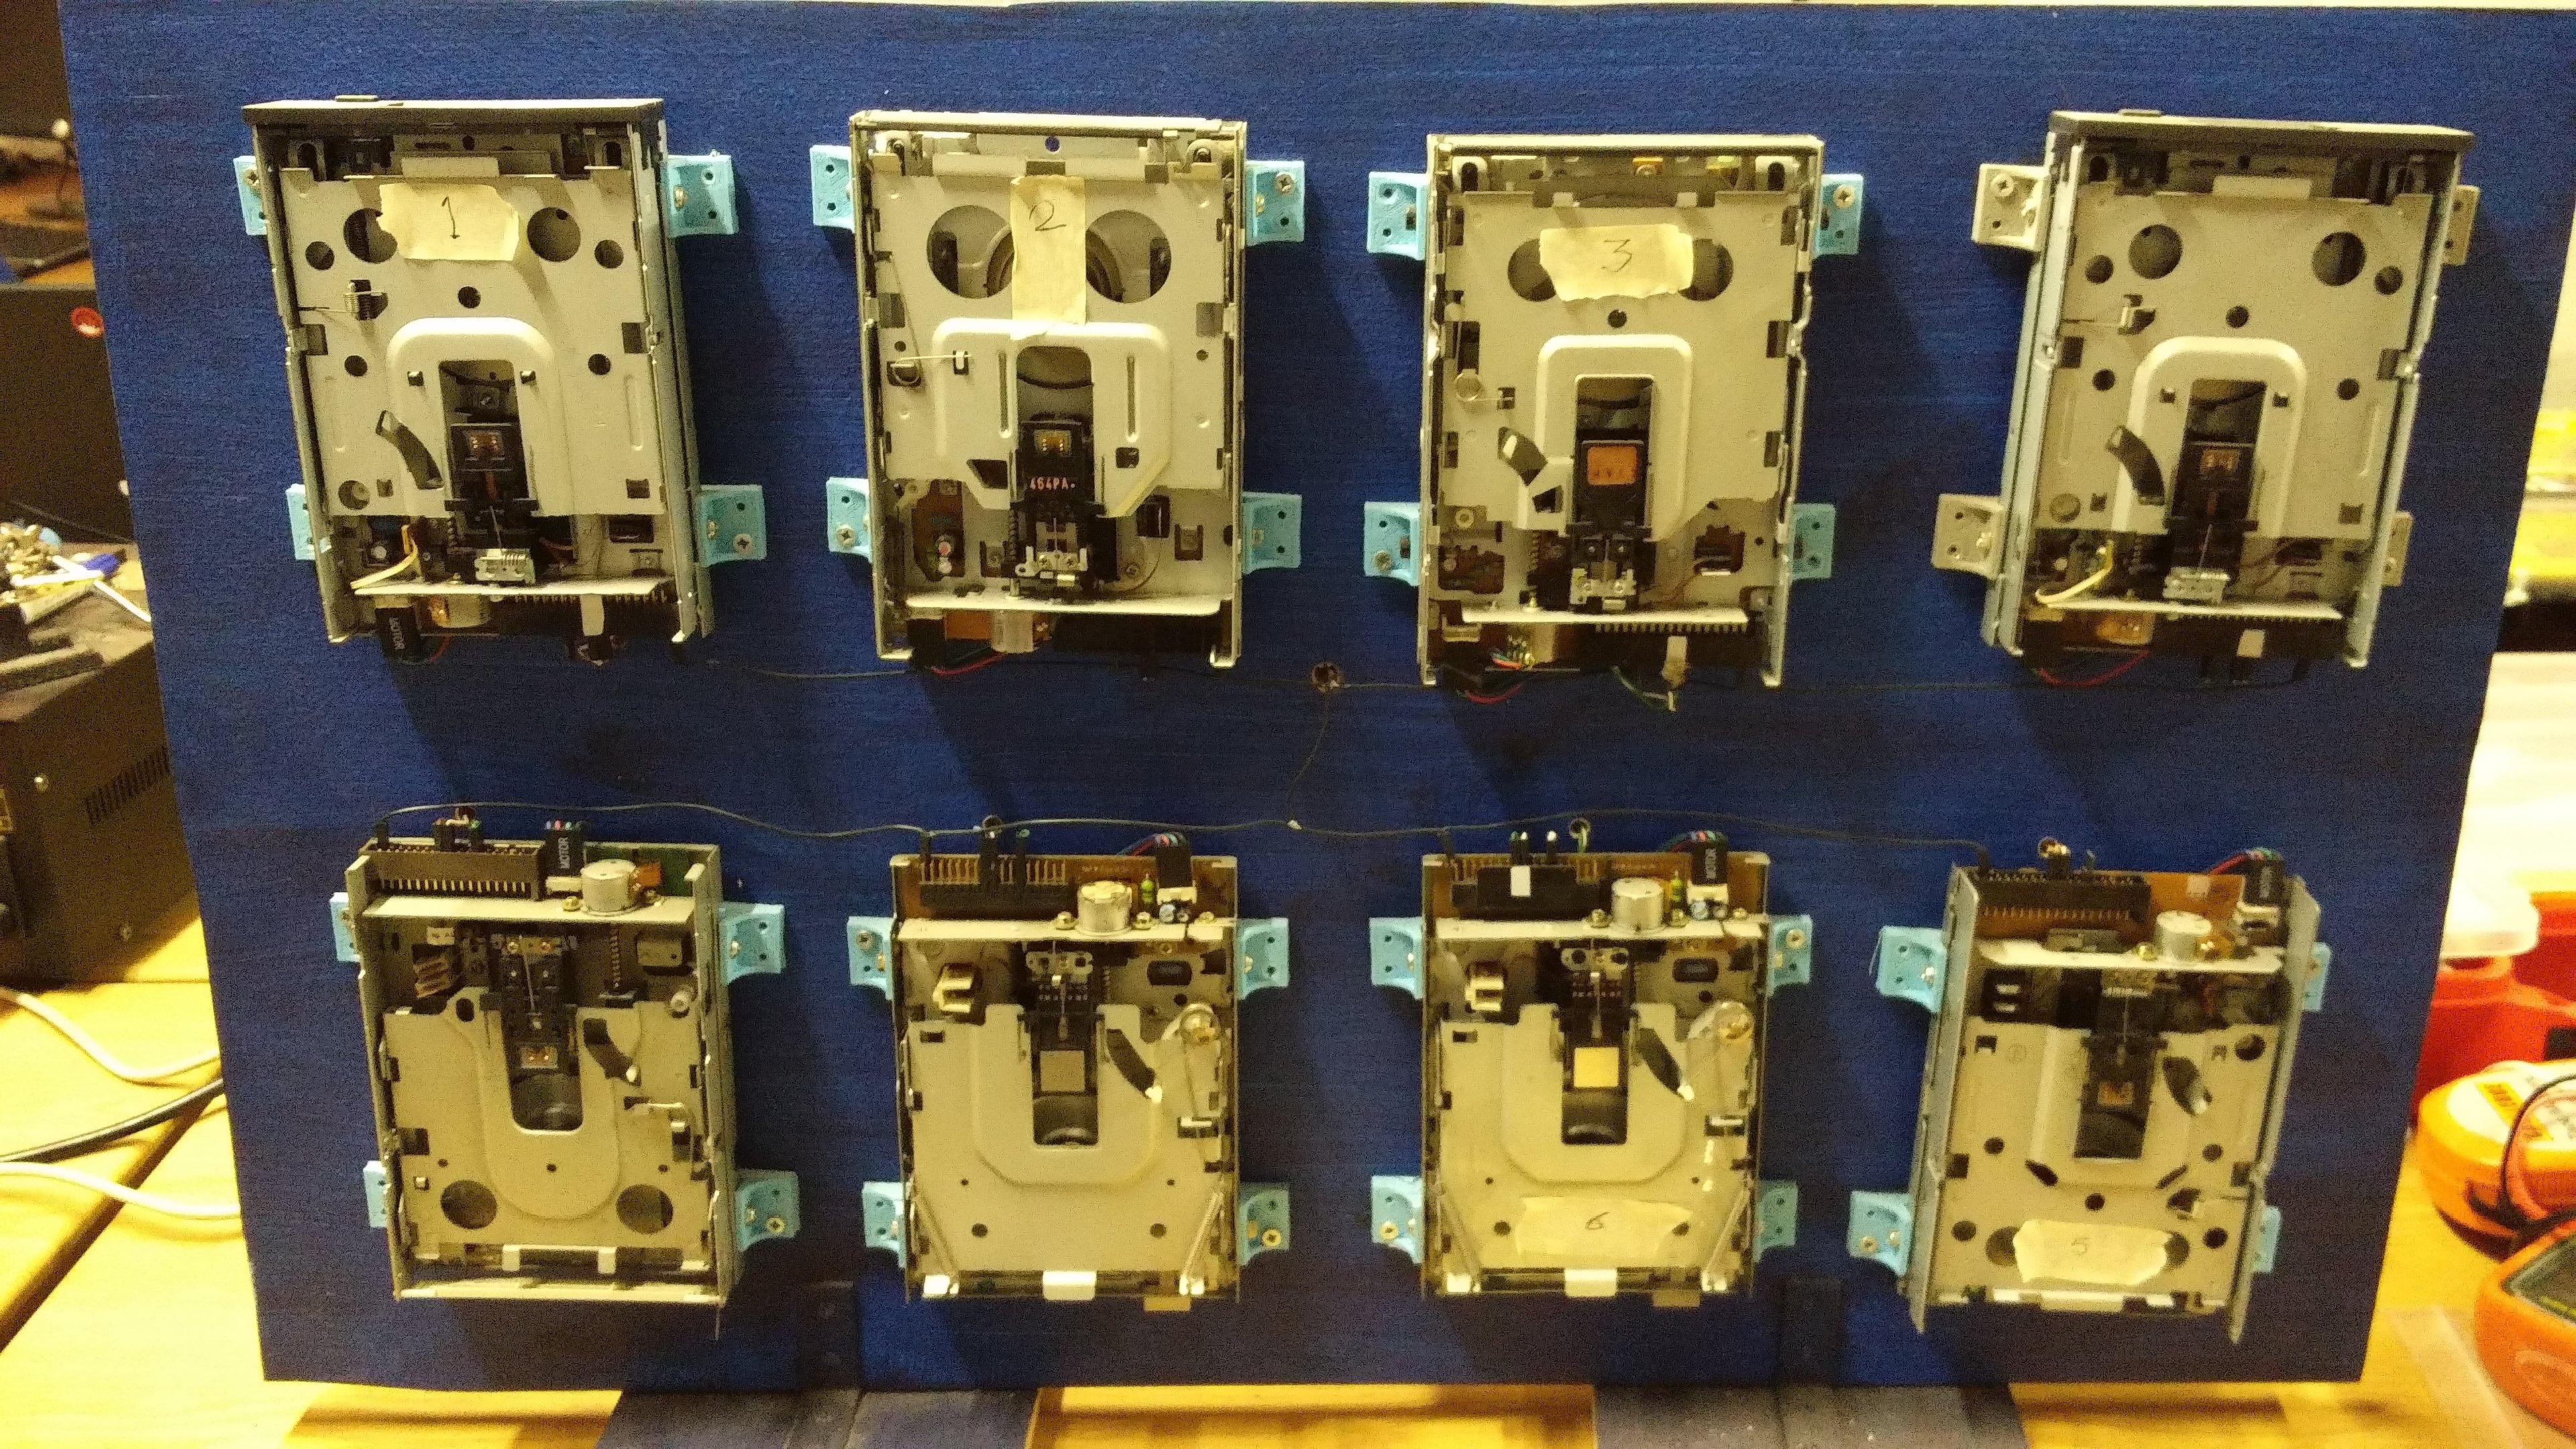
\includegraphics[width = 1.3in]{images/floppy_6}} 
		\end{tabular}
		\caption{Floppy Drive MIDI Player 2016}
	\end{figure}
\end{frame}


\section{Quadcopter Drone}
\begin{frame}{Quadcopter Drone}
	\begin{figure}
		\begin{tabular}{ccc}
			\subfloat{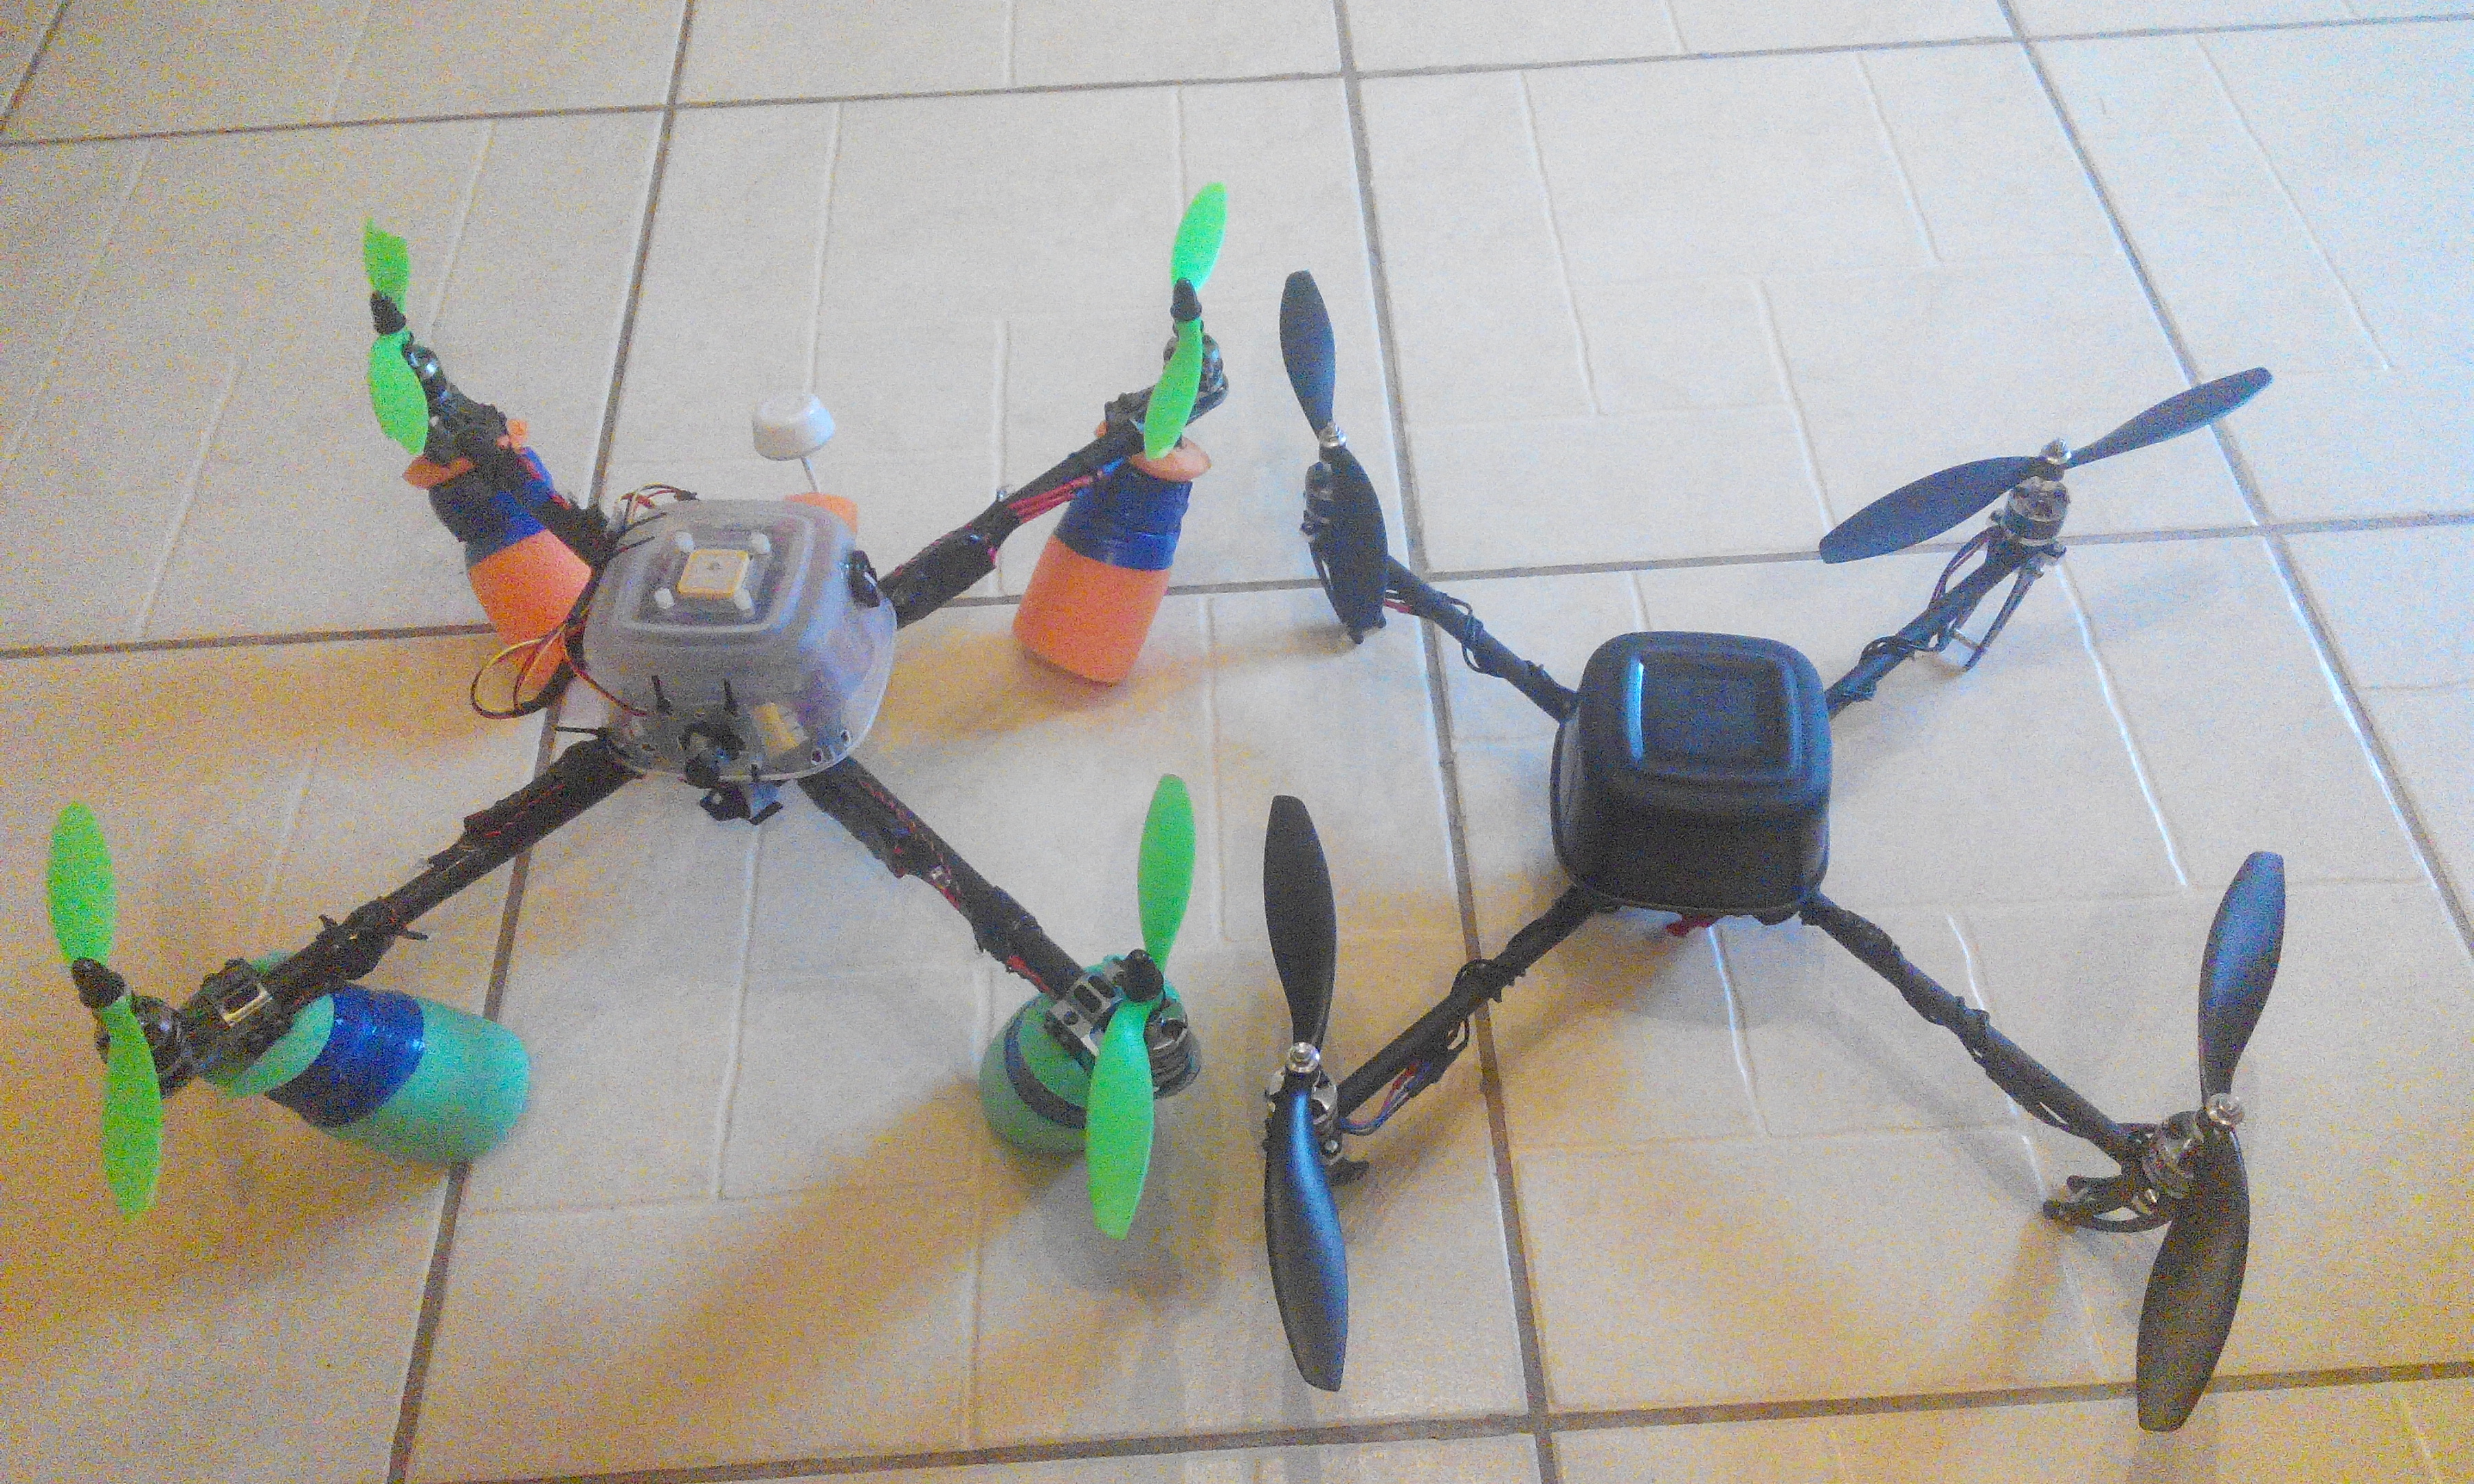
\includegraphics[width = 1.3in]{images/quad_1}} &
			\subfloat{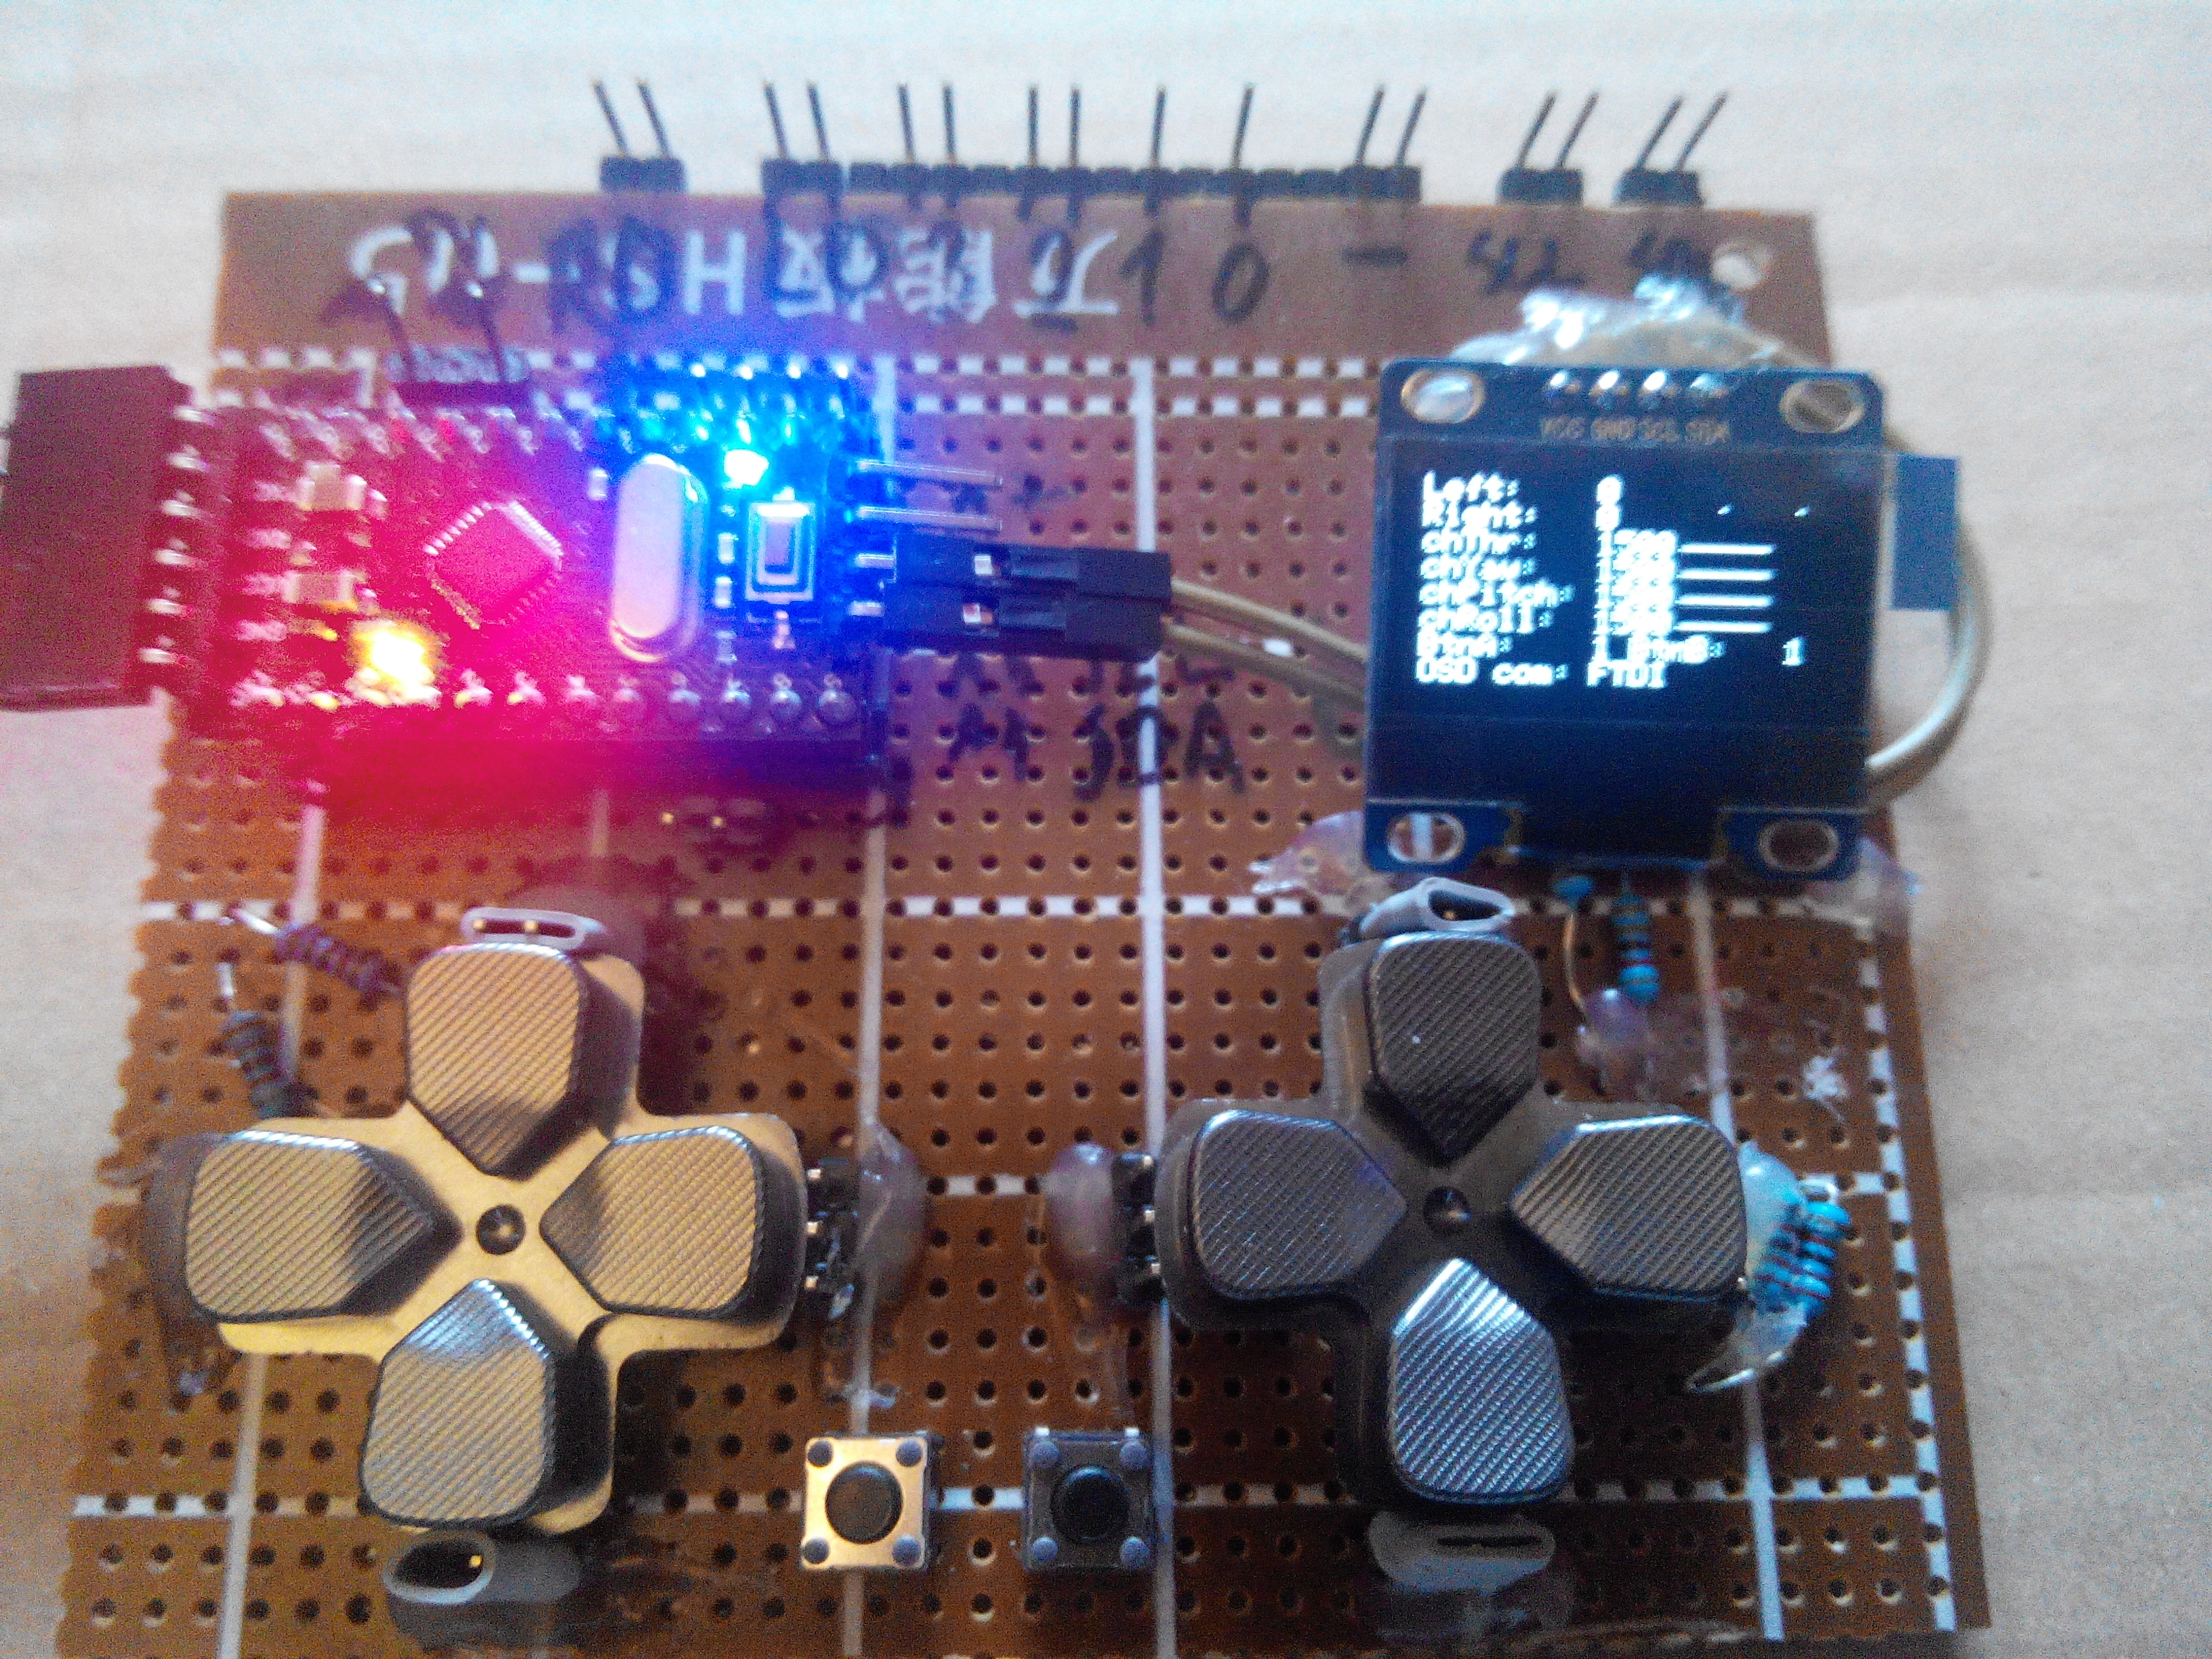
\includegraphics[width = 1.3in]{images/quad_2}} &
			\subfloat{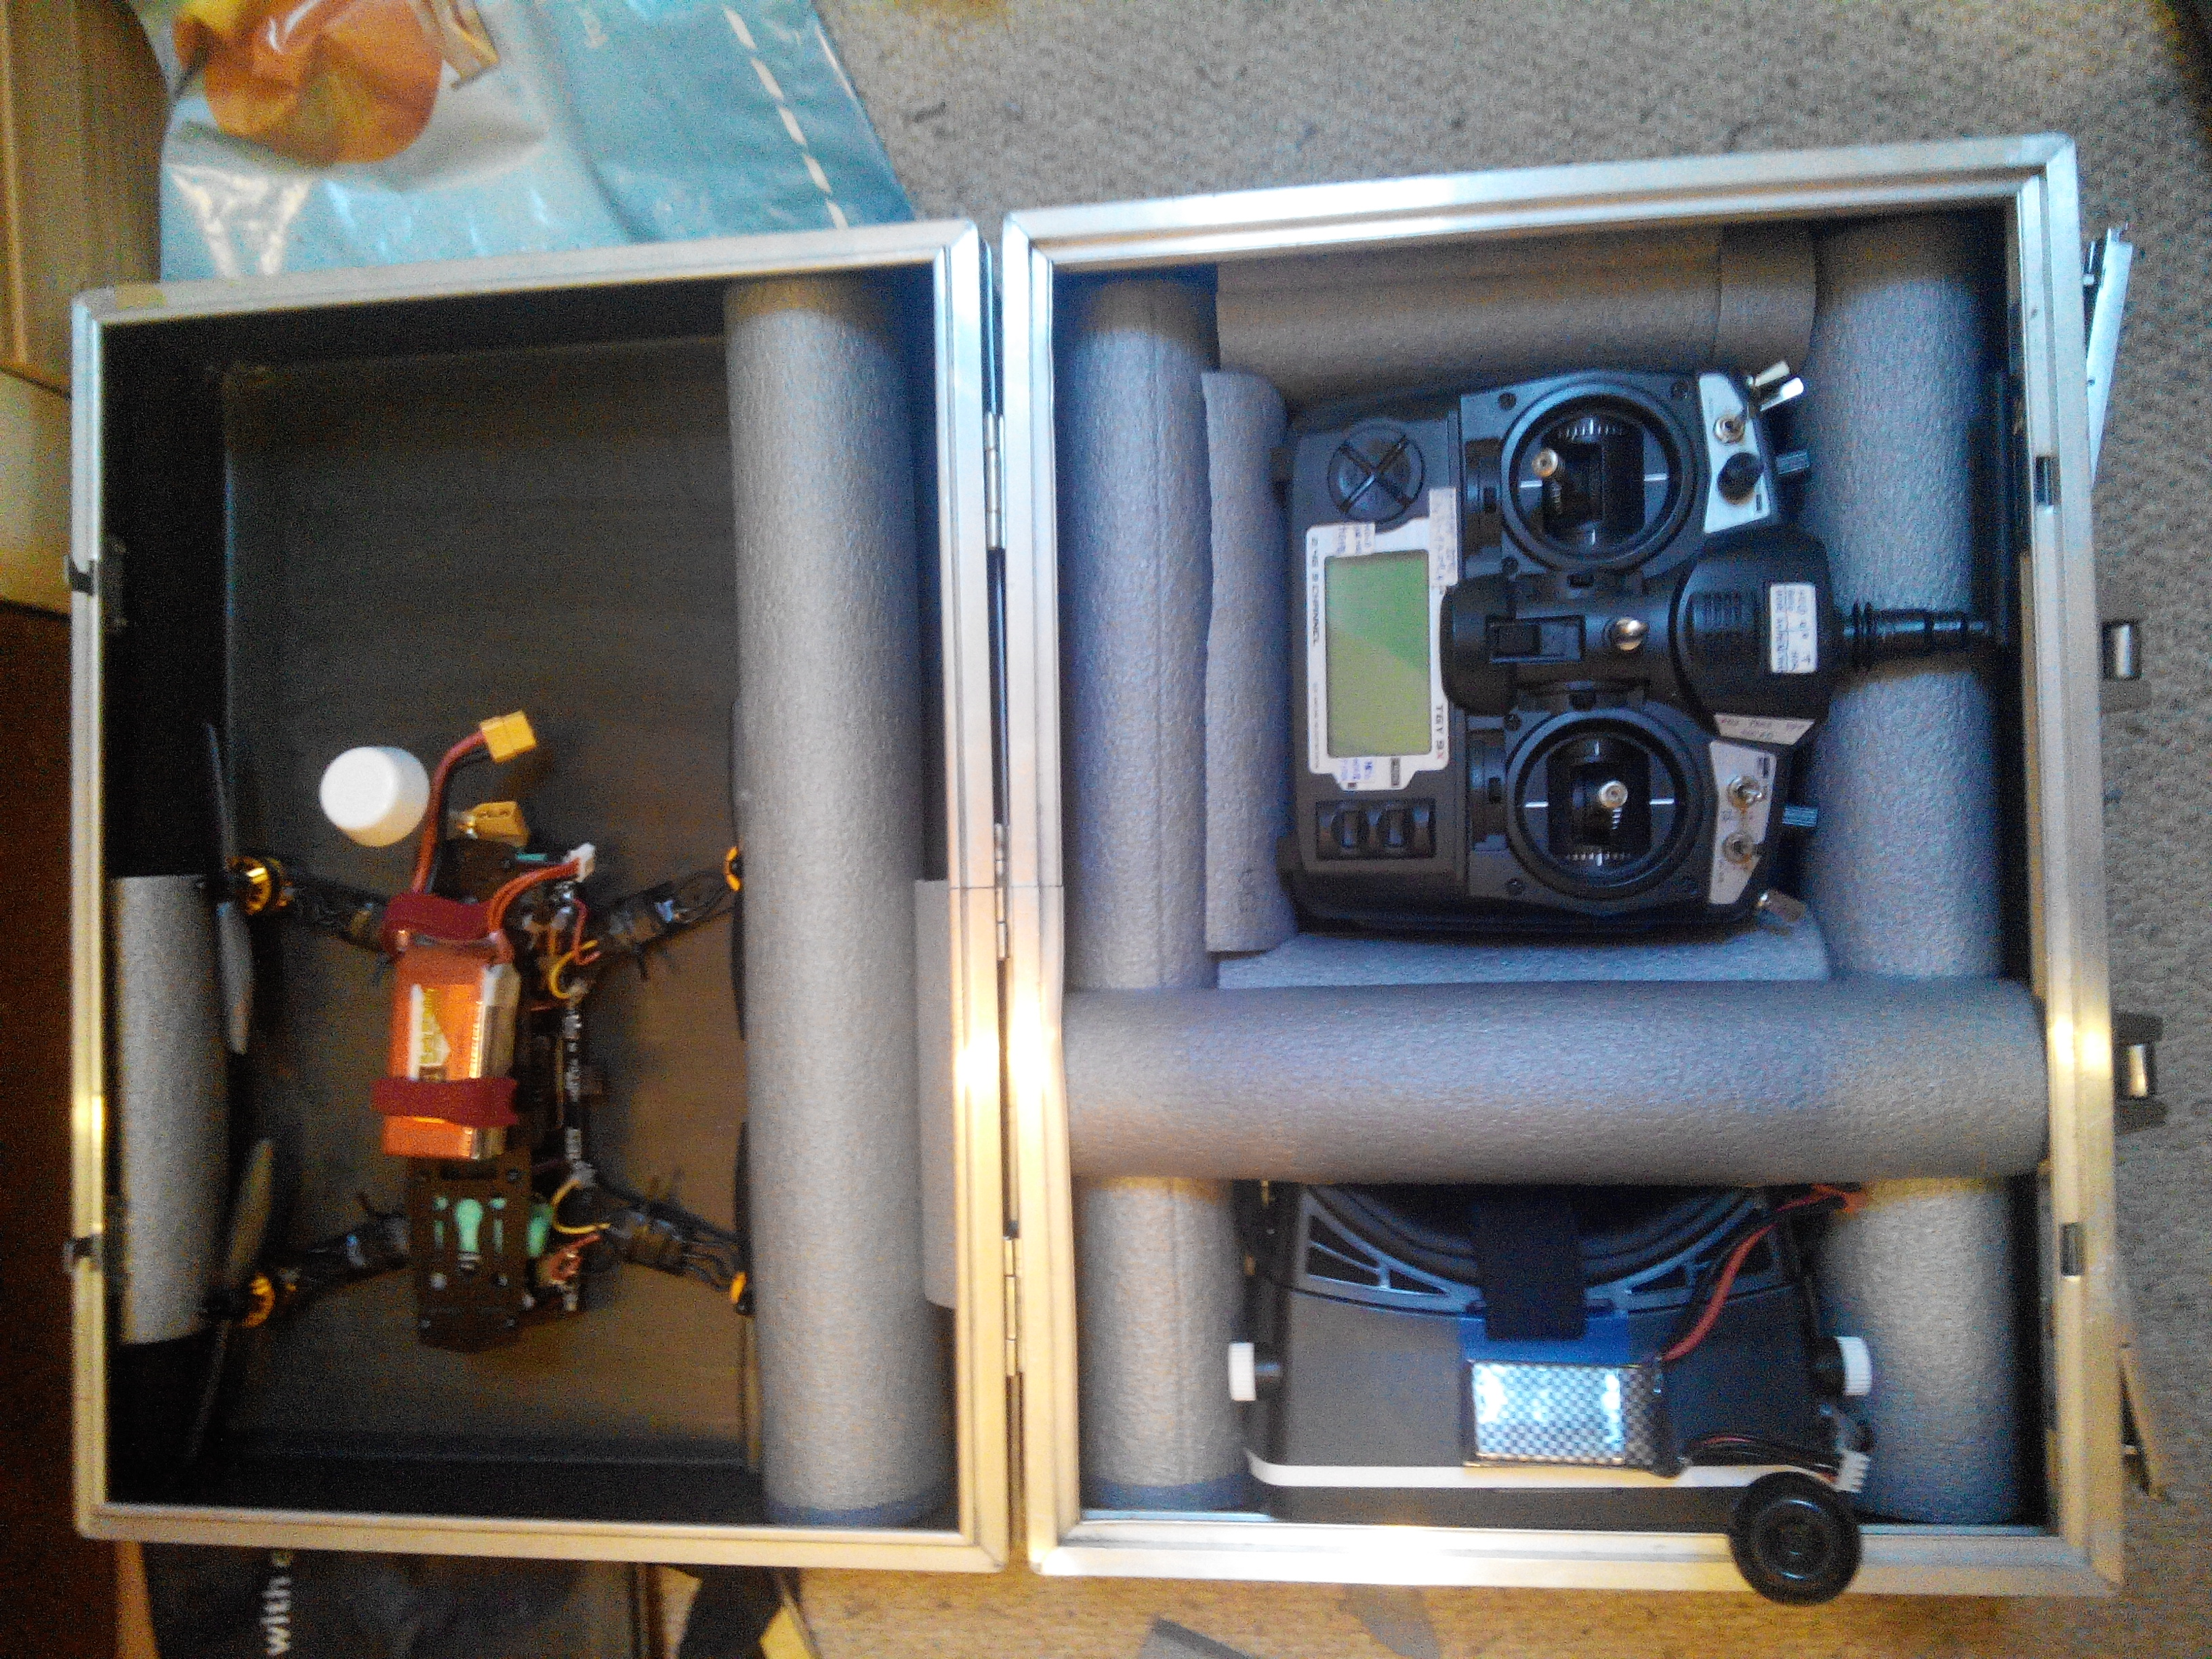
\includegraphics[width = 1.3in]{images/quad_3}}
		\end{tabular}
		\caption{Quadcopter Drone 2015/2016}
	\end{figure}
\end{frame}


\section{3D Printer}
\begin{frame}{3D Printer}
\begin{figure}
	\begin{tabular}{ccc}
		\subfloat{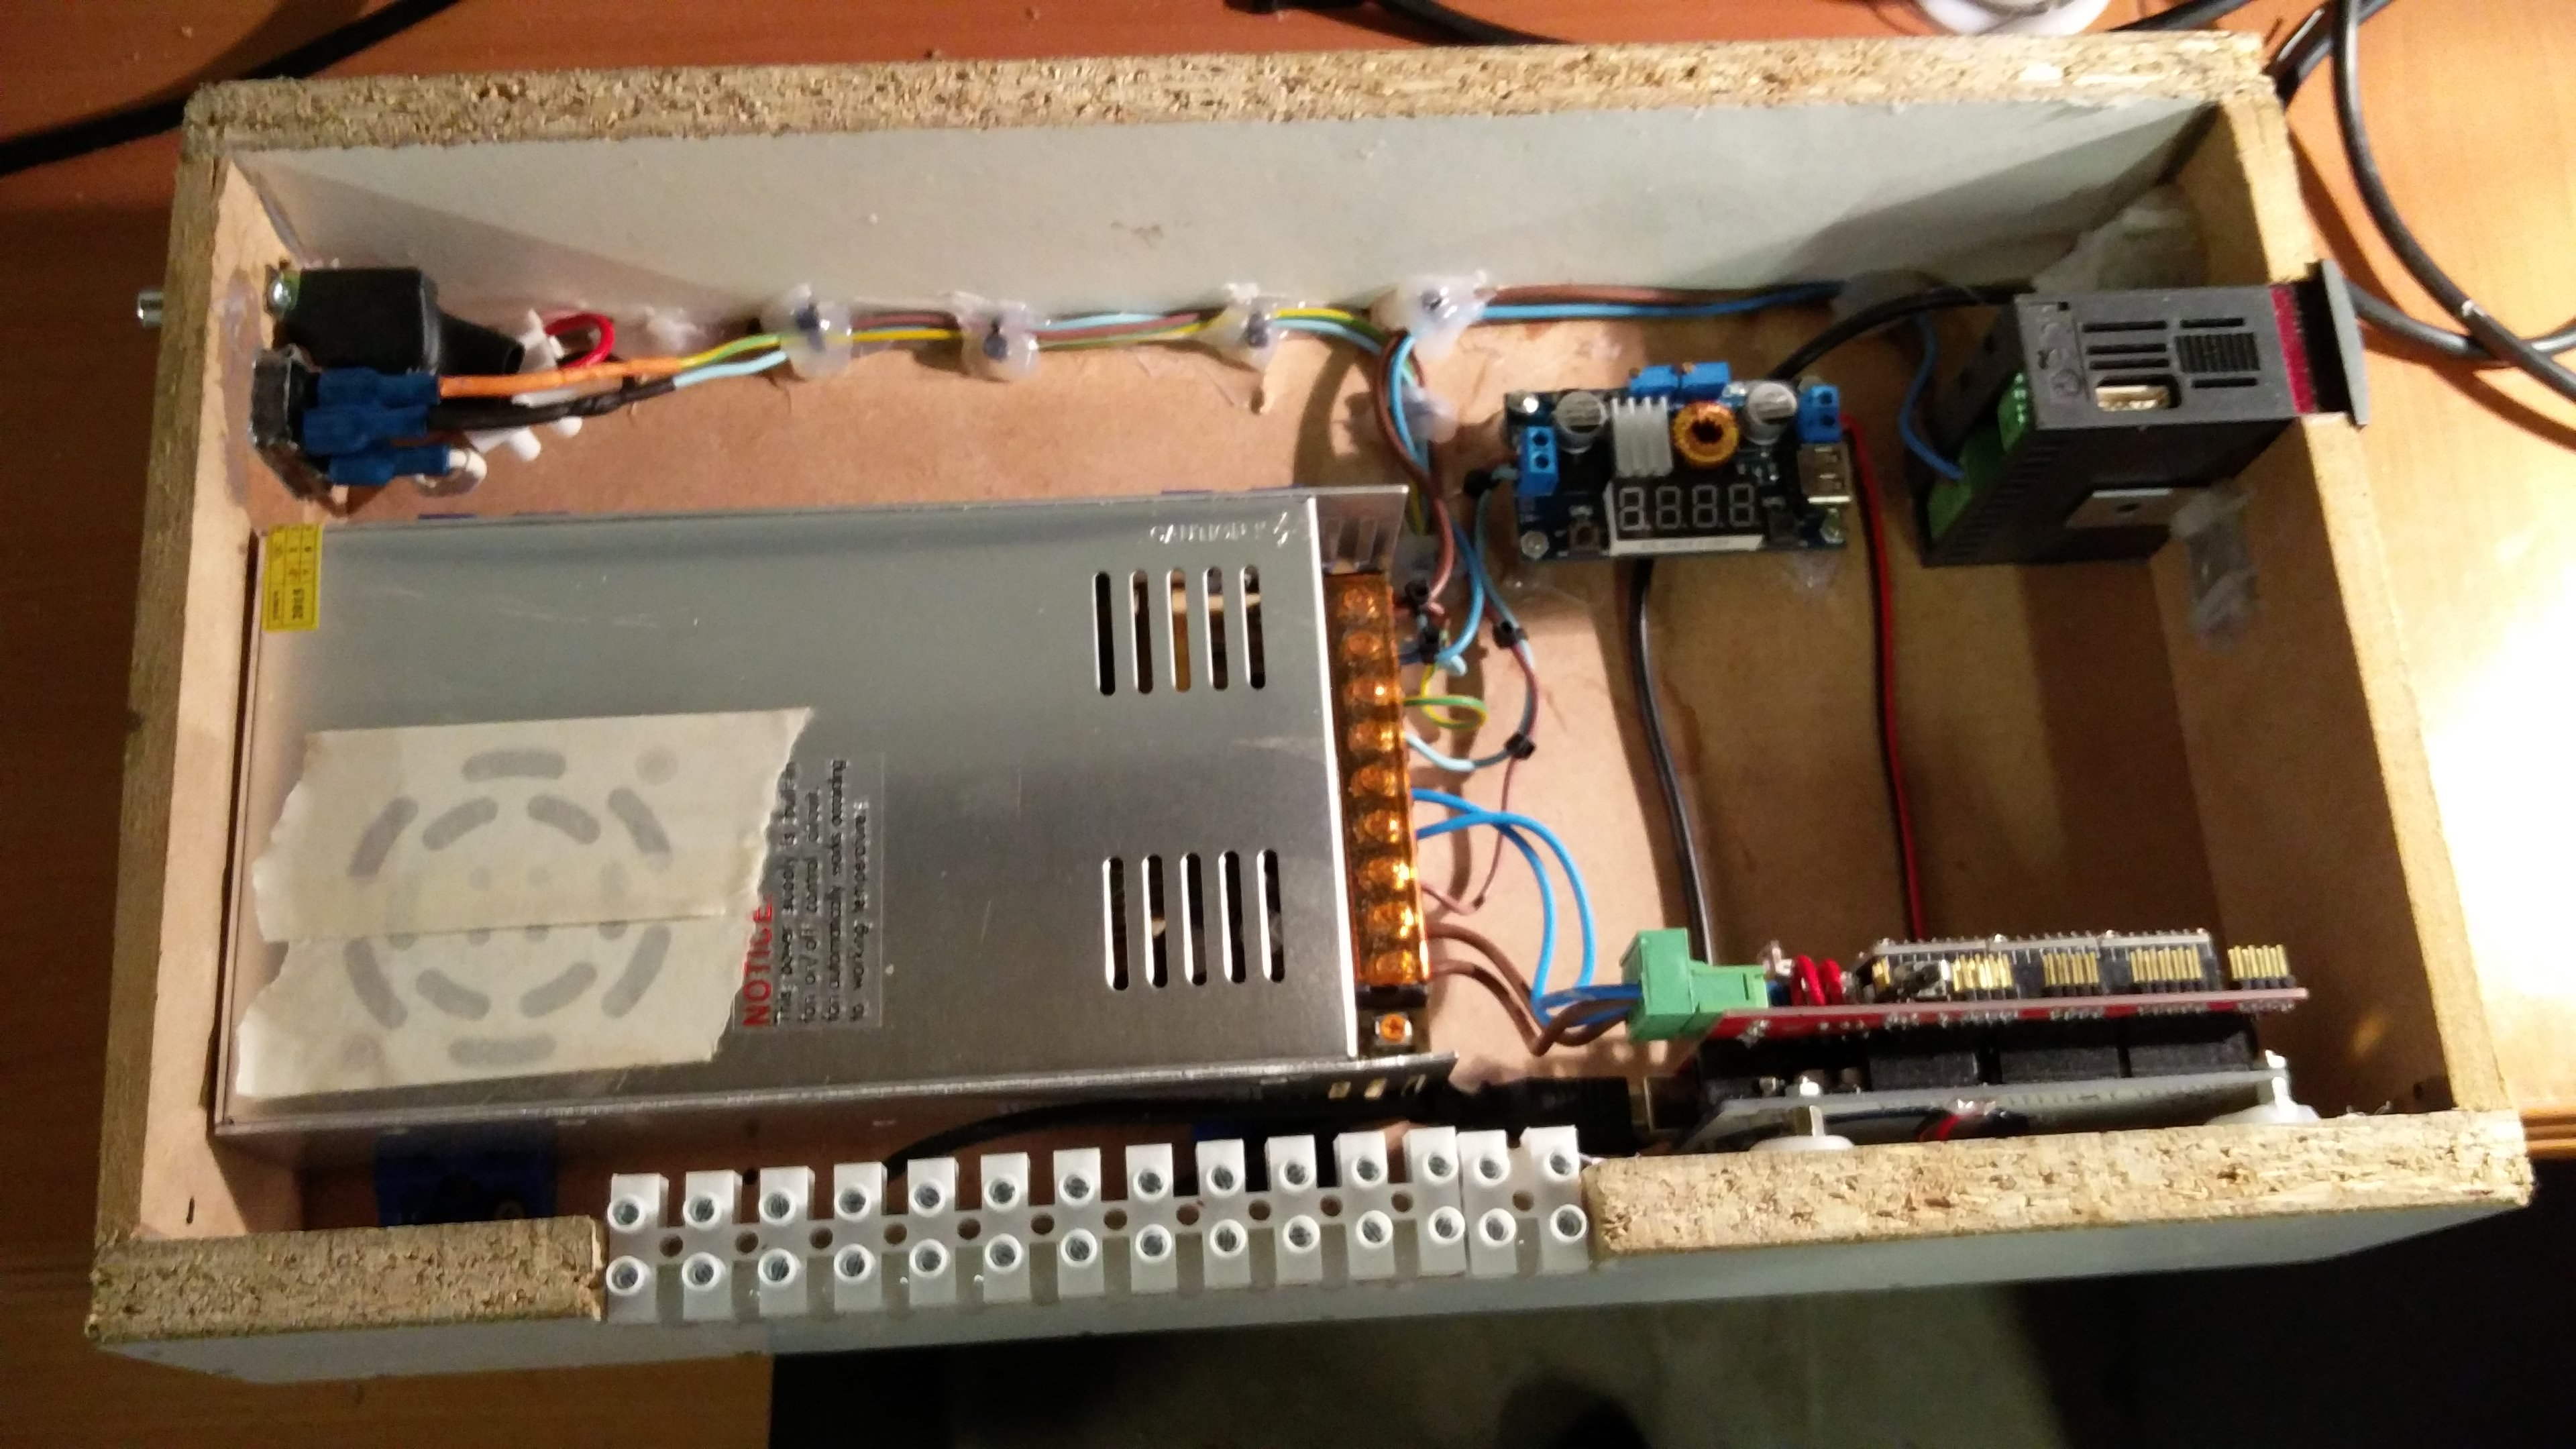
\includegraphics[width = 1.3in]{images/3dprinter_1}} &
		\subfloat{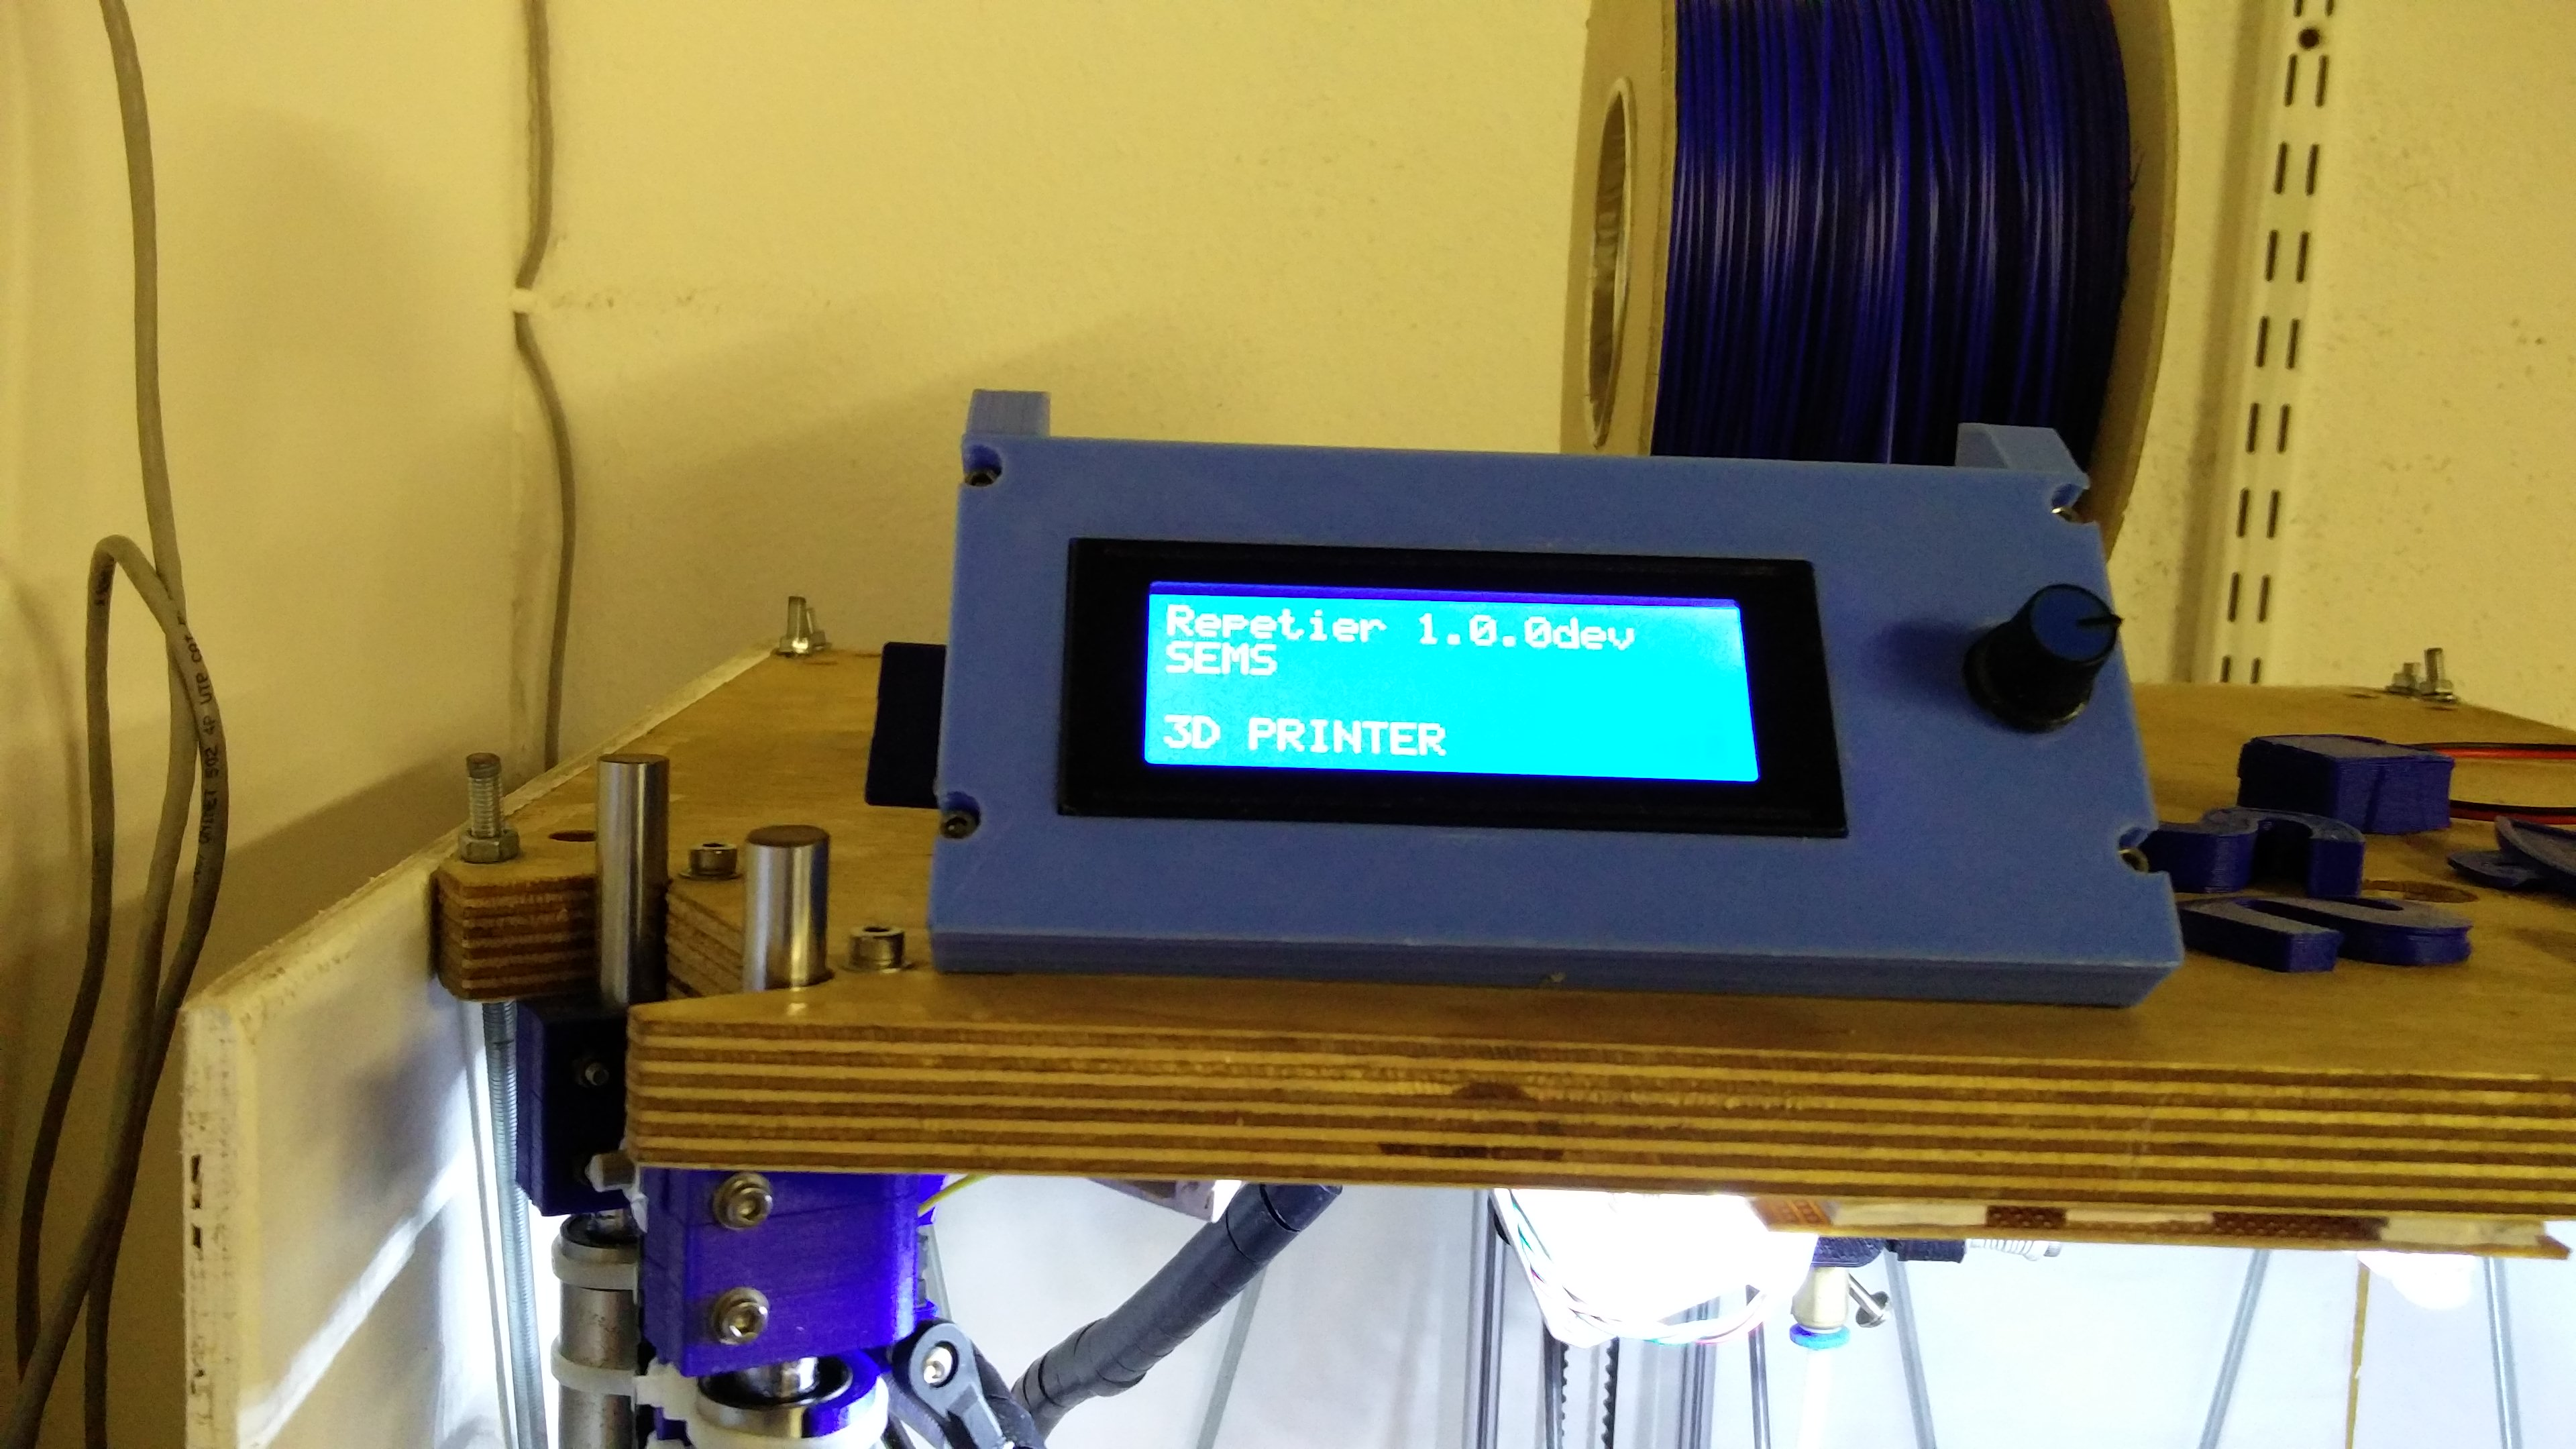
\includegraphics[width = 1.3in]{images/3dprinter_2}} &
		\subfloat{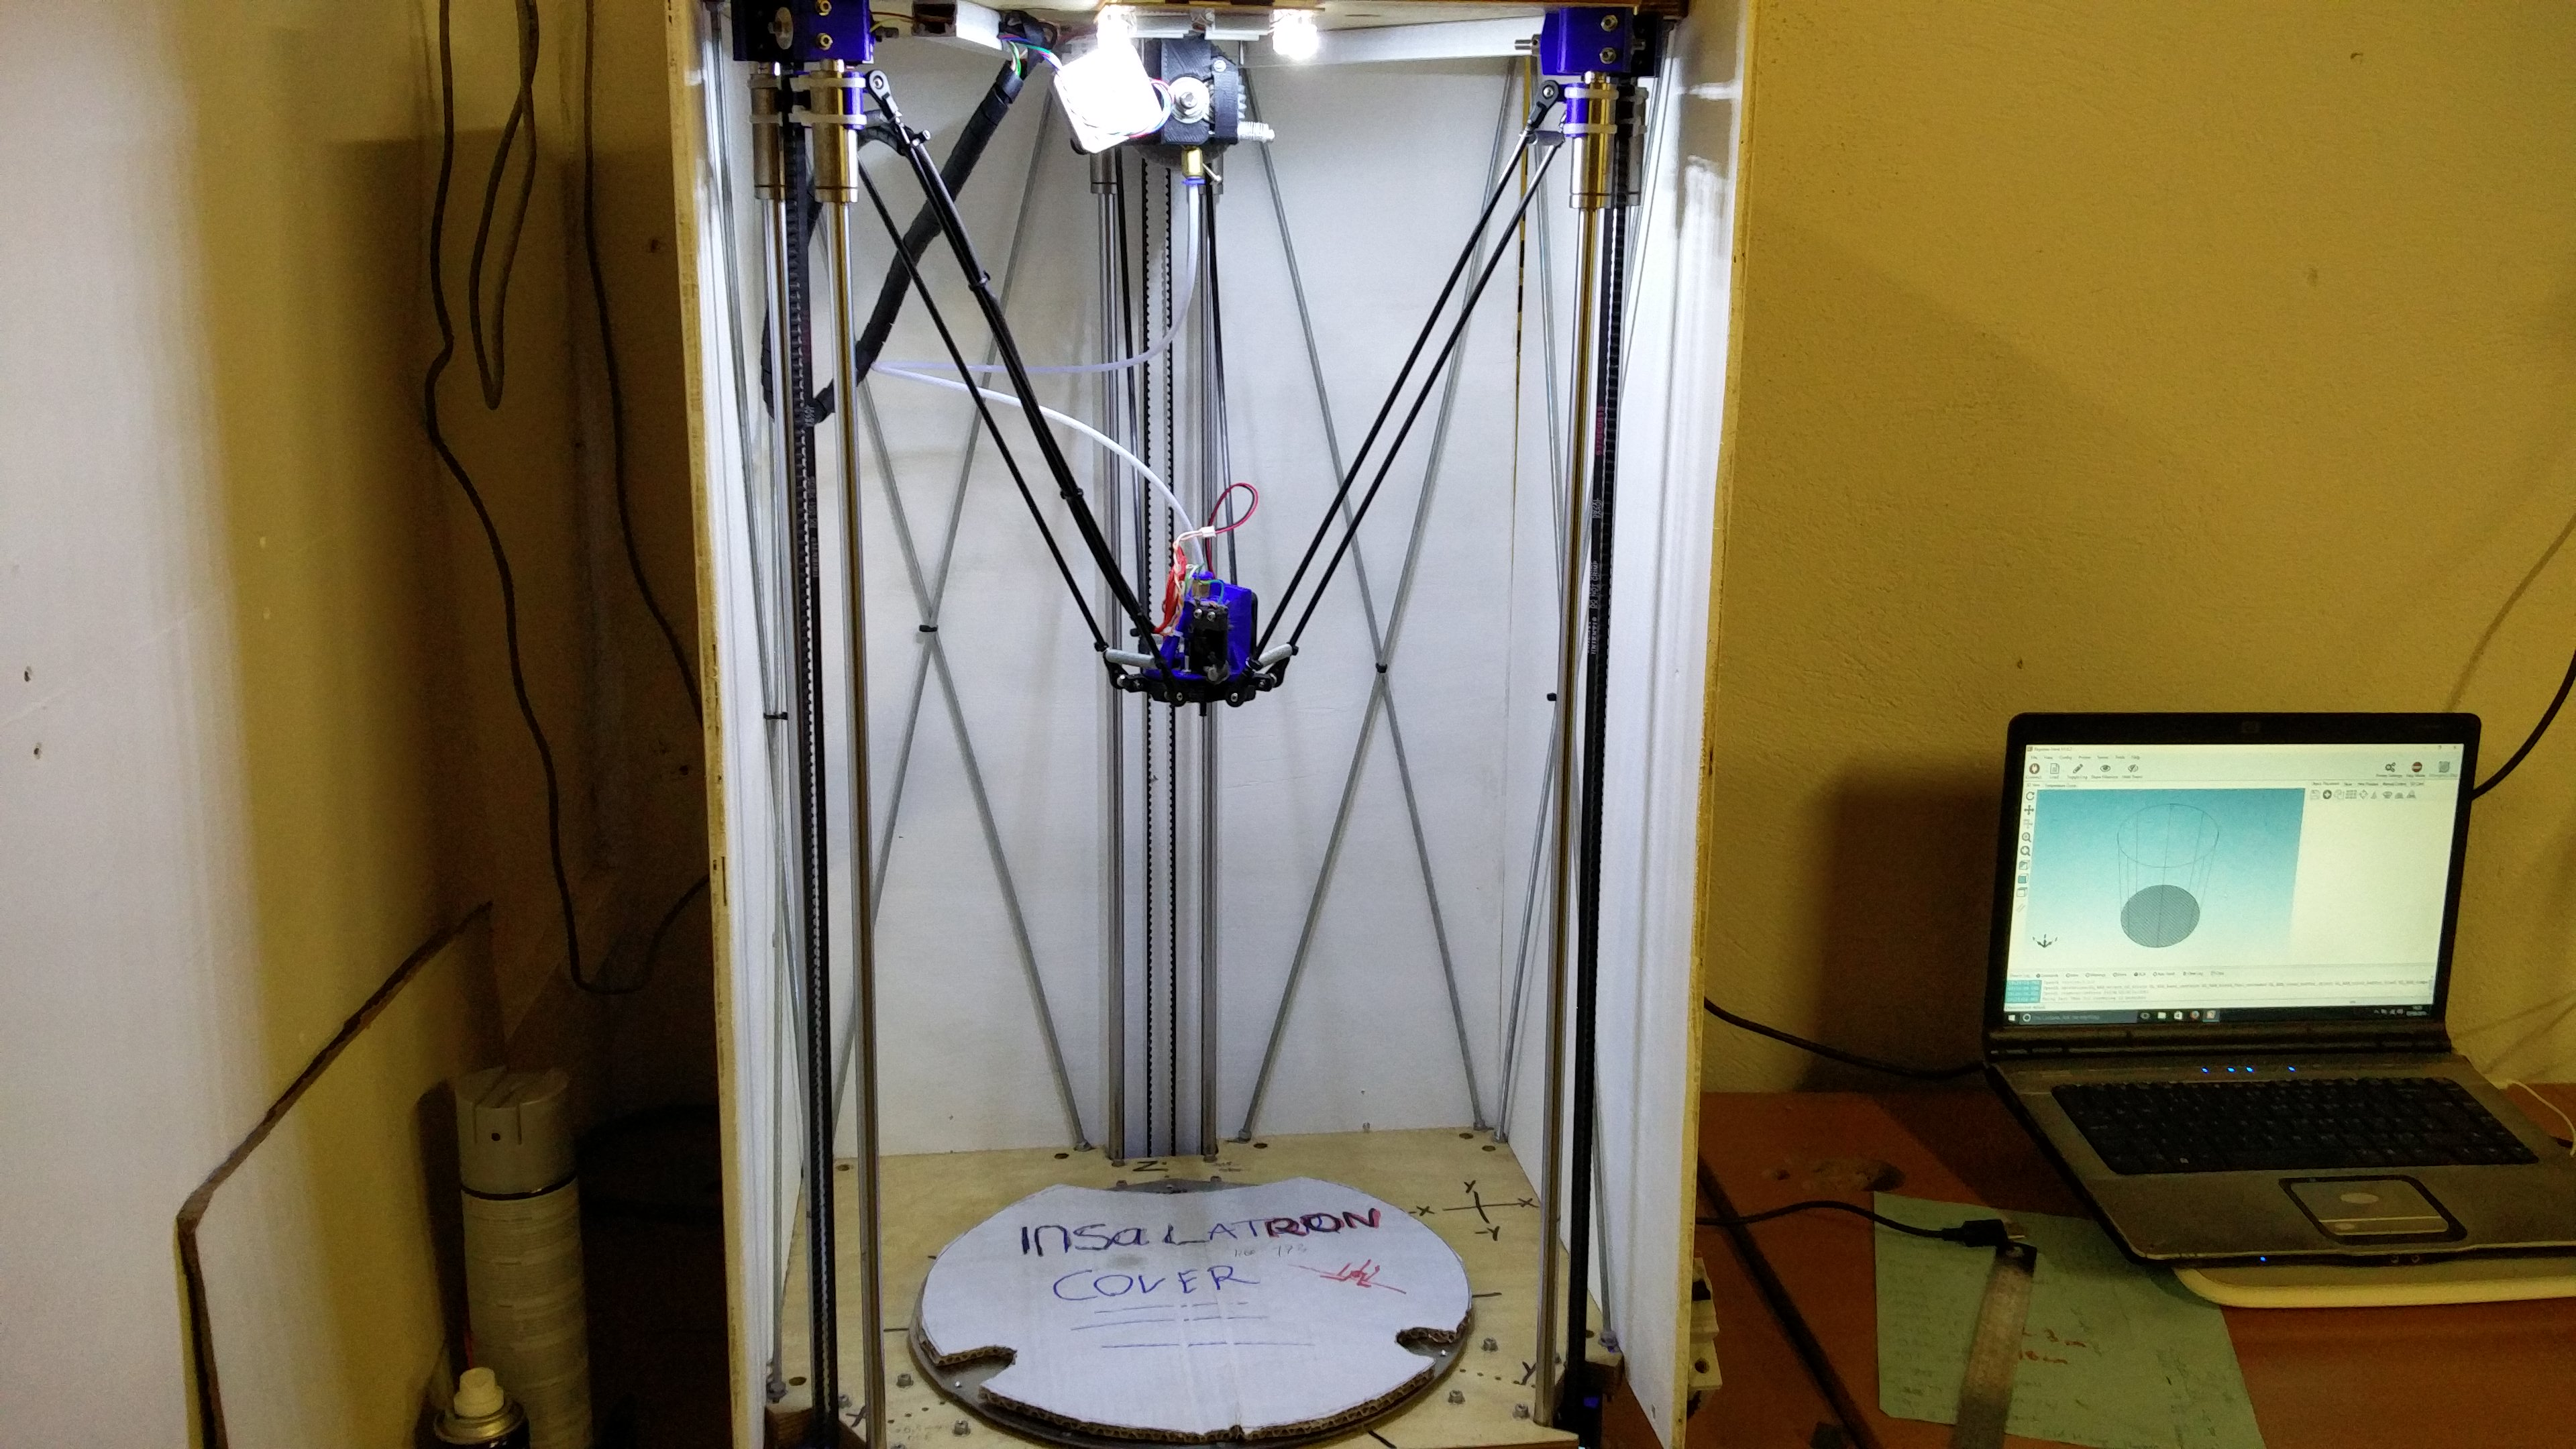
\includegraphics[width = 1.3in]{images/3dprinter_3}} \\
		\subfloat{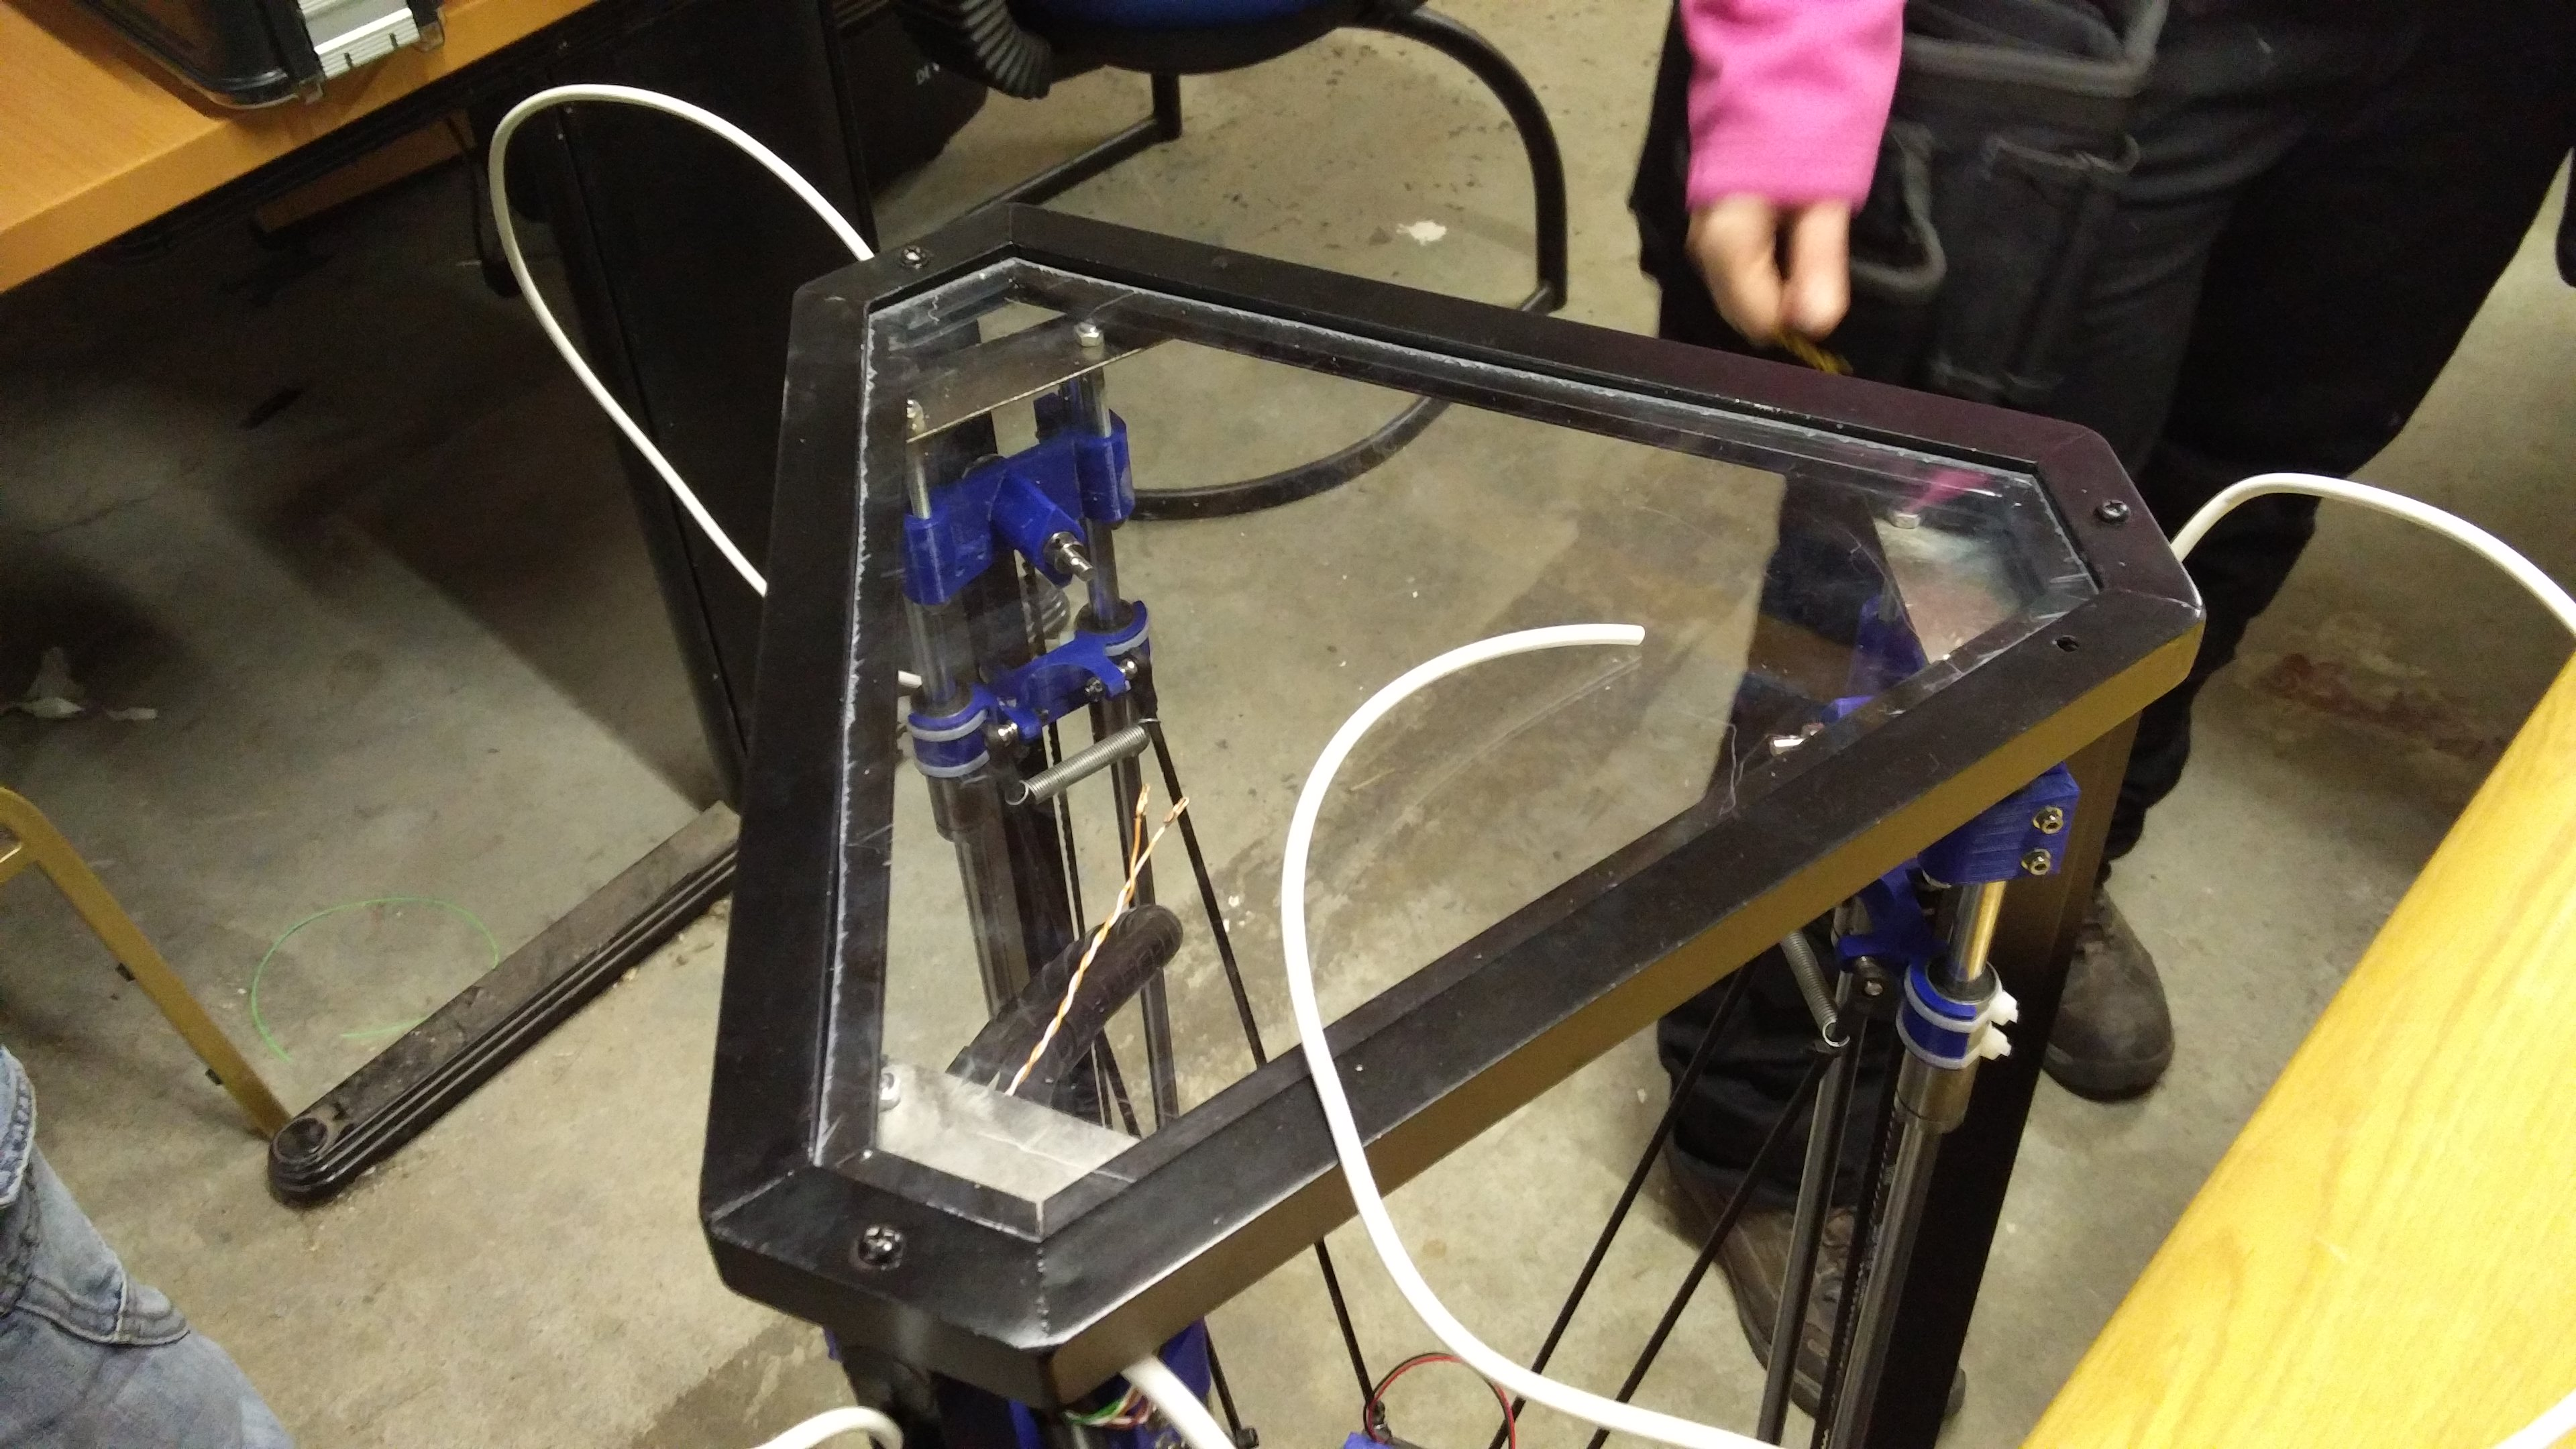
\includegraphics[width = 1.3in]{images/3dprinter_4}} &    \subfloat{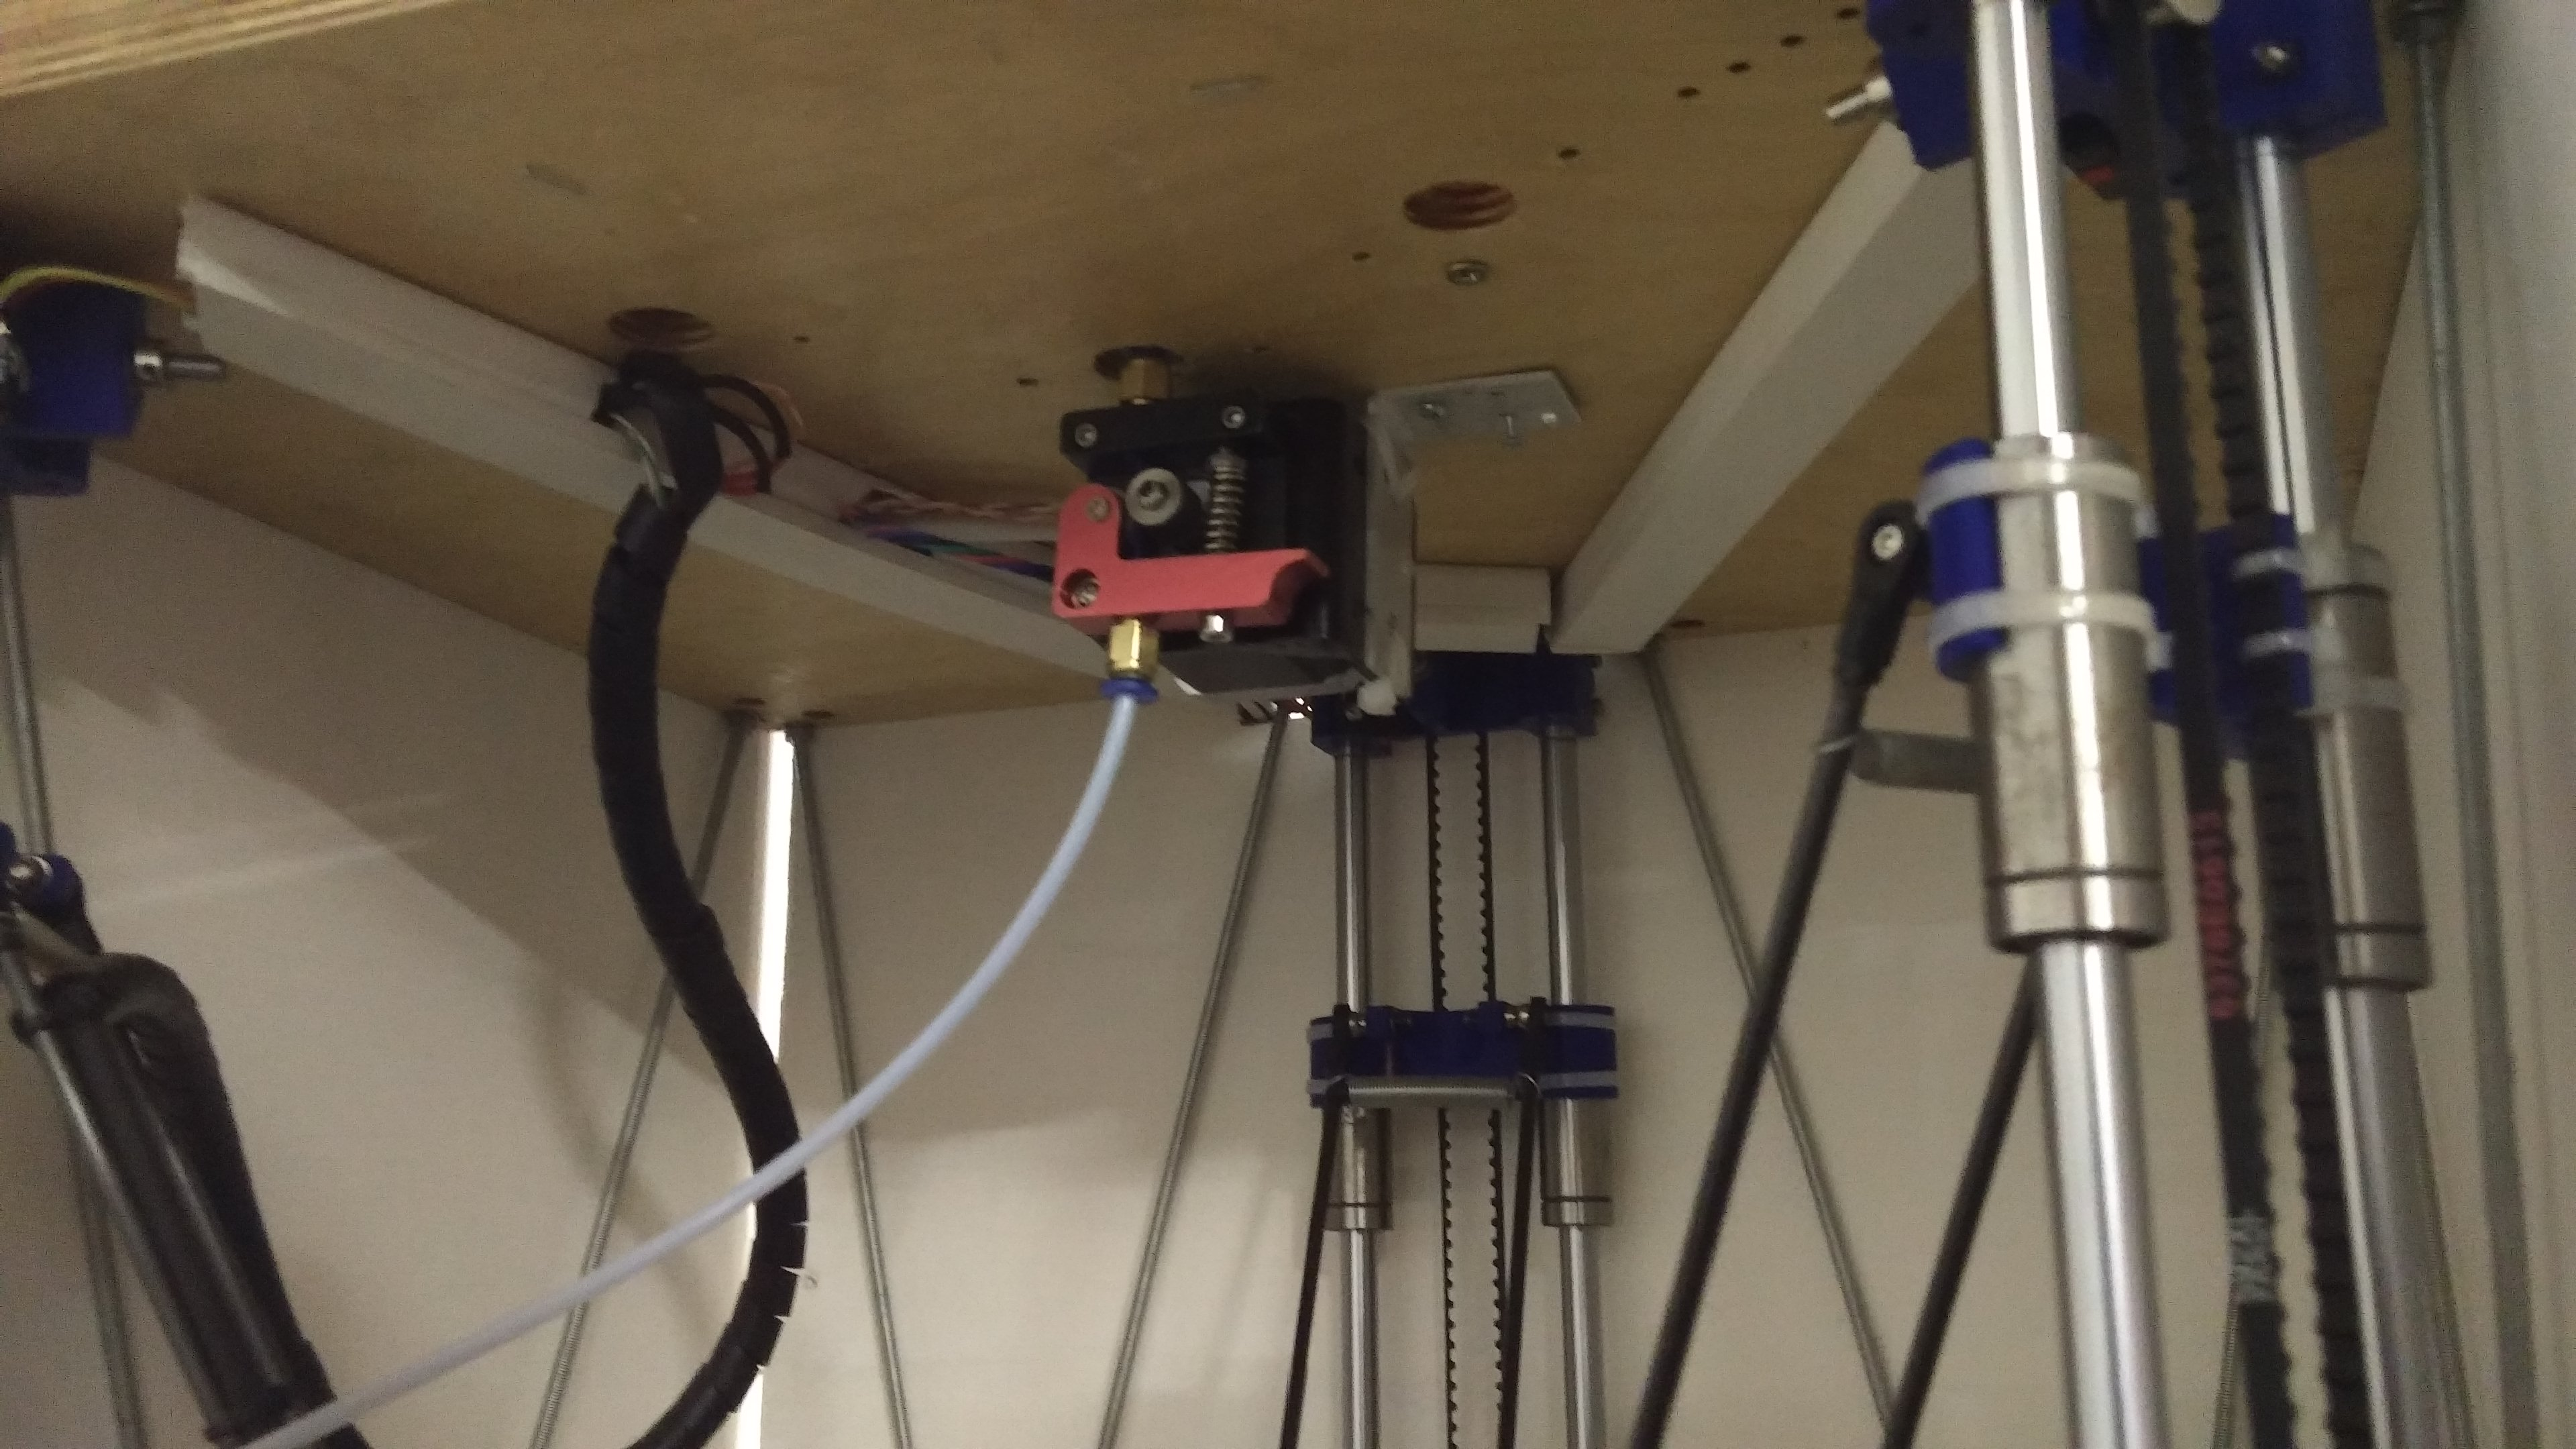
\includegraphics[width = 1.3in]{images/3dprinter_5}} &
		\subfloat{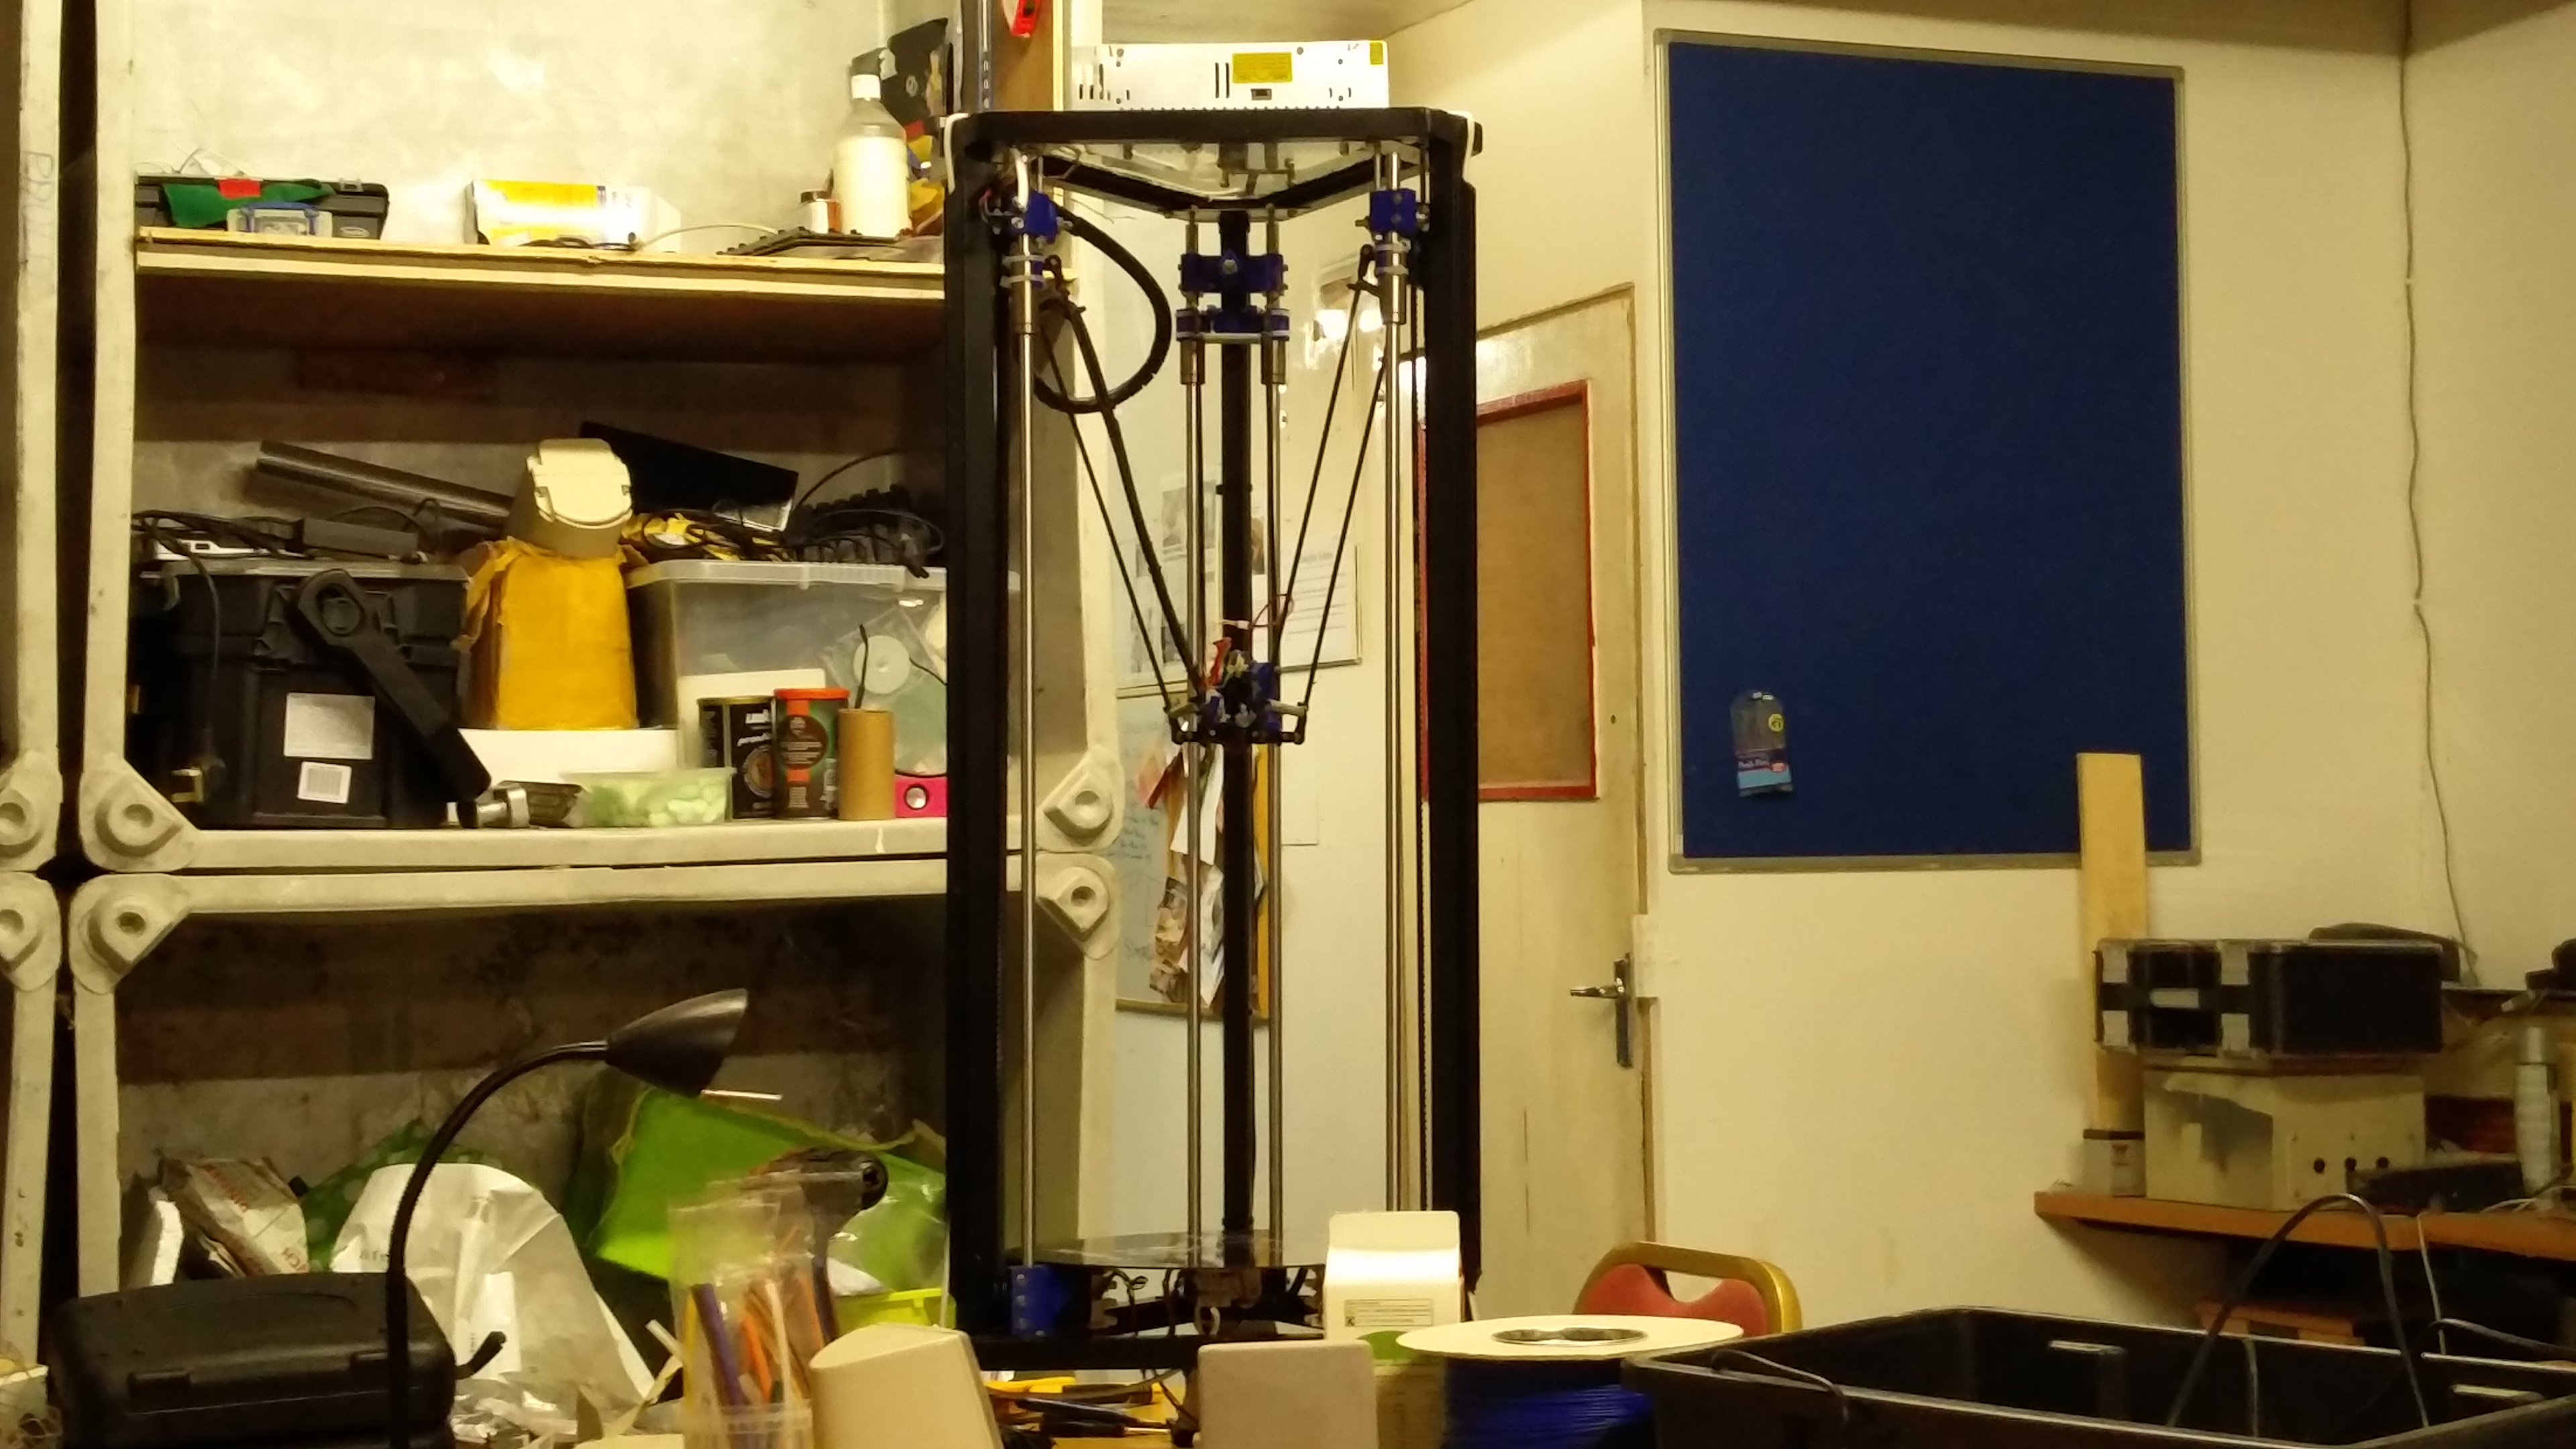
\includegraphics[width = 1.3in]{images/3dprinter_6}} 
	\end{tabular}
	\caption{Upgrading the 3D Printer 2017}
\end{figure}
\end{frame}


\section{Bartop Gaming Arcade}
\begin{frame}{Bartop Gaming Arcade}
	\begin{figure}
		\begin{tabular}{ccc}
			\subfloat{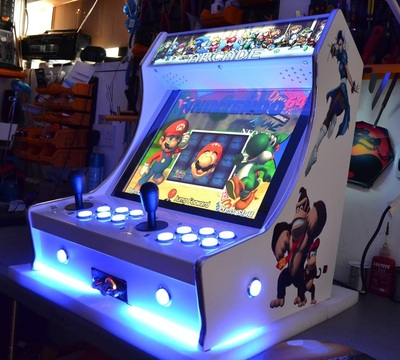
\includegraphics[width = 1.3in]{images/gaming_1}} &
			\subfloat{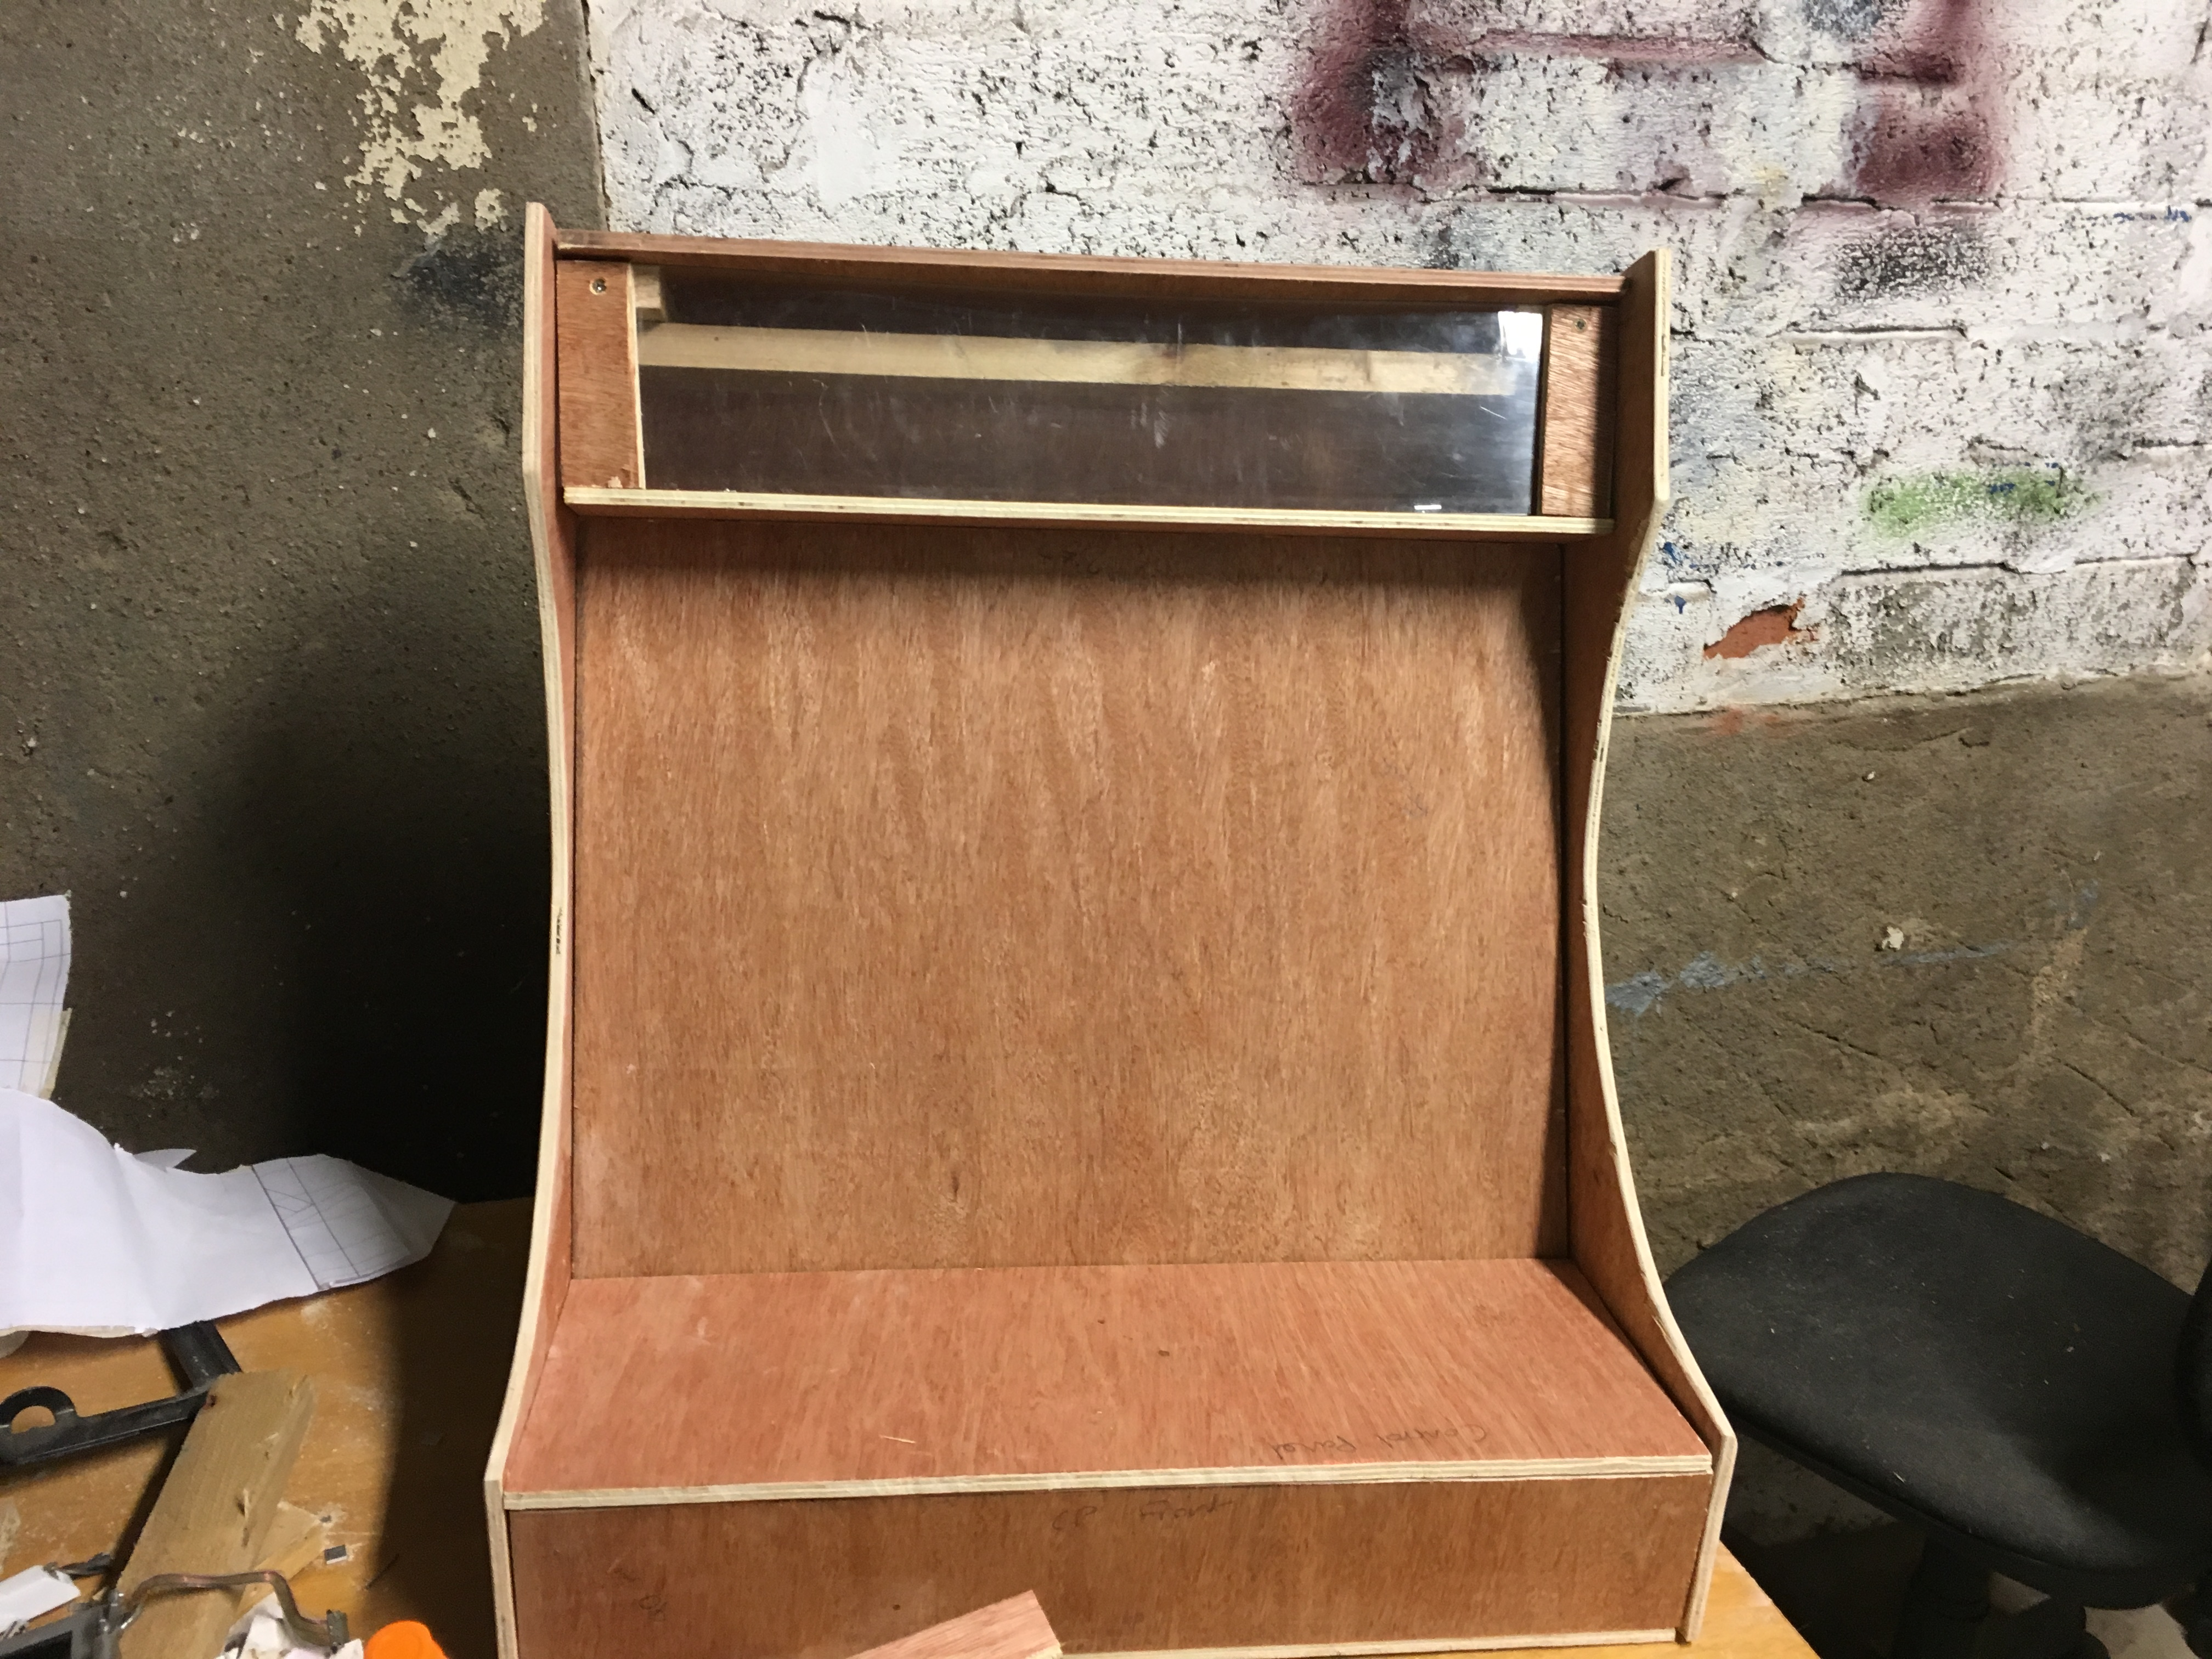
\includegraphics[width = 1.3in]{images/gaming_2}} &
			\subfloat{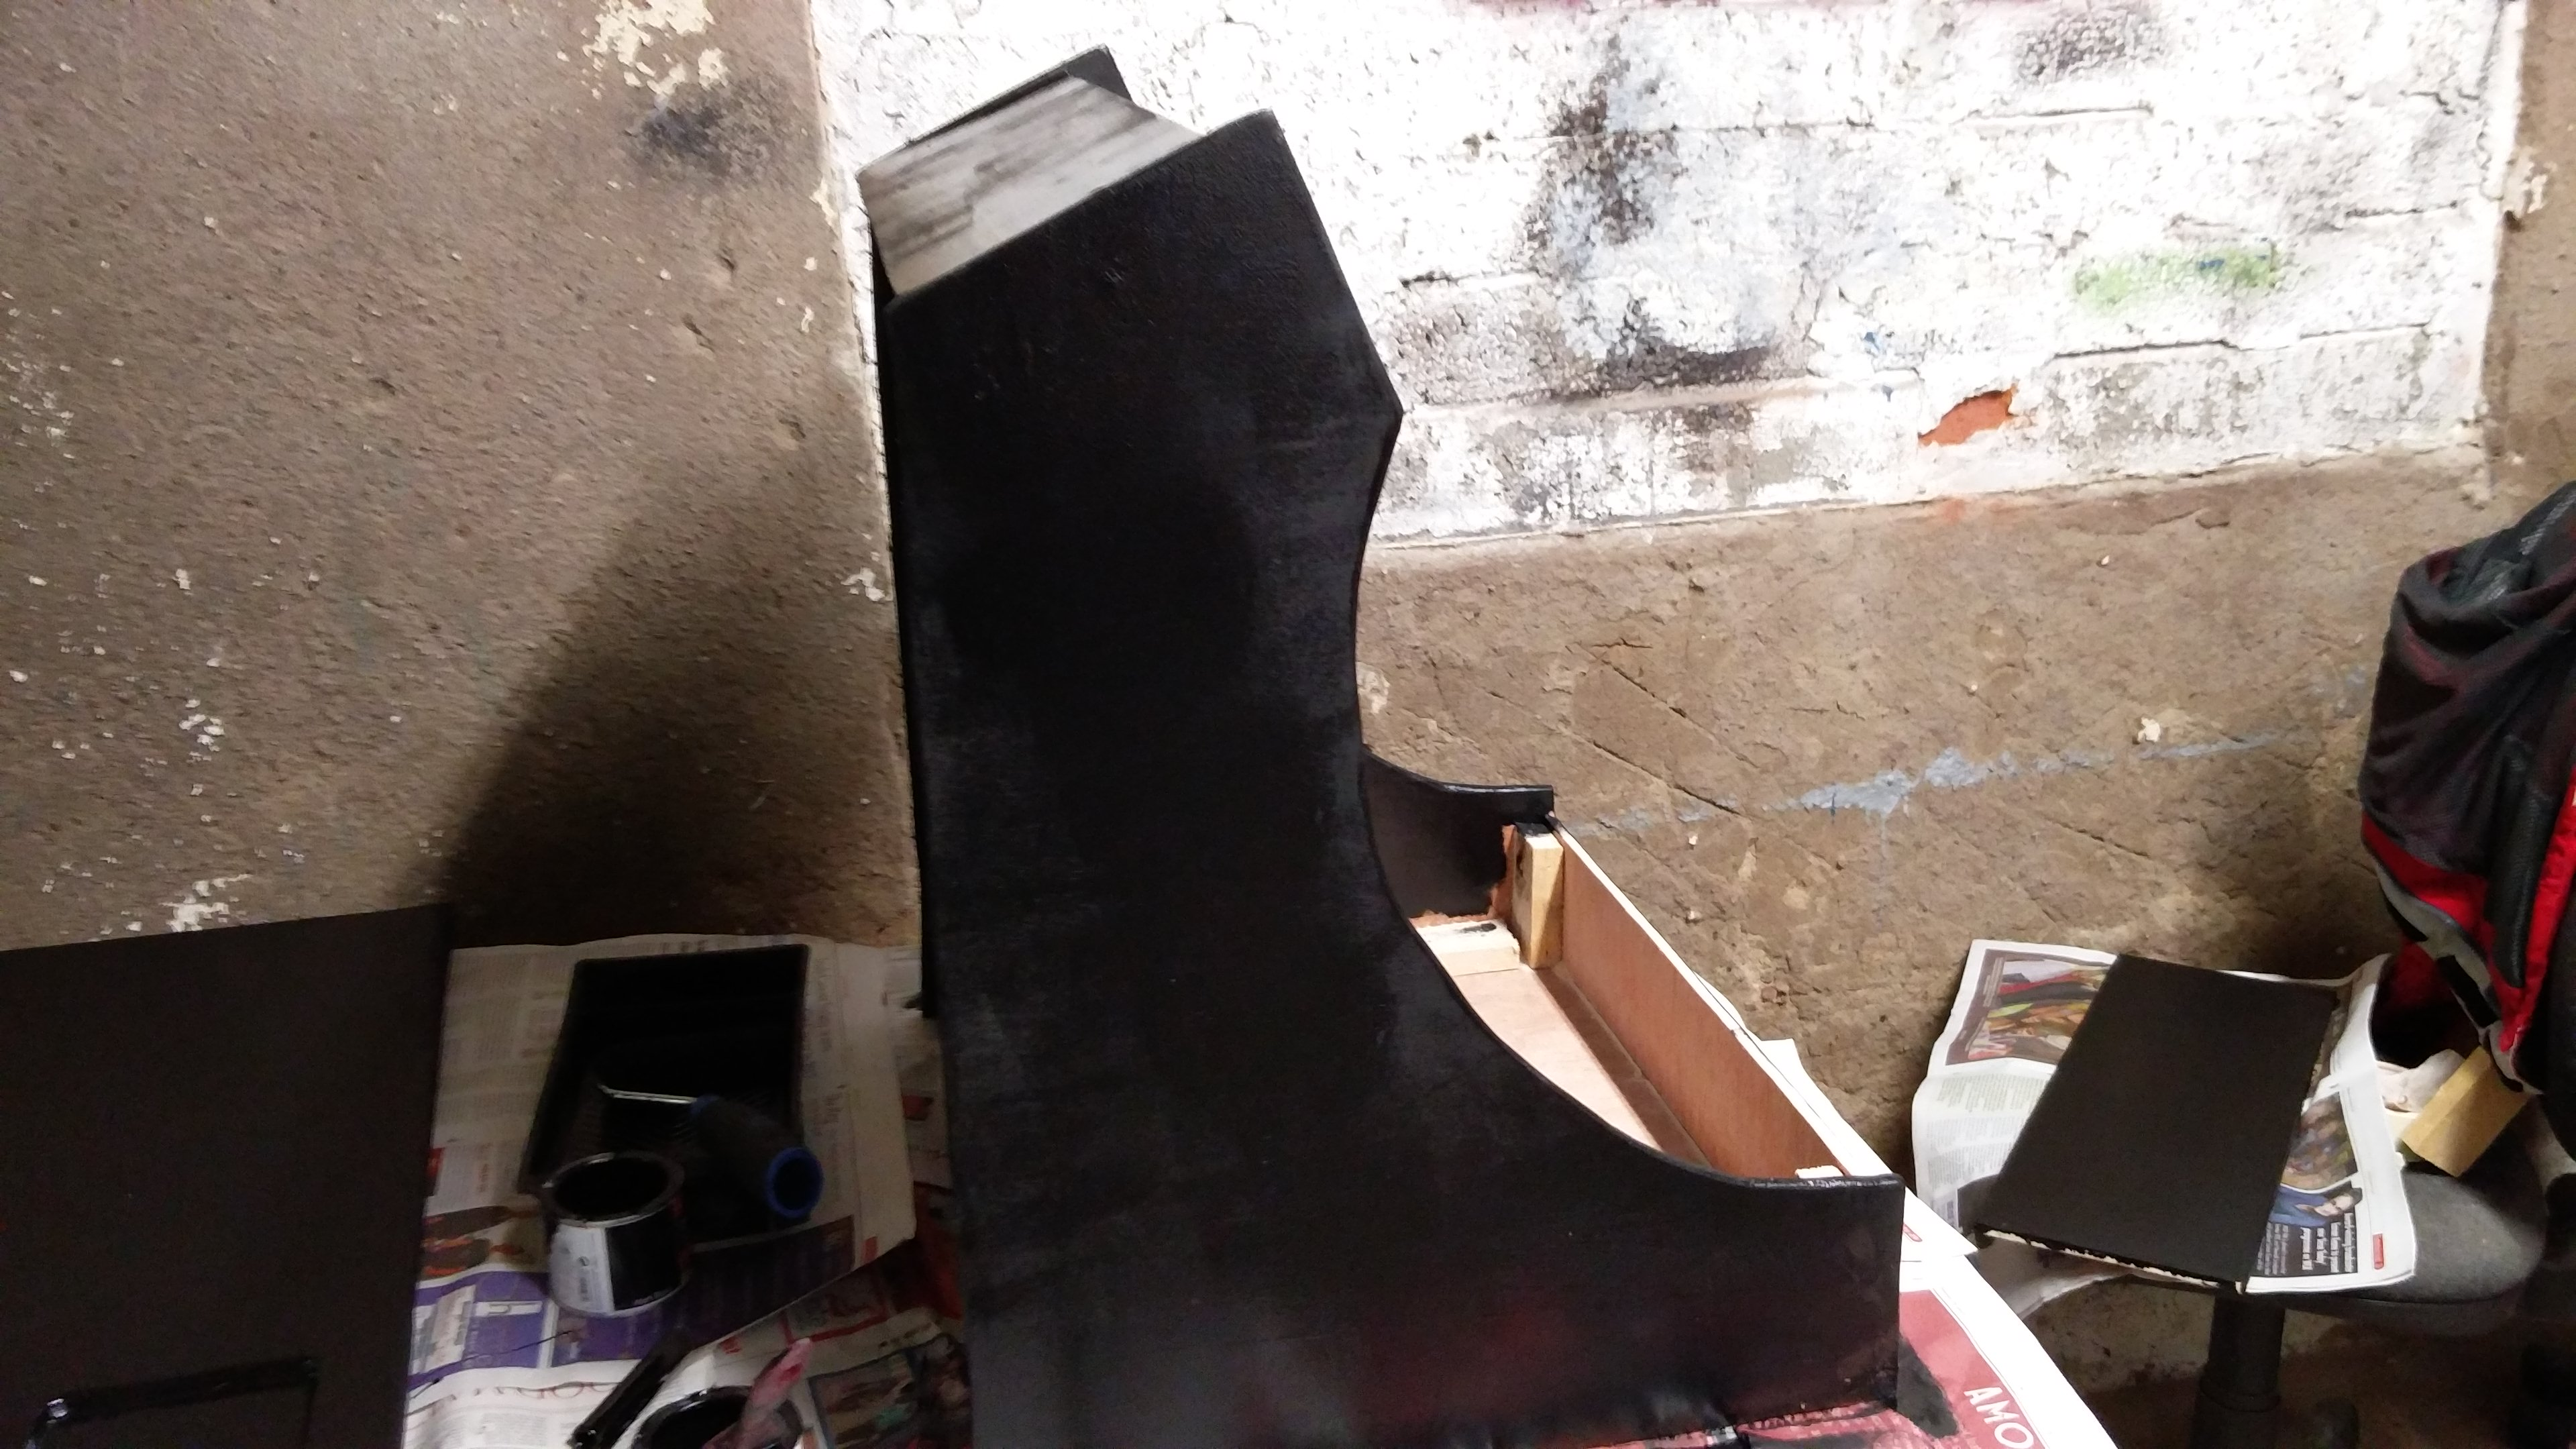
\includegraphics[width = 1.3in]{images/gaming_3}} \\
			\subfloat{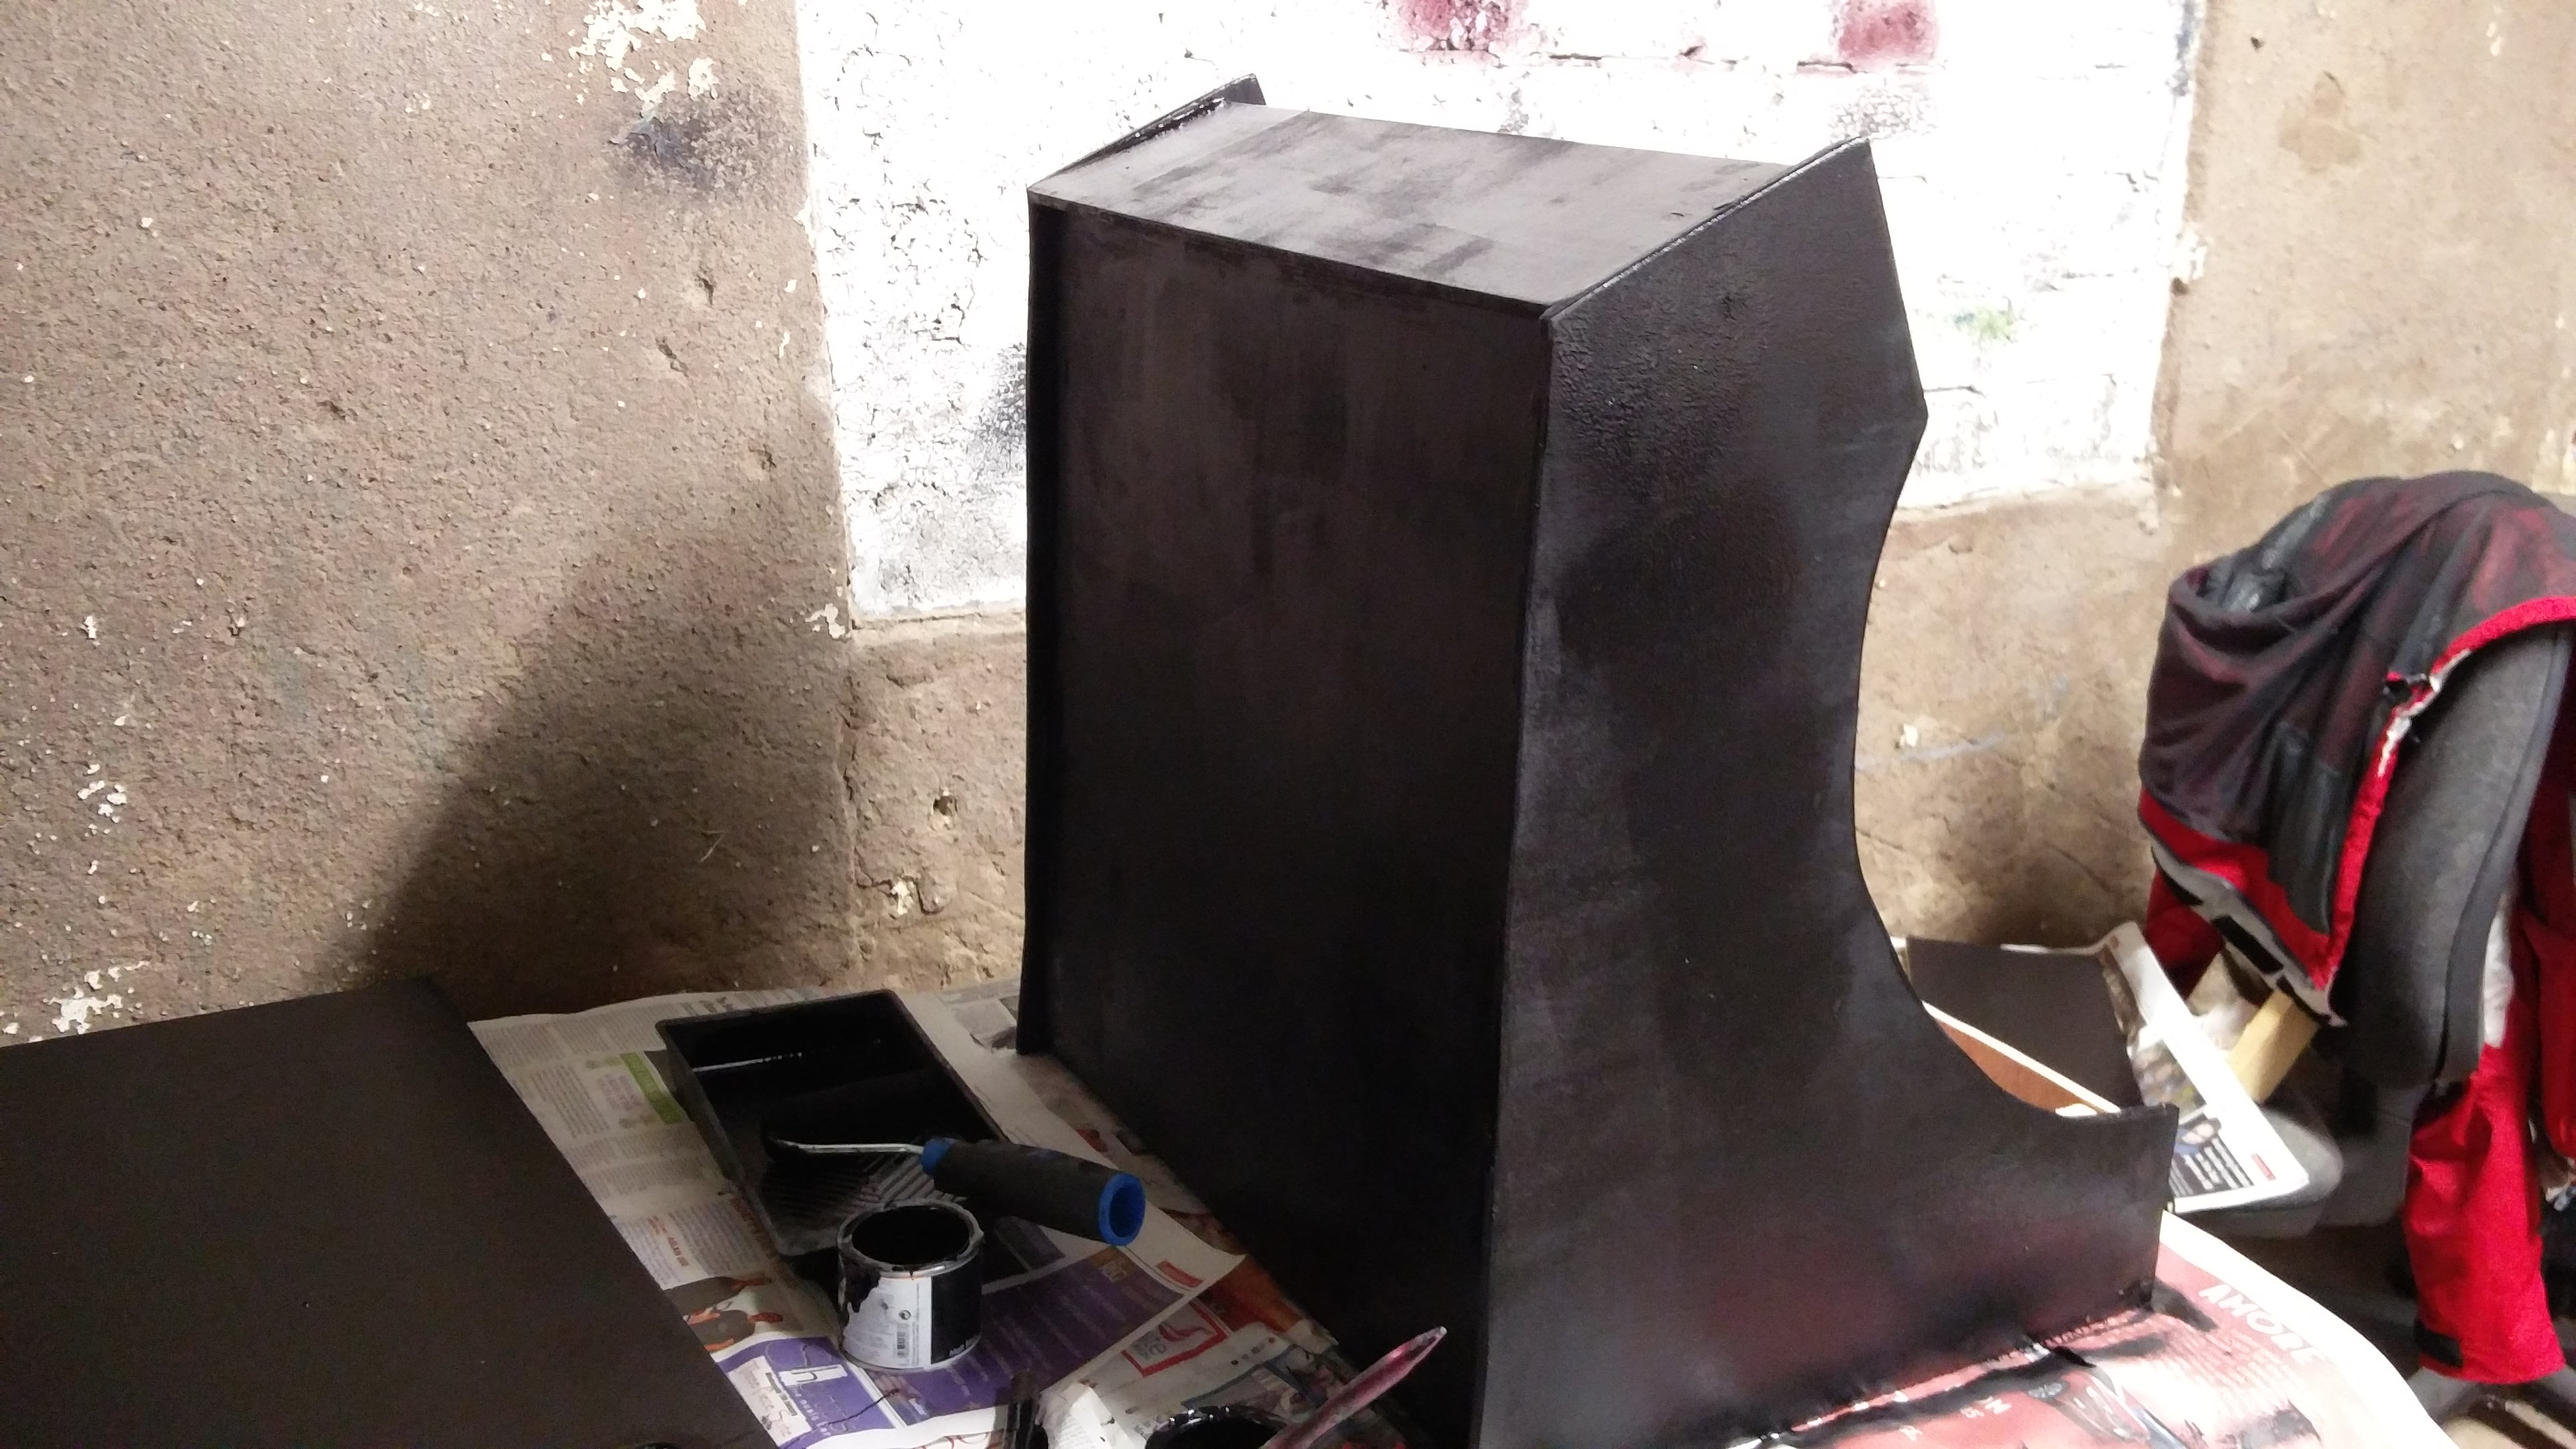
\includegraphics[width = 1.3in]{images/gaming_4}} &    \subfloat{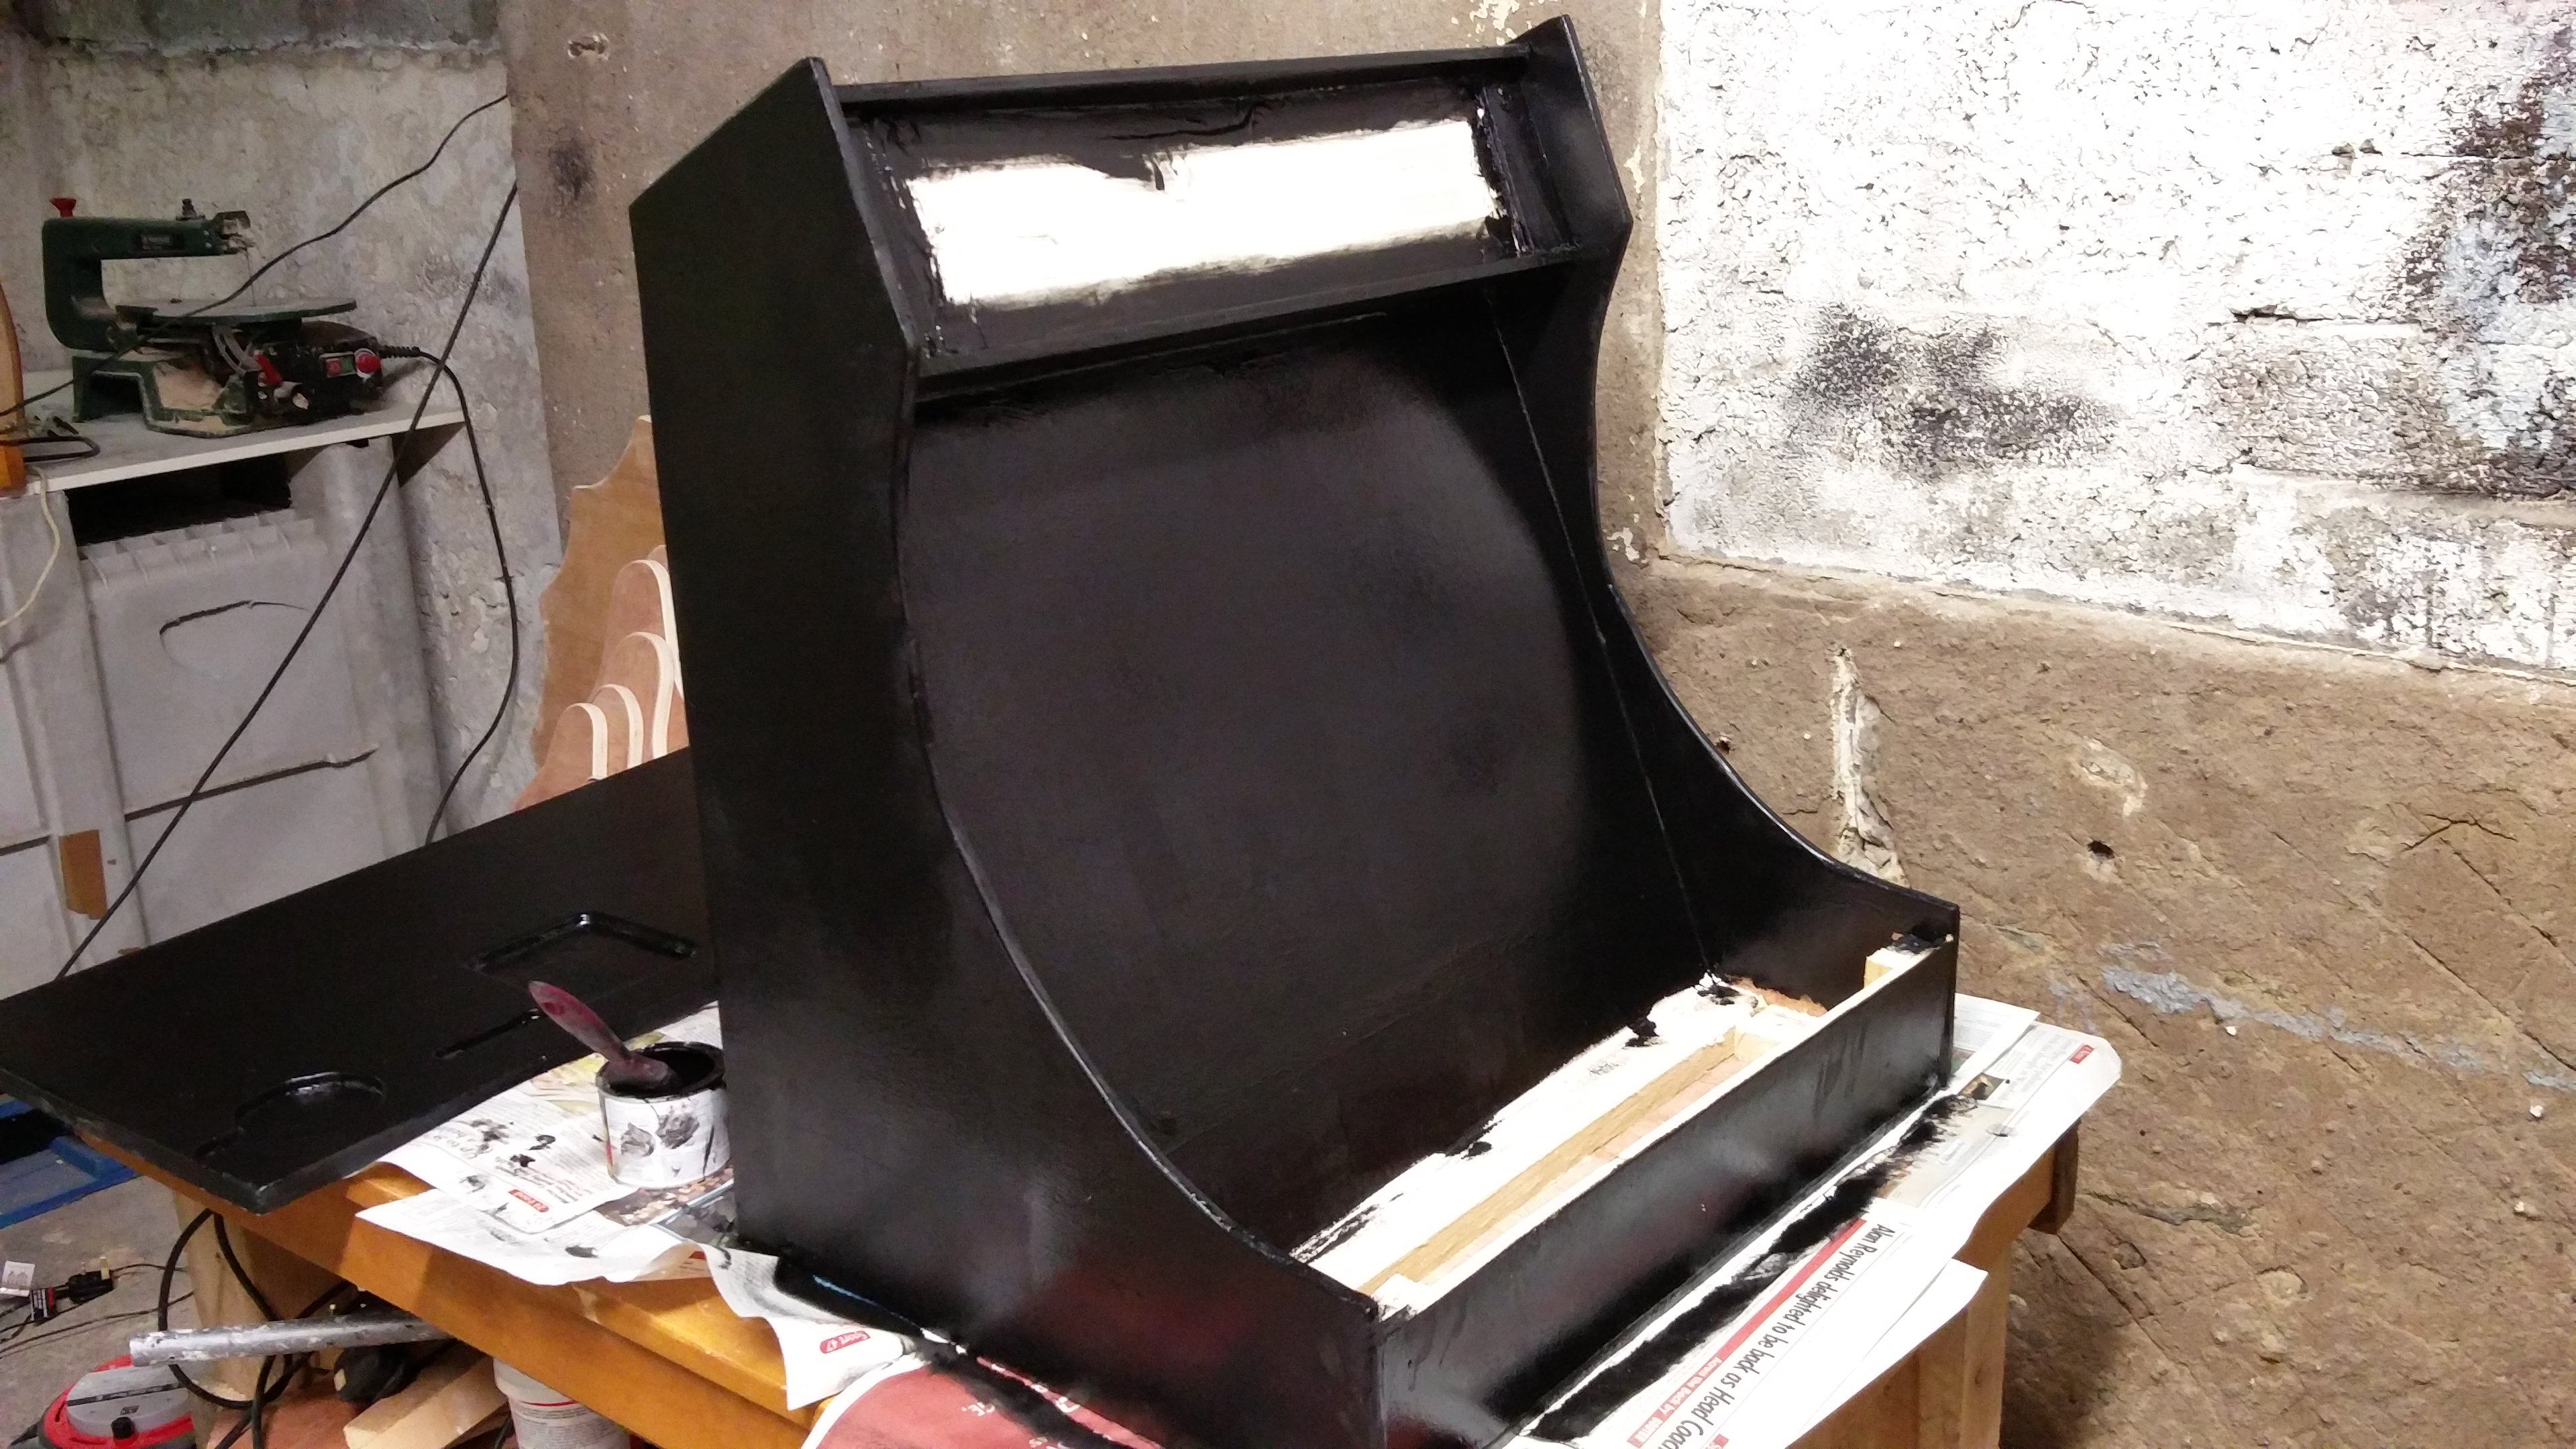
\includegraphics[width = 1.3in]{images/gaming_5}} &
			\subfloat{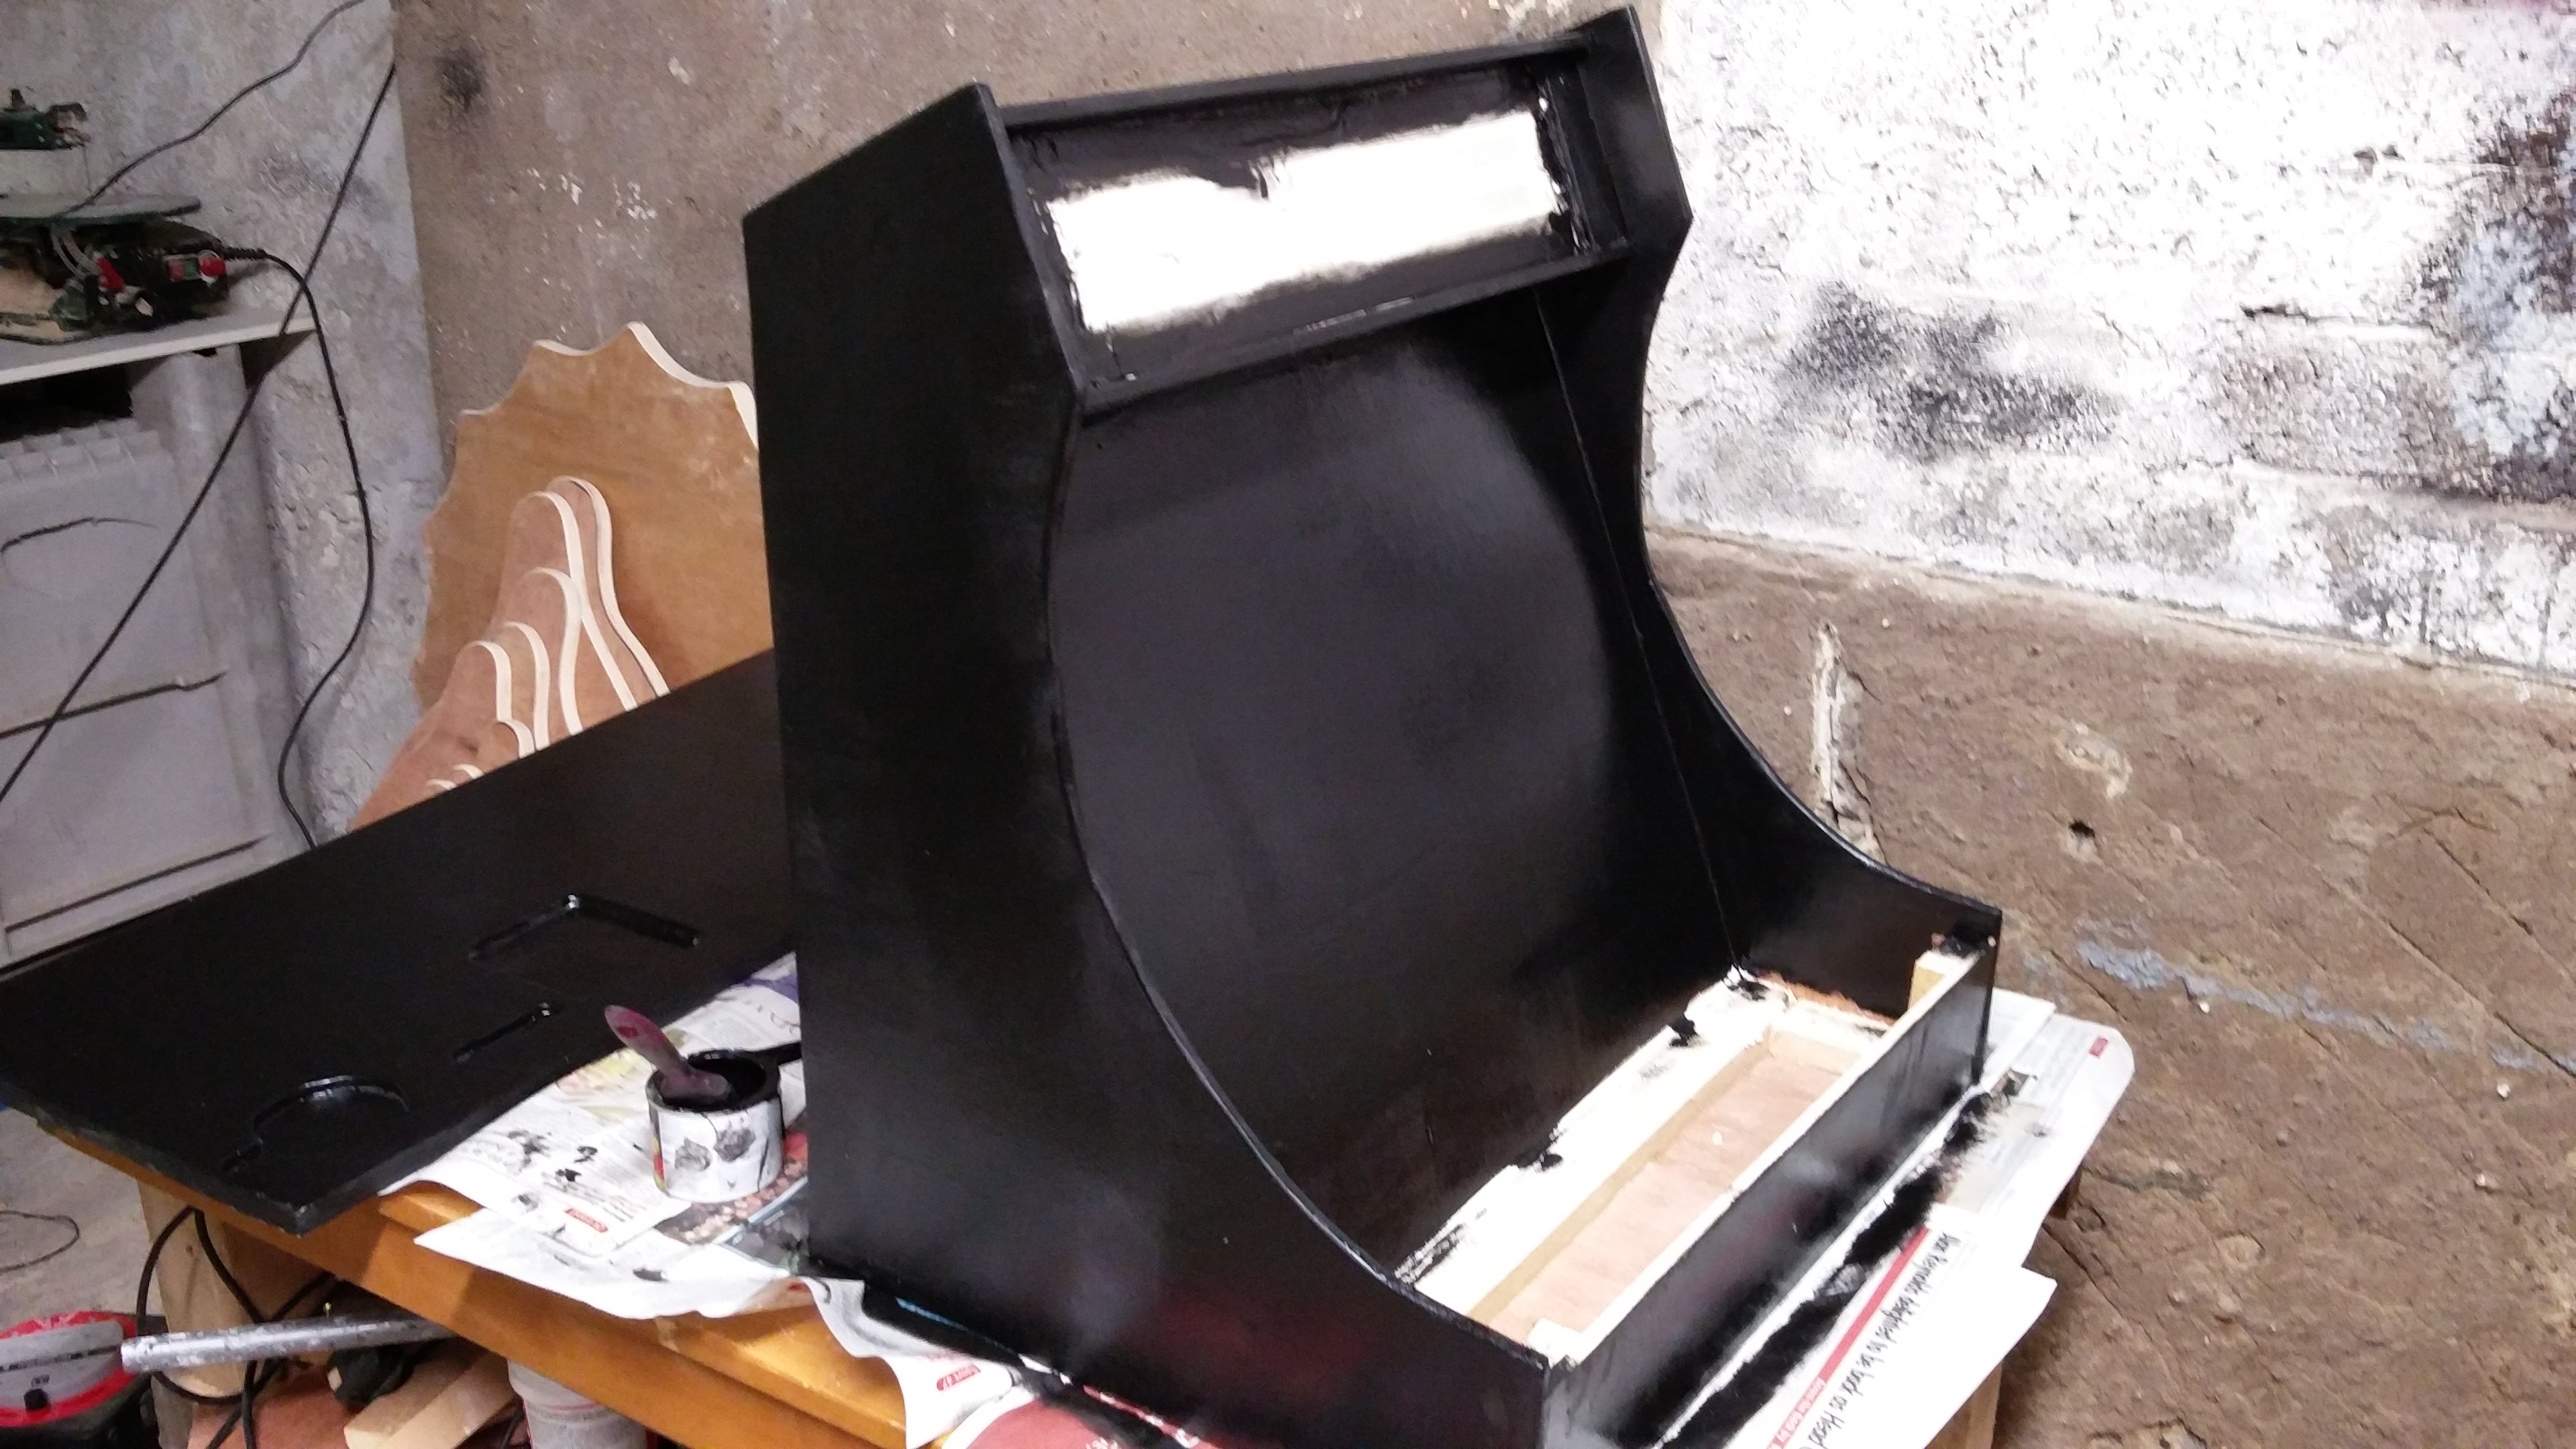
\includegraphics[width = 1.3in]{images/gaming_6}} 
		\end{tabular}
		\caption{Bartop Gaming Arcade 2017}
	\end{figure}
\end{frame}


\section{Jigsaw Dinosaurs}
\begin{frame}{Jigsaw Dinosaurs}
	\begin{figure}
		\begin{tabular}{ccc}
			\subfloat{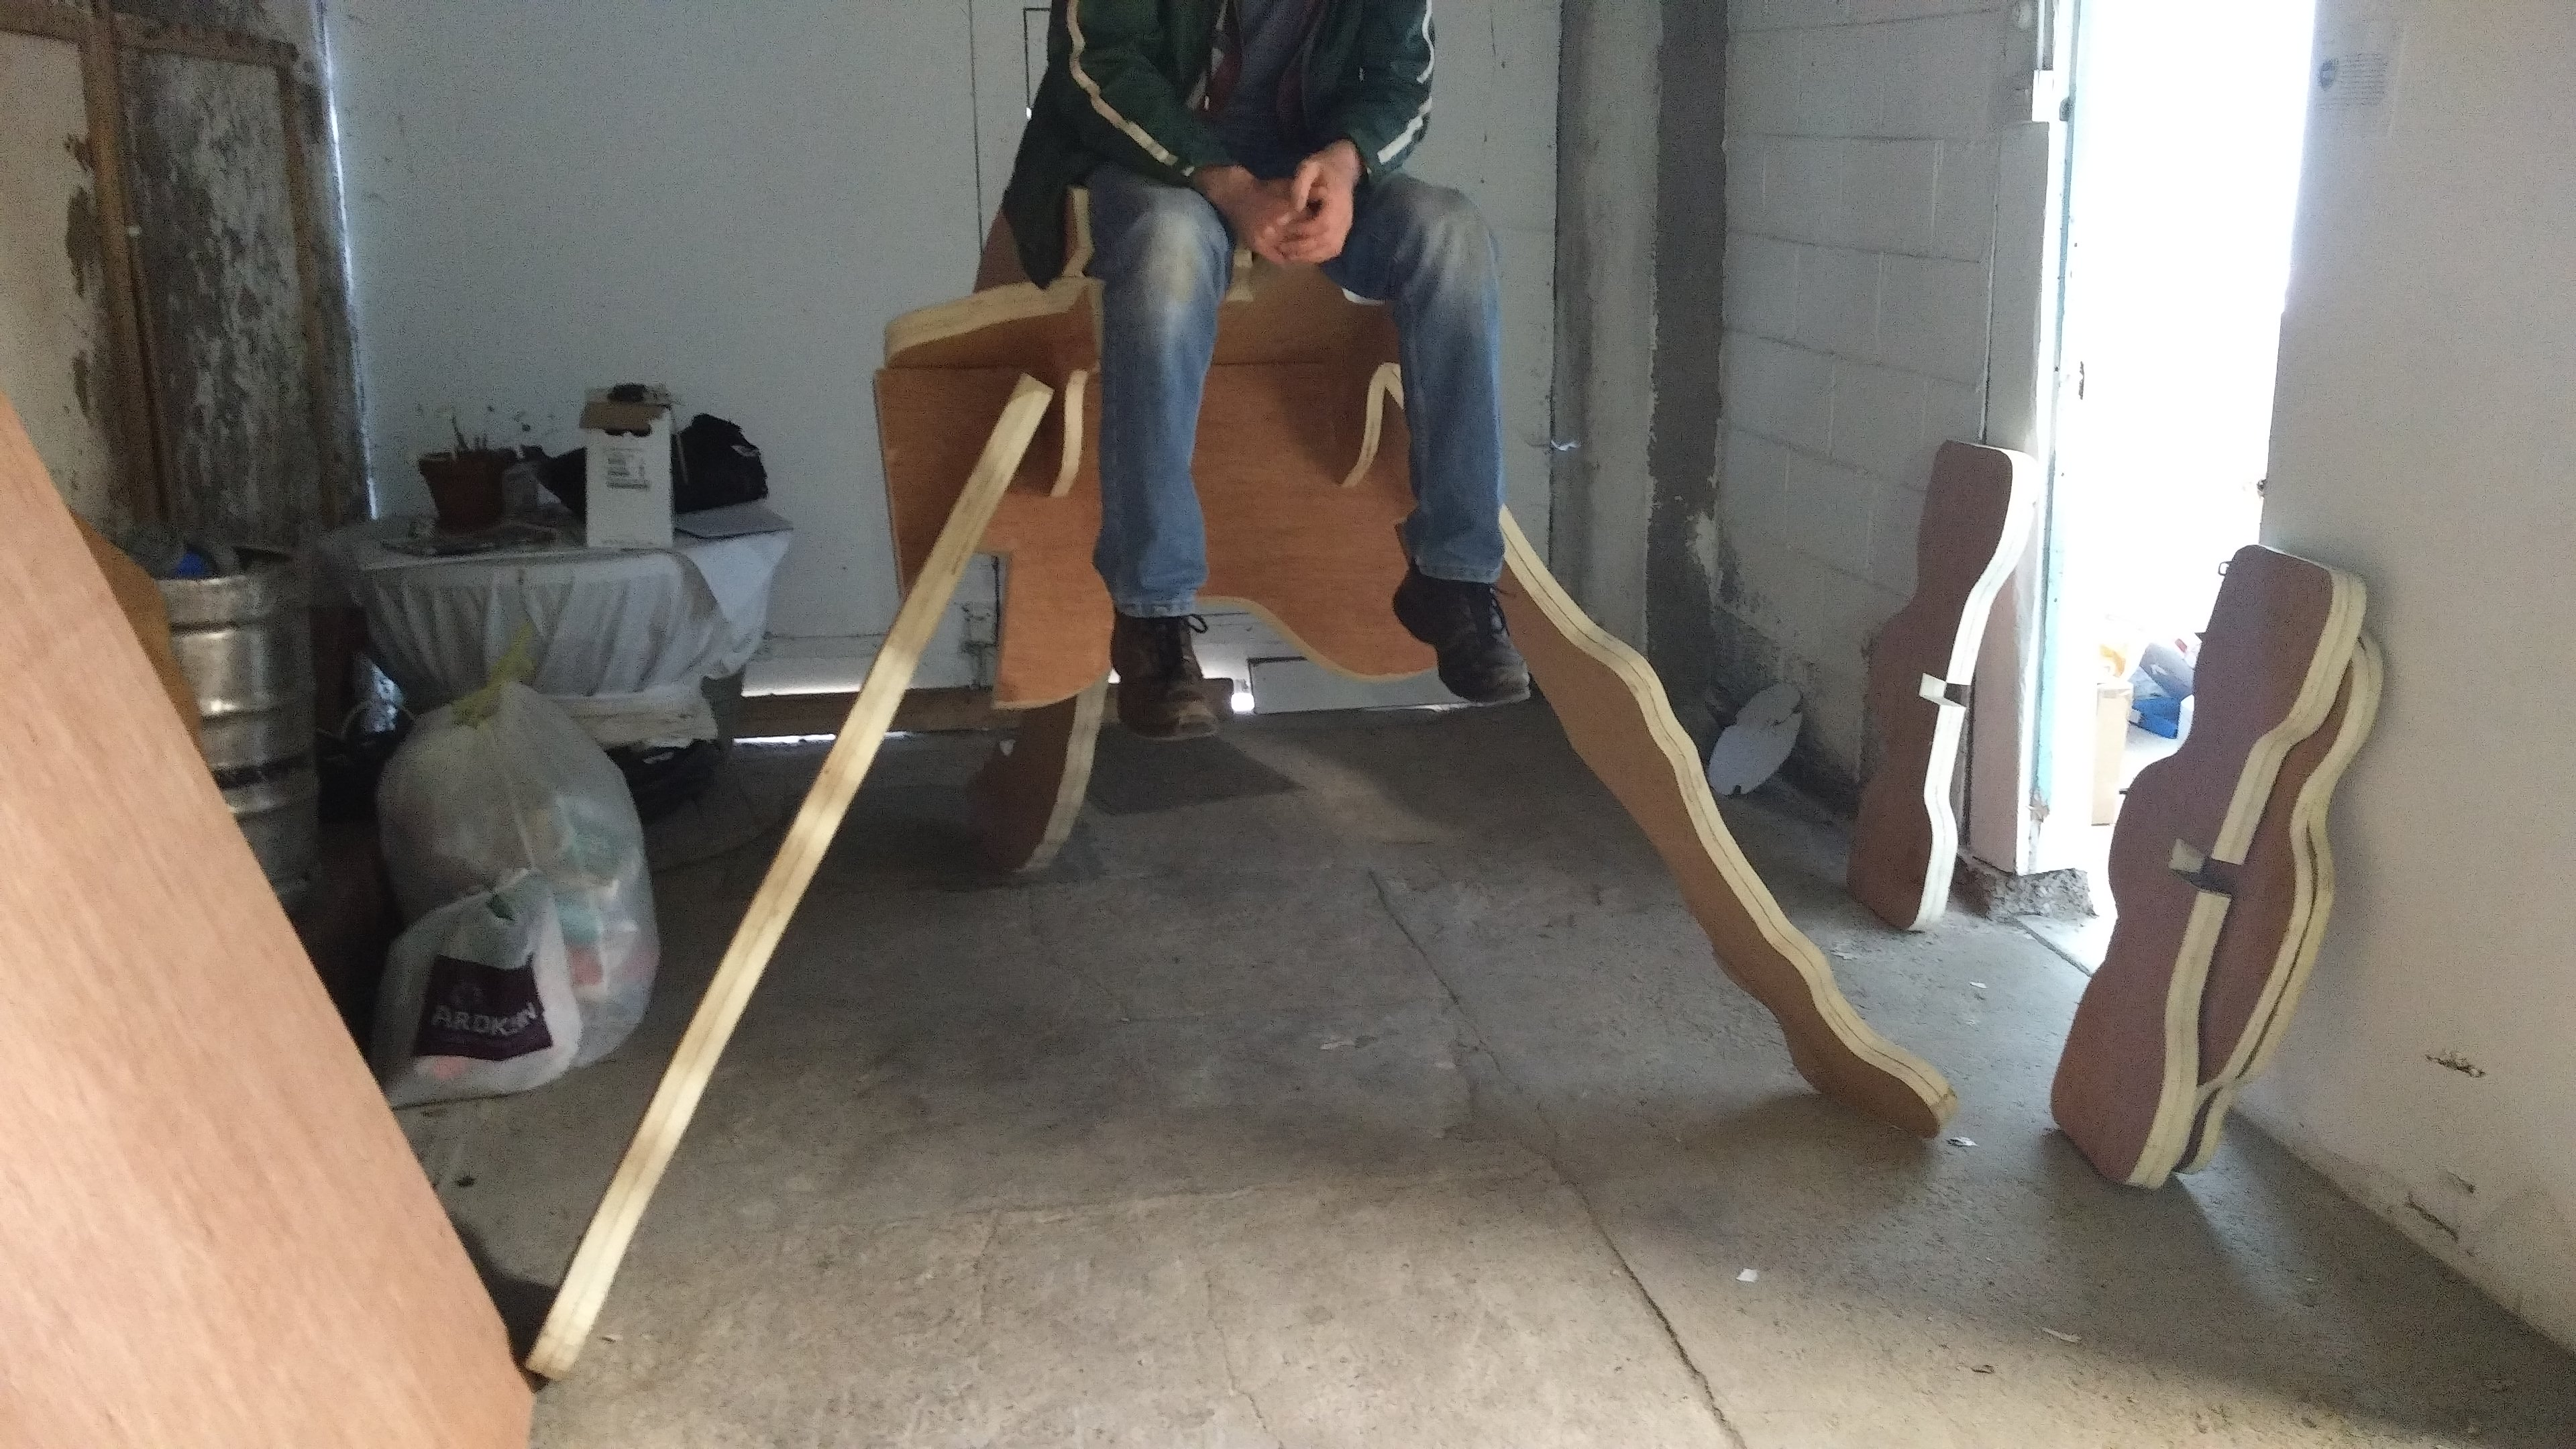
\includegraphics[width = 1.3in]{images/jig_1}} &
			\subfloat{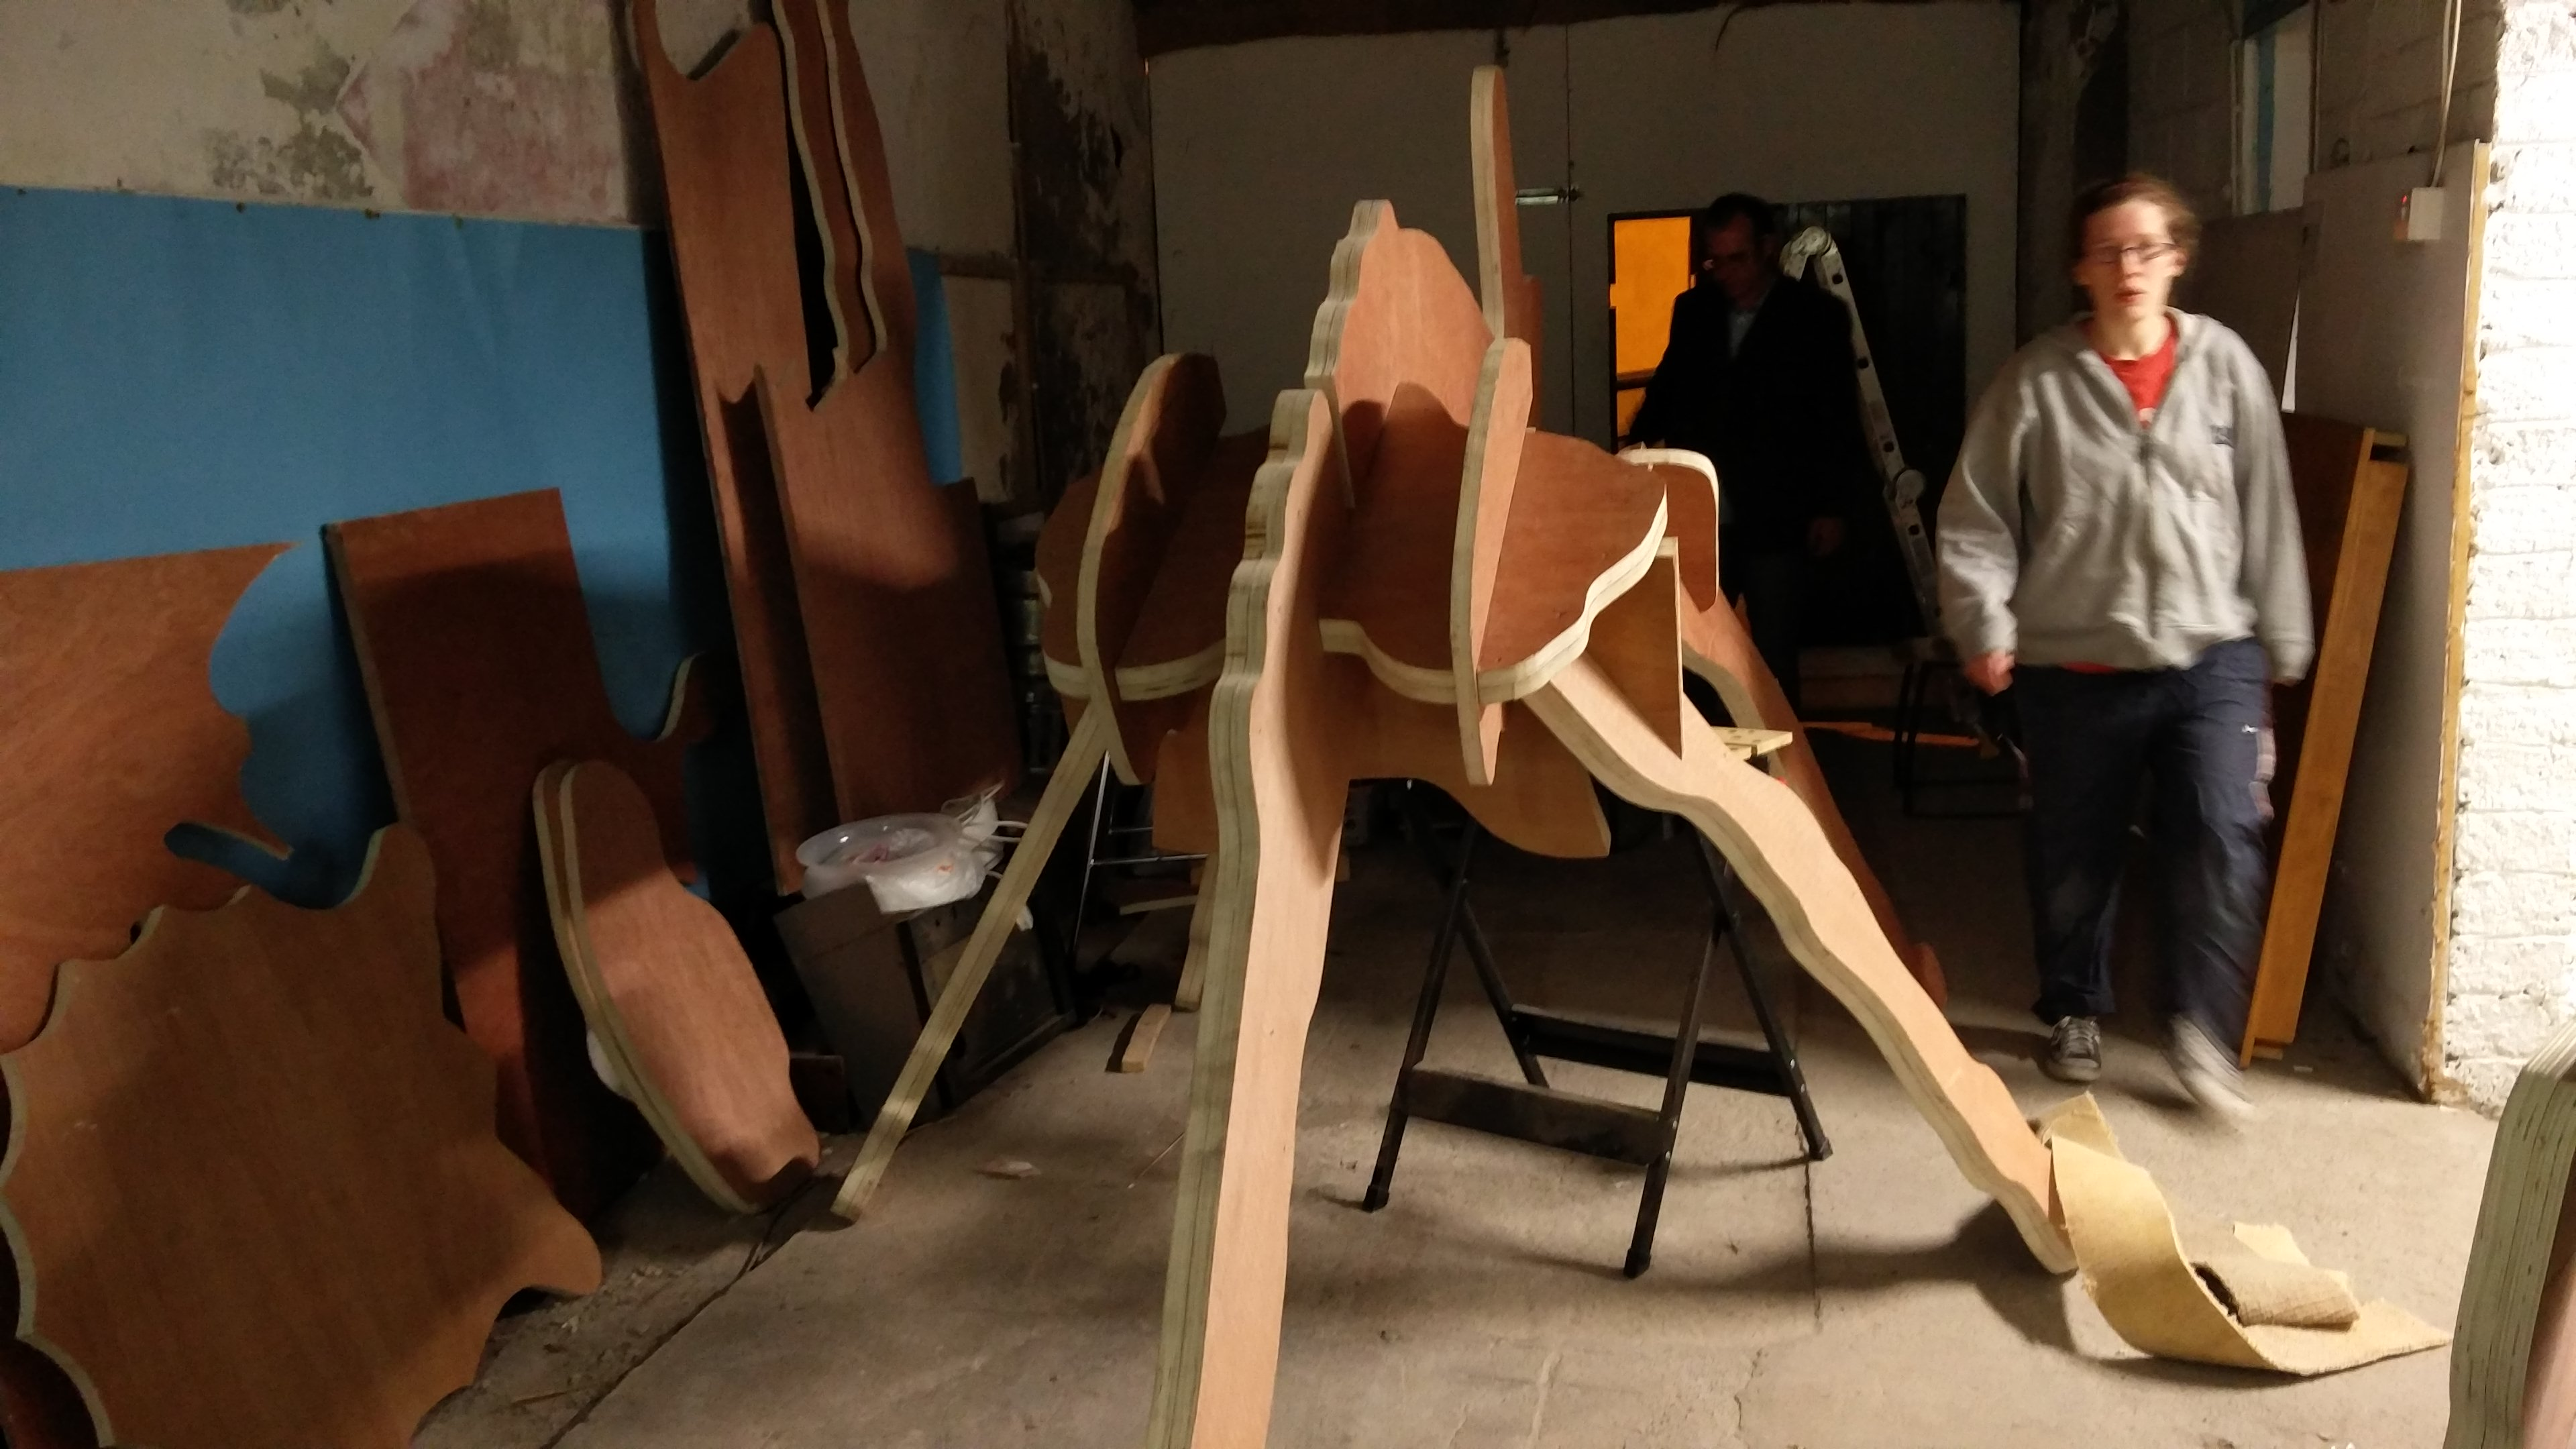
\includegraphics[width = 1.3in]{images/jig_2}} &
			\subfloat{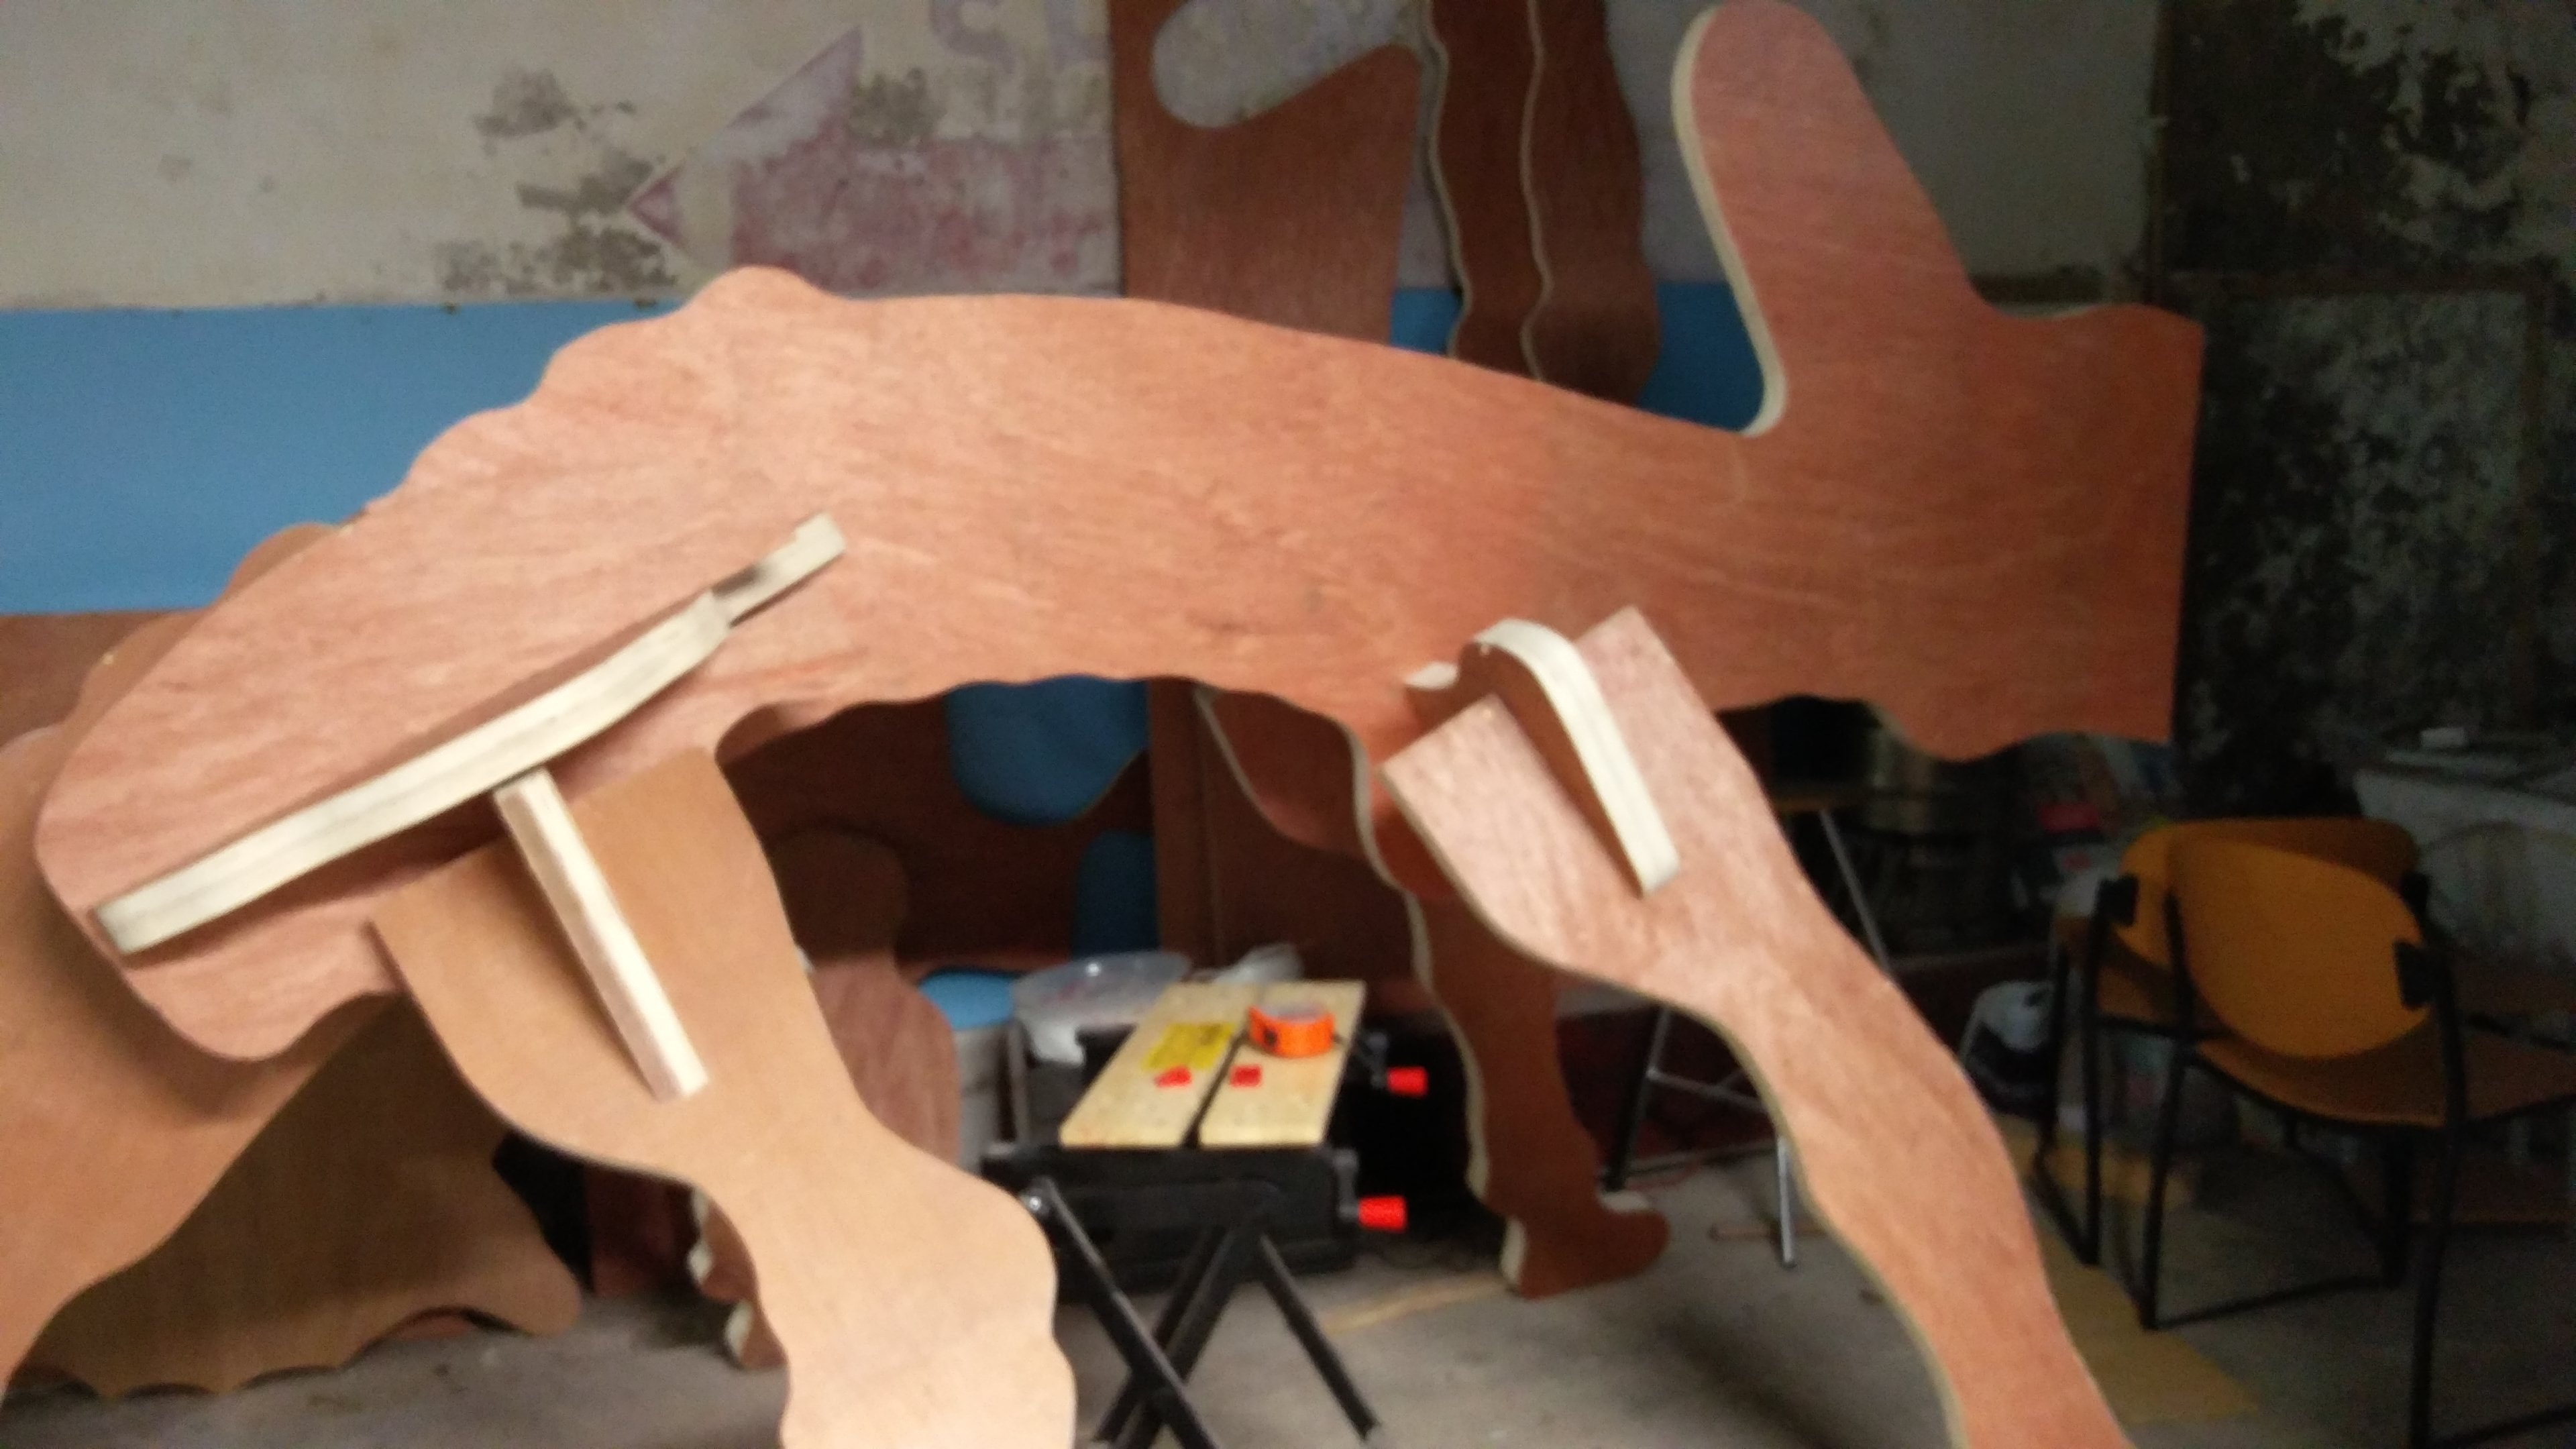
\includegraphics[width = 1.3in]{images/jig_3}} \\
			\subfloat{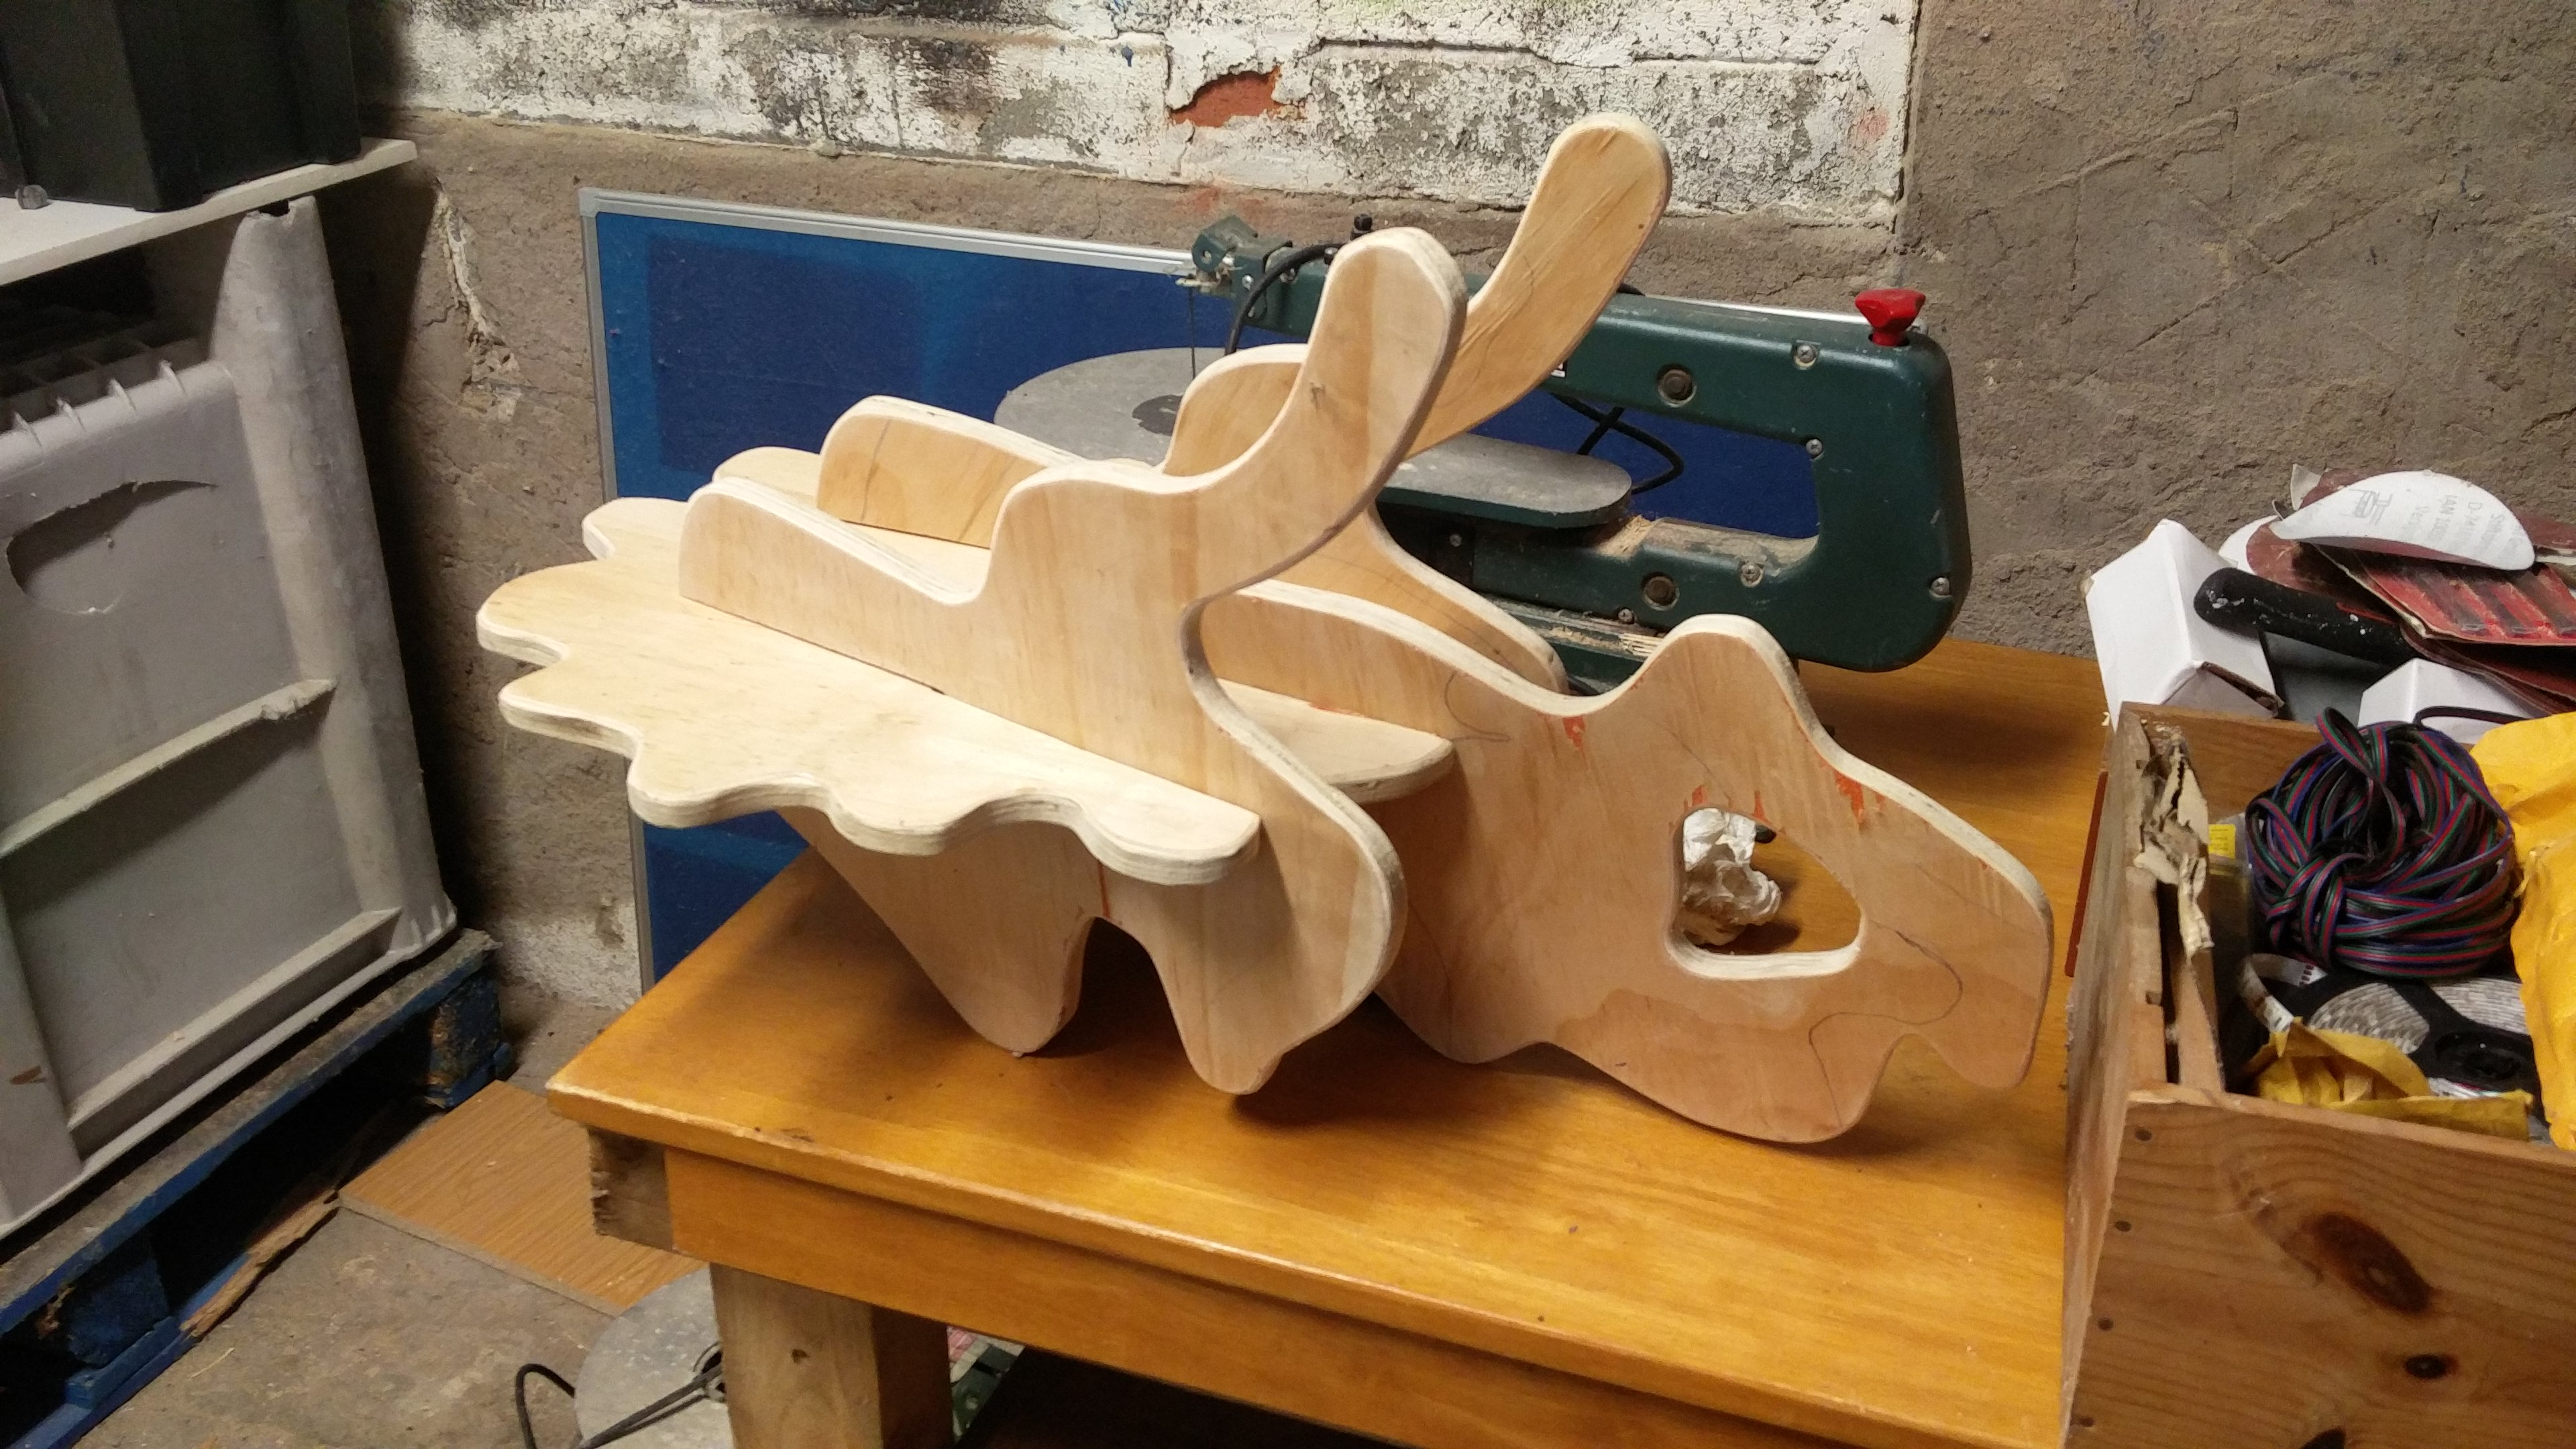
\includegraphics[width = 1.3in]{images/jig_4}} &    \subfloat{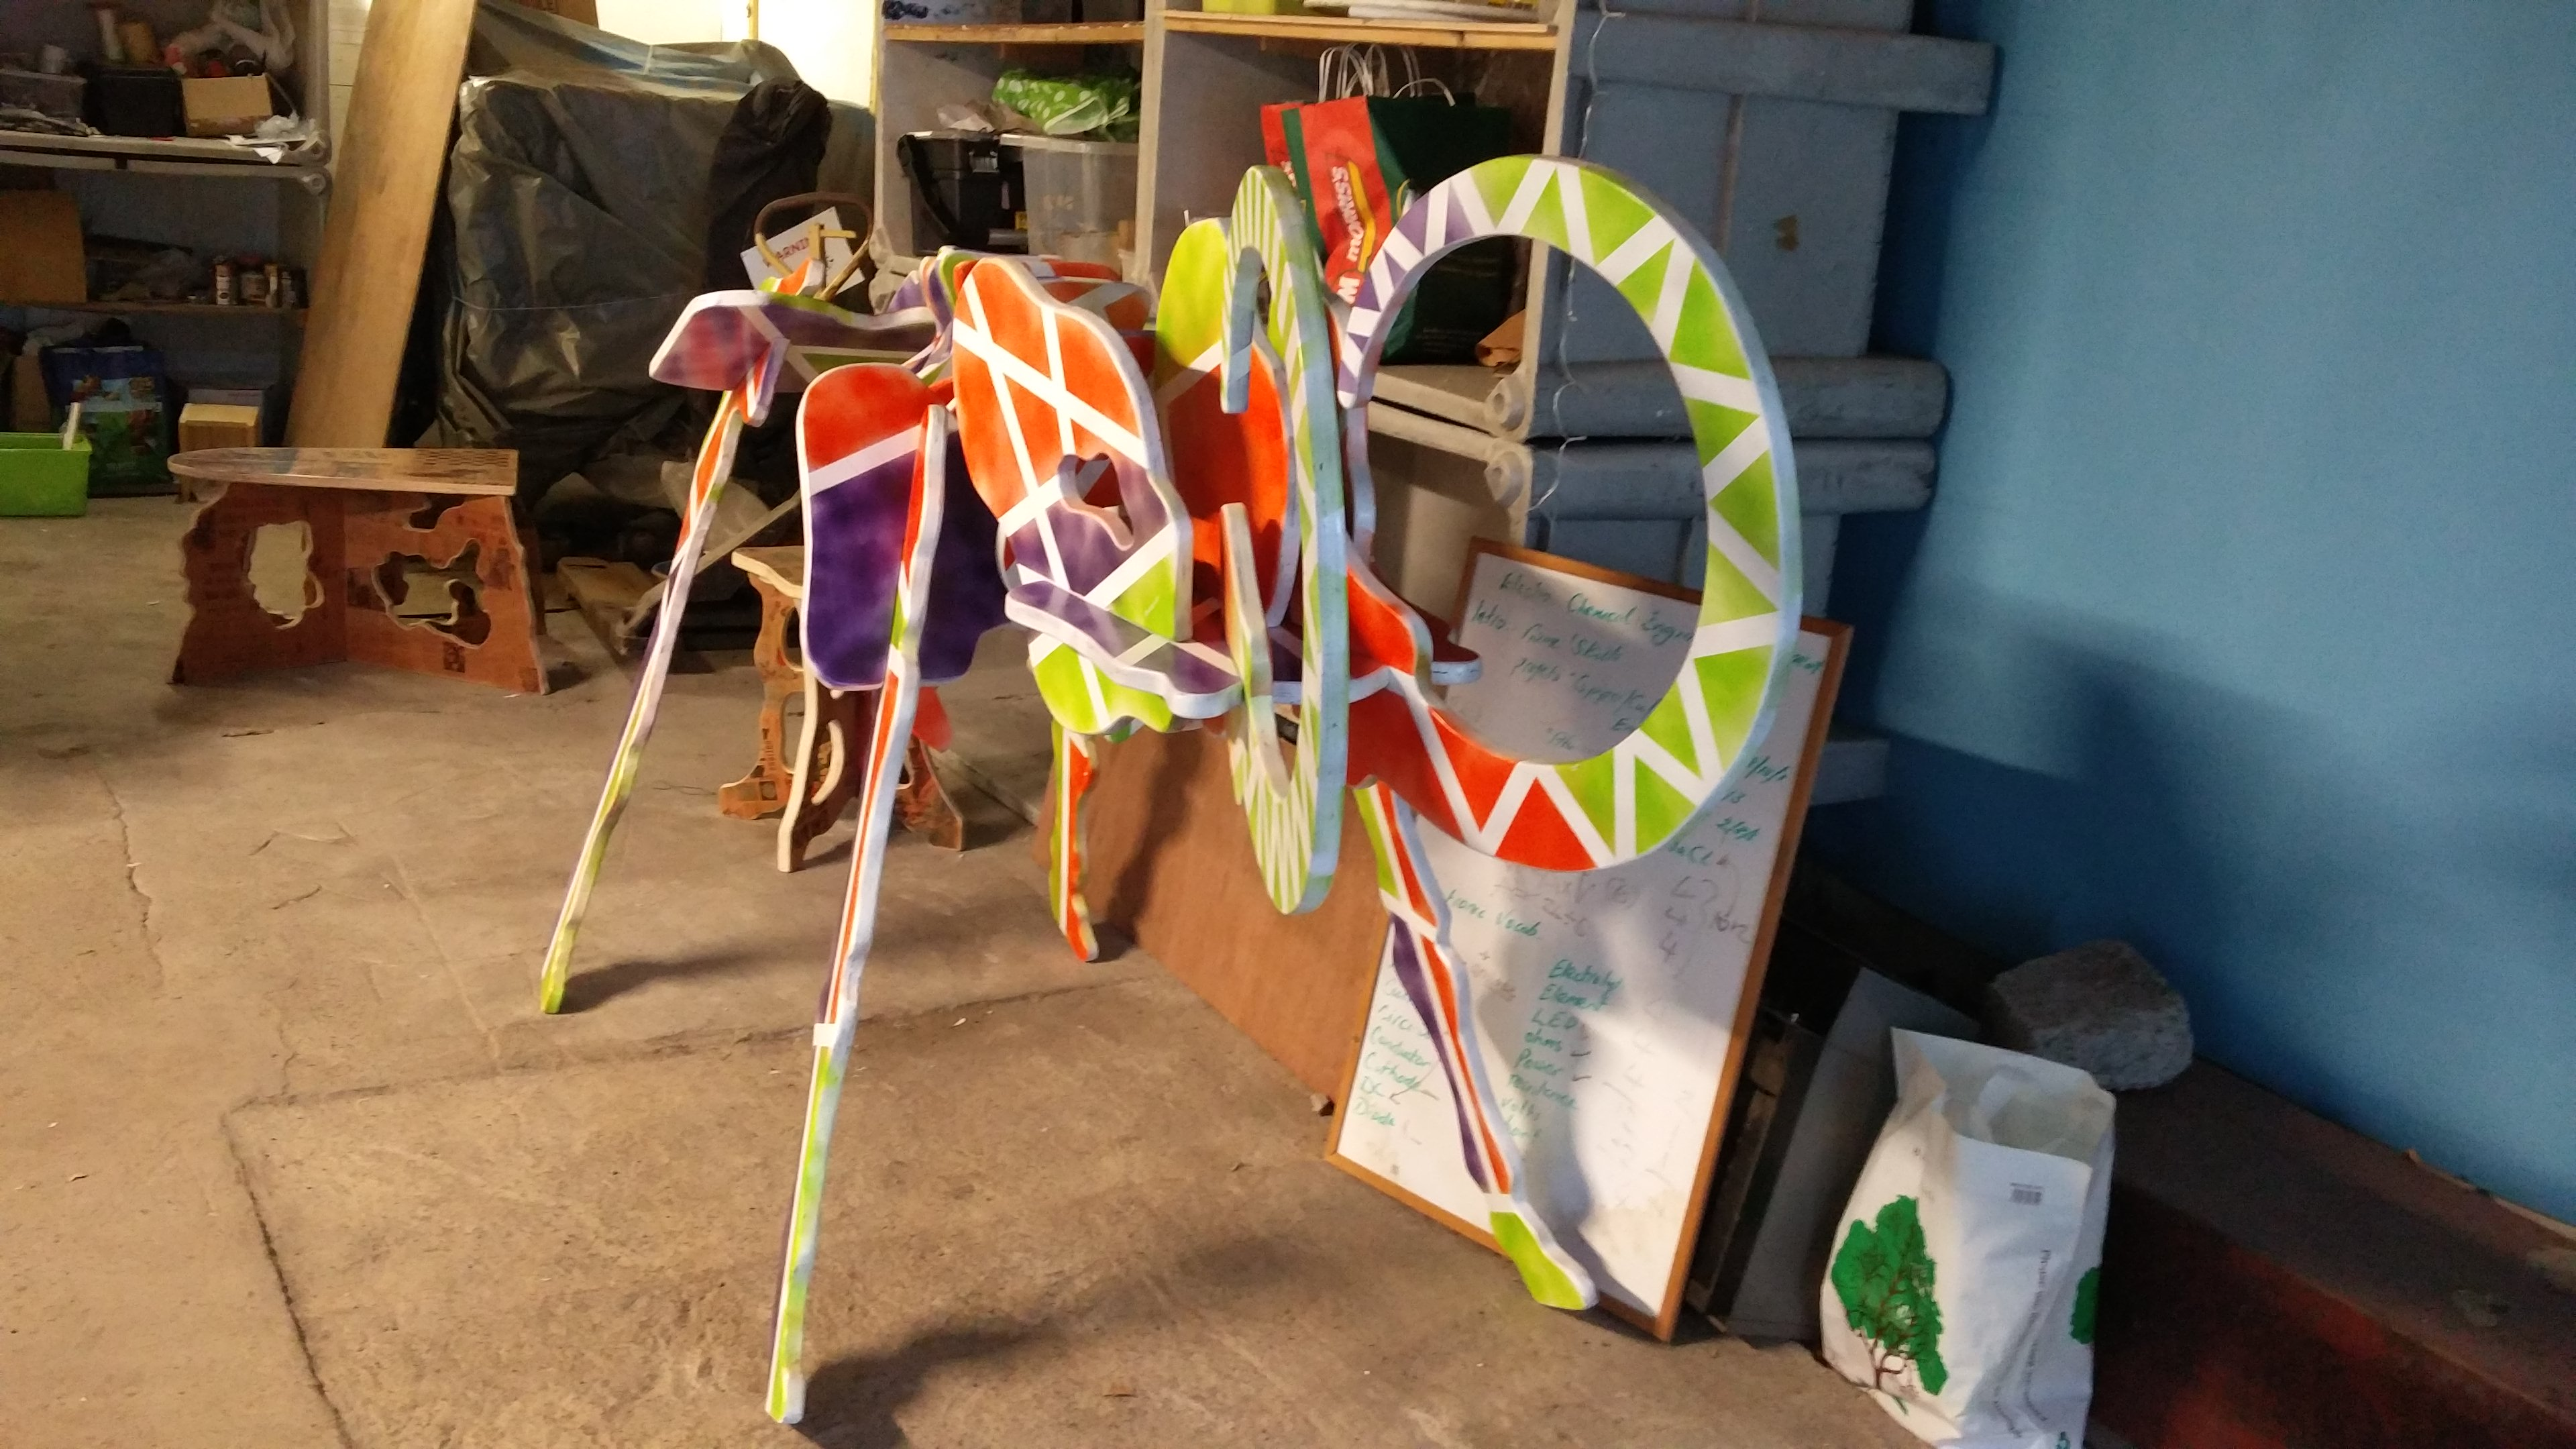
\includegraphics[width = 1.3in]{images/jig_5}} &
			\subfloat{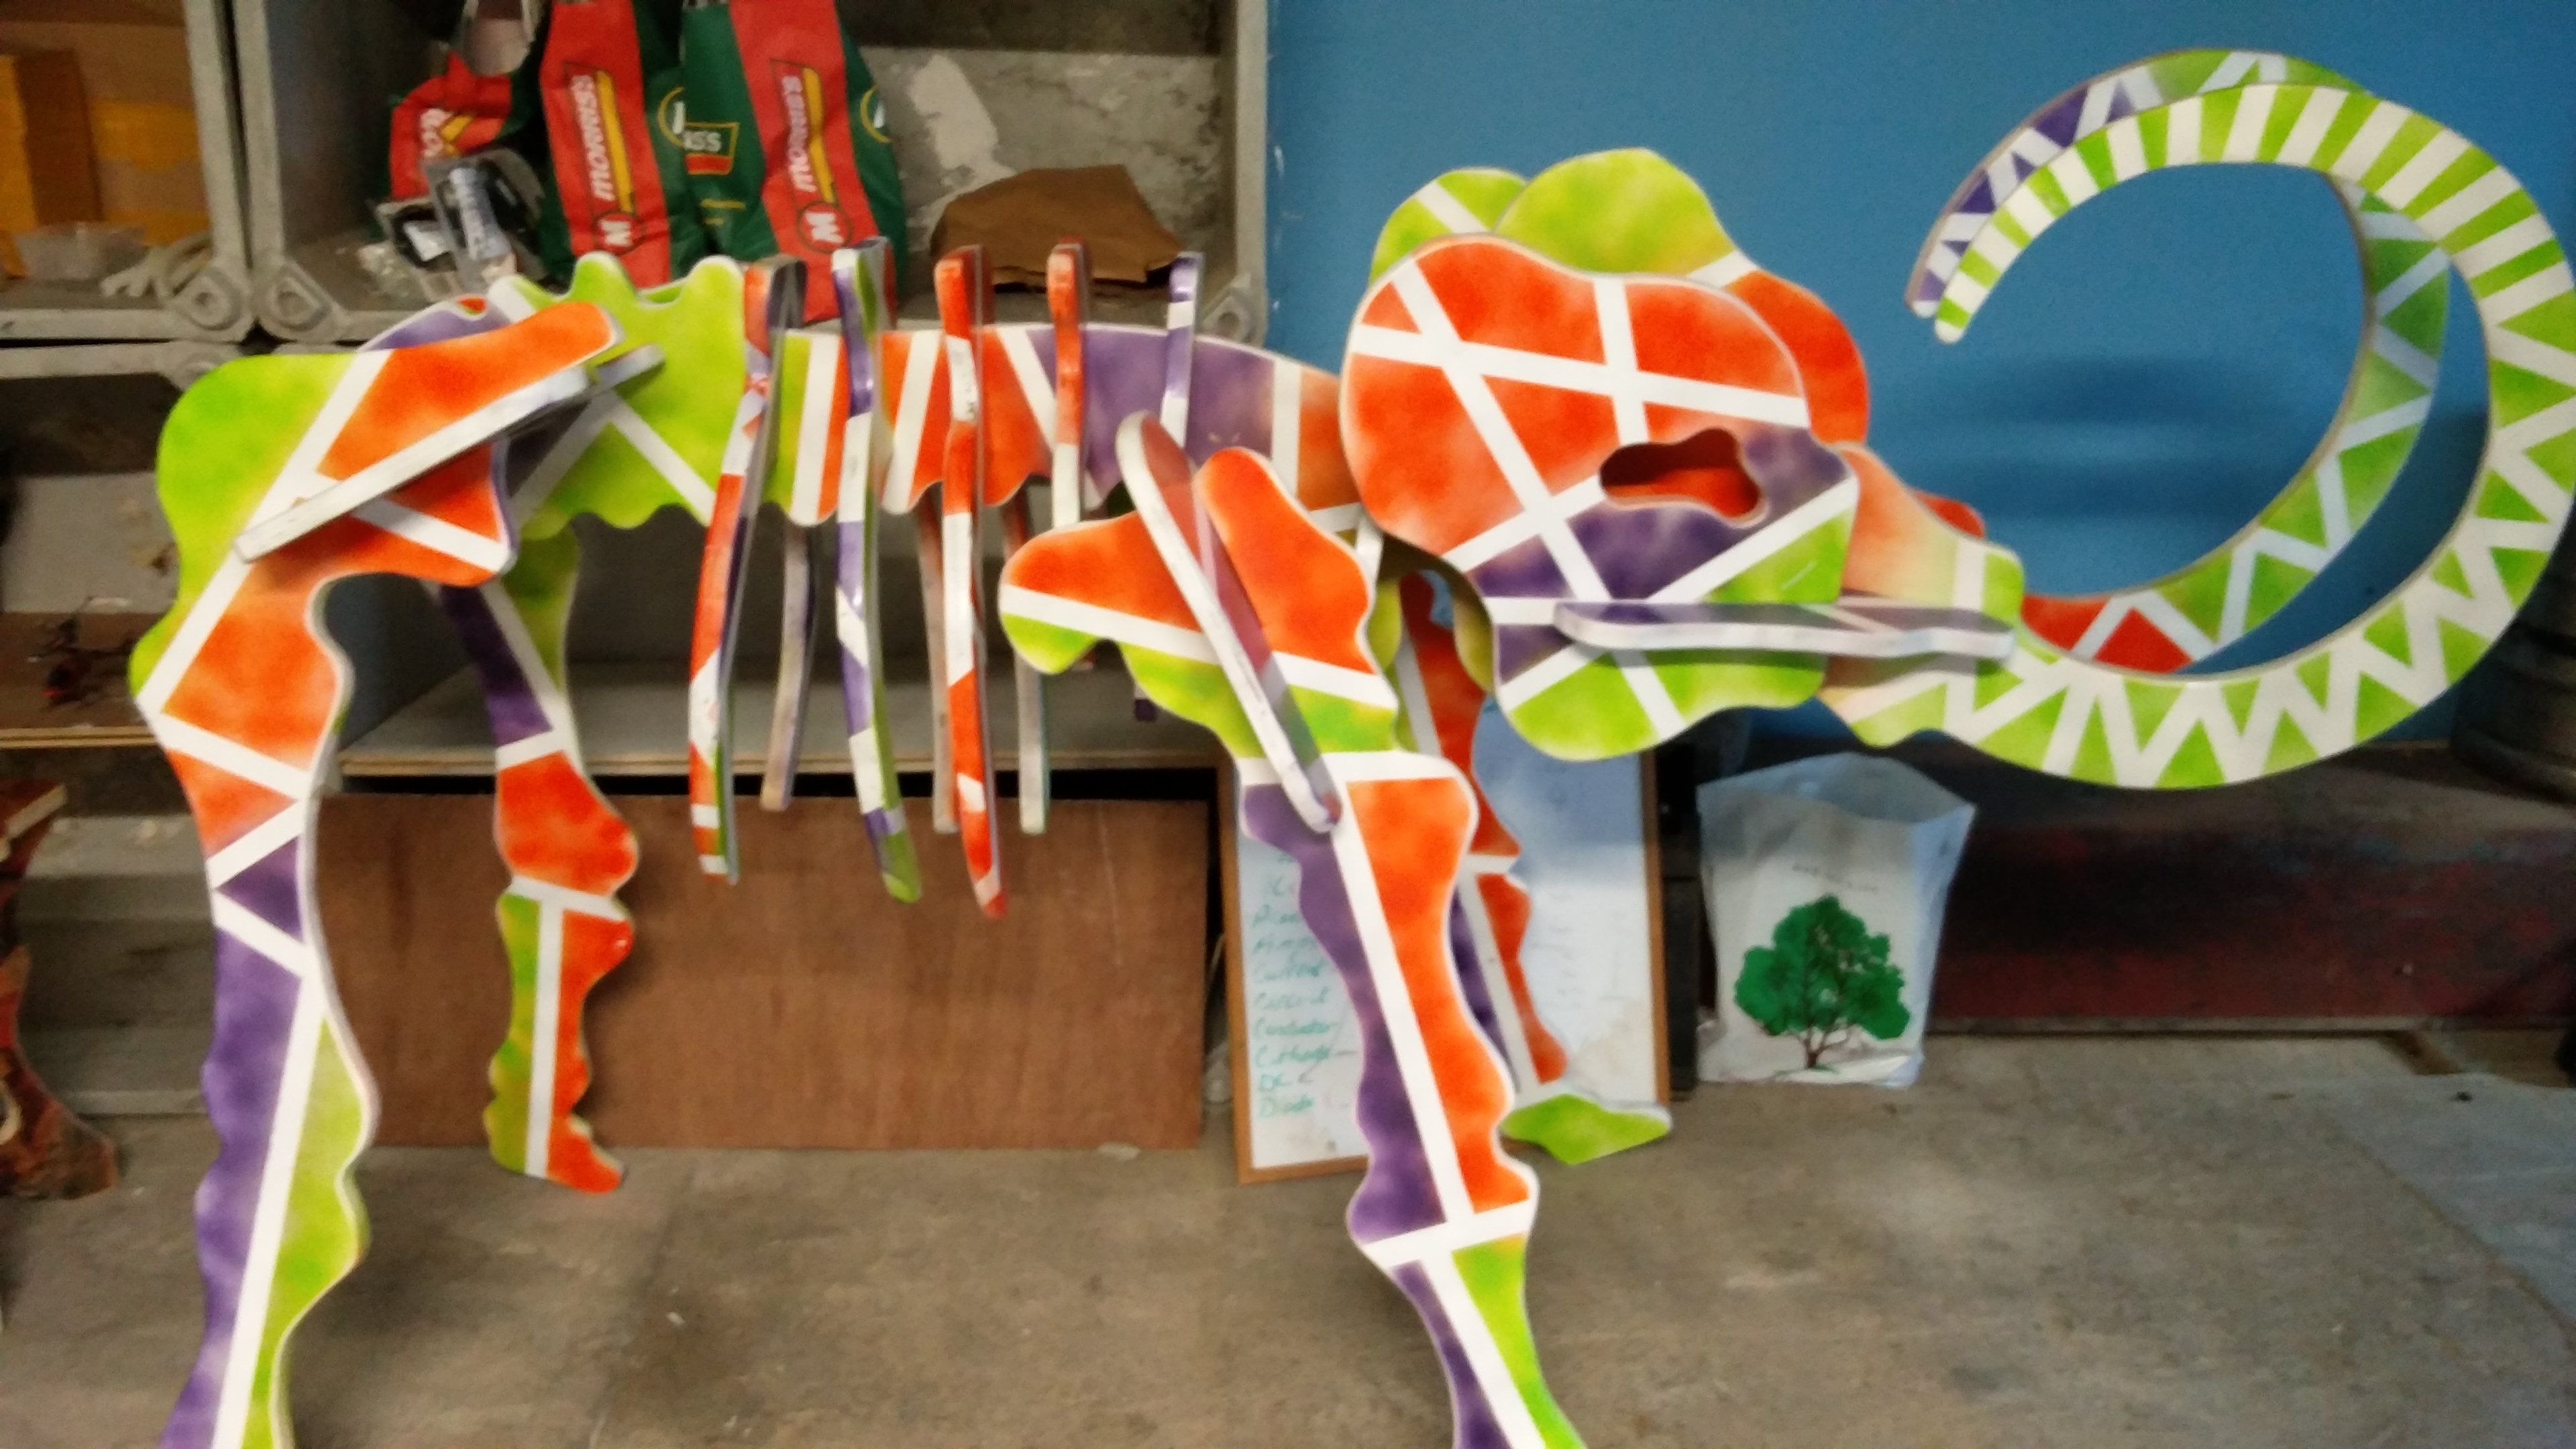
\includegraphics[width = 1.3in]{images/jig_6}} 
		\end{tabular}
		\caption{Jigsaw Dinosaurs 2016/2017}
	\end{figure}
\end{frame}


\section{Video Test}
\begin{frame}{Video Test}
	This is a YouTube video (needs an Internet connection to view):
	
	\href{http://www.youtube.com/v/g8Ejj0T0yG4?rel=0}{X}
\end{frame}


\end{document}
\endinput
%%
%% End of file `example_DarkConsole.tex'.
